\documentclass{./these-seb}


\usepackage[utf8]{inputenc}
\usepackage[T1]{fontenc}
\usepackage{babel}

\usepackage{textcomp}
\usepackage{pifont}
% Les polices possibles (pour tout le document)
%\usepackage[bitstream-charter]{mathdesign}

%Font ps pour le pdf
\usepackage{pslatex}
%Hyperliens pour le pdf
\usepackage[pdfauthor   = {Sébastien\ Le\ Roux},
    pdftitle = {From\ the\ source\ code\ to\ free\ software\ distribution:\ review\ and\ tips},
    pdfsubject = {From\ the\ source\ code\ to\ software\ distribution},
    pdfkeywords = {Linux\ GNU\ Make\ RPM\ DEB\ Git\ Github},
    pdfcreator = {Latex+DviPDF},
    pdfproducer = {LaTeX+DviPDF},
    pdfstartview=FitV   % Ouverture avec ajustement de l'image
    dvips=true,         % Use hyperref with dvips
    colorlinks=true,    % Lien hypertext en couleur
    plainpages=false,   %
    pagebackref=true,   % Permet d'ajouter des liens retour dans la biblio ...
    backref=page,       % .. ces liens pointent vers les 'pages' des citations
    hyperindex=true,    % Ajoute des liens dans l'index
    linktocpage=true,   % Lien sur les numéros de page et non le text 
    breaklinks=true,    % Permet le retour à la ligne dans les liens trop longs
    urlcolor= blue,     % Couleur des liens externes
%    linkcolor= black,   % Couleur des liens internes
    bookmarks=true,     % Création des signets pour Acrobat
    bookmarksopen=false % Toute l'arborescence est dépliée à l'ouverture
]{hyperref}
%\usepackage[pageref]{backref}

%Insertion d'images
\usepackage{graphicx}
\DeclareGraphicsExtensions{.eps}

%Dessins latex
% Brouillon ? = afficher les images "false" ou seulement les cadres "true"
% effet sur tout le document
\newcommand{\ddst}{false}
%\usepackage{picins}

\usepackage[x11names]{xcolor}

% Mode verbatim avancé
\usepackage{alltt}

% Système de liste/énumération
\usepackage{pifont}
\usepackage{enumerate}
%\usepackage{enumitem}

% Ecriture des mathématiques
\usepackage{amsmath}
\usepackage{amssymb}
\usepackage{amscd}
\usepackage{theorem}

% tableaux
\usepackage{hhline}
%\usepackage{array}
\usepackage{multirow}
\usepackage{tabls}
%\usepackage{bbding}

%% Mise en page
%\voffset         0.0cm
%\hoffset         0.0cm
%\textheight     23.0cm
%\textwidth      16.0cm
%\topmargin      -0.5cm
%\oddsidemargin   0.0cm
%\evensidemargin  0.0cm

% pages en landscape dans document portrait
\usepackage{lscape}

% Aspect de pages
\usepackage{setspace}
%\onehalfspacing
%\doublespacing
%\setstretch{3}

%\usepackage{fancyhdr,fancybox}
%\fancyhead{}
%\fancyhead[RO]{\scriptsize{\slshape\rightmark}}
%\fancyhead[LO]{\scriptsize{\thepage}}
%\fancyhead[RE]{\scriptsize{\thepage}}
%\fancyhead[LE]{\scriptsize{\slshape\leftmark}}
%\pagestyle{fancy}

% Numérotation pour les sous-sous-sections
\setcounter{secnumdepth}{3}
% Table des matières/figures/tables par chapitre
%\usepackage{minitoc}
% Pour placer des notes de bas de pages dans les titres
%\usepackage[stable]{footmisc}

%Définitions de théorèmes
\theoremstyle{plain}
\theoremheaderfont{\scshape}
\theorembodyfont{\normalfont\itshape}
\newtheorem{HK}{Théorème}

% notsotiny font size
\makeatletter
\newcommand\notsotiny{\@setfontsize\notsotiny{6.5}{7.6878}}
\newcommand\notsoscript{\@setfontsize\notsotiny{7}{8.339}}
\newcommand\notsofoot{\@setfontsize\notsofoot{9.5}{11.6}}
\makeatother

% Créer un environnement résumé
\def\abstract{
   \begin{center}
   \begin{minipage}{12cm}
   \begin{center}{\bf Résumé}\end{center}\par\small}
\def\endabstract{\par\end{minipage}\end{center}\vspace{1cm}}

% Bilblio:
% Bilblio:
\newcommand{\aap}{Astron. \& Astrophys.}
\newcommand{\aasup}{Astron. \& Astrophys. Suppl. Ser.}
\newcommand{\aj}{Astron. J.}
\newcommand{\aph}{Acta Phys.}
\newcommand{\act}{Acta Cryst.}
\newcommand{\actc}{Acta Cryst.}
\newcommand{\acta}{Acta Cryst. A}
\newcommand{\actb}{Acta Cryst. B}
\newcommand{\advp}{Adv. Phys.}
\newcommand{\ajp}{Amer. J. Phys.}
\newcommand{\ajm}{Amer. J. Math.}
\newcommand{\amsci}{Amer. Sci.}
\newcommand{\anofd}{Ann. Fluid Dyn.}
\newcommand{\am}{Ann. Math.}
\newcommand{\ap}{Ann. Phys. (NY)}
\newcommand{\adp}{Ann. Phys. (Leipzig)}
\newcommand{\ao}{Appl. Opt.}
\newcommand{\apl}{Appl. Phys. Lett.}
\newcommand{\app}{Astroparticle Phys.}
\newcommand{\apj}{Astrophys. J.}
\newcommand{\apjsup}{Astrophys. J. Suppl.}
\newcommand{\apss}{Astrophys. Space Sci.}
\newcommand{\araa}{Ann. Rev. Astron. Astrophys.}
\newcommand{\baas}{Bull. Amer. Astron. Soc.}
\newcommand{\baps}{Bull. Amer. Phys. Soc.}
\newcommand{\cmp}{Comm. Math. Phys.}
\newcommand{\cpam}{Commun. Pure Appl. Math.}
\newcommand{\cppcf}{Comm. Plasma Phys. \& Controlled Fusion}
\newcommand{\cpc}{Comp. Phys. Comm.}
\newcommand{\cms}{Comp. Mat. Sci.}
\newcommand{\cqg}{Class. Quant. Grav.}
\newcommand{\cra}{C. R. Acad. Sci. A}
\newcommand{\crv}{Chem. Rev.}
\newcommand{\cp}{Chem. Phys.}
\newcommand{\cma}{Chem. Mater.}
\newcommand{\epl}{Eur. Phys. Lett.}
\newcommand{\ejm}{Eur. J. Mineral.}
\newcommand{\fed}{Fusion Eng. \& Design}
\newcommand{\ft}{Fusion Tech.}
\newcommand{\grg}{Gen. Relativ. Gravit.}
\newcommand{\ieeens}{IEEE Trans. Nucl. Sci.}
\newcommand{\ieeeps}{IEEE Trans. Plasma Sci.}
\newcommand{\ijimw}{Interntl. J. Infrared \& Millimeter Waves}
\newcommand{\ip}{Infrared Phys.}
\newcommand{\irp}{Infrared Phys.}
\newcommand{\jap}{J. Appl. Phys.}
\newcommand{\jac}{J. Appl. Cryst.}
\newcommand{\jacs}{J. Am. Chem. Soc.}
\newcommand{\jamcs}{J. Am. Ceram. Soc.}
\newcommand{\jasa}{J. Acoust. Soc. America}
\newcommand{\jcp}{J. Chem. Phys.}
\newcommand{\jcop}{J. Comp. Phys.}
\newcommand{\jetp}{Sov. Phys.--JETP}
\newcommand{\jetpl}{JETP Lett.}
\newcommand{\jfe}{J. Fusion Energy}
\newcommand{\jfm}{J. Fluid Mech.}
\newcommand{\jmp}{J. Math. Phys.}
\newcommand{\jne}{J. Nucl. Energy}
\newcommand{\jnec}{J. Nucl. Energy, C: Plasma Phys., Accelerators, Thermonucl. Res.}
\newcommand{\jncs}{J. Non-Cryst. Solids.}
\newcommand{\jnm}{J. Nucl. Mat.}
\newcommand{\joam}{J. Optoelect. Adv. Mat.}
\newcommand{\jpcssp}{J. Phys. C: Solid State Phys.}
\newcommand{\jpc}{J. Phys. Chem.}
\newcommand{\jpcs}{J. Phys. Chem. Sol.}
\newcommand{\jpcm}{J. Phys.: Cond. Mat.}
\newcommand{\jpp}{J. Plasma Phys.}
\newcommand{\jpsj}{J. Phys. Soc. Japan}
\newcommand{\jqc}{J. Quant. Chem.}
\newcommand{\jssc}{J. Sol. Stat. Chem.}
\newcommand{\jsi}{J. Sci. Instrum.}
\newcommand{\jvst}{J. Vac. Sci. \& Tech.}
\newcommand{\mcp}{Mat. Chem. Phys.}
\newcommand{\molp}{Mol. Phys.}
\newcommand{\nat}{Nature}
\newcommand{\nature}{Nature}
\newcommand{\nedf}{Nucl. Eng. \& Design/Fusion}
\newcommand{\nf}{Nucl. Fusion}
\newcommand{\nim}{Nucl. Inst. \& Meth.}
\newcommand{\nimpr}{Nucl. Inst. \& Meth. in Phys. Res.}
\newcommand{\np}{Nucl. Phys.}
\newcommand{\npb}{Nucl. Phys. B}
\newcommand{\ntf}{Nucl. Tech./Fusion}
\newcommand{\npbpc}{Nucl. Phys. B (Proc. Suppl.)}
\newcommand{\inc}{Nuovo Cimento}
\newcommand{\nc}{Nuovo Cimento}
\newcommand{\pcg}{Phys. Chem. Glasses}
\newcommand{\pf}{Phys. Fluids}
\newcommand{\pfa}{Phys. Fluids A: Fluid Dyn.}
\newcommand{\pfb}{Phys. Fluids B: Plasma Phys.}
\newcommand{\pl}{Phys. Lett.}
\newcommand{\pla}{Phys. Lett. A}
\newcommand{\plb}{Phys. Lett. B}
\newcommand{\prep}{Phys. Rep.}
\newcommand{\pnas}{Proc. Nat. Acad. Sci. USA}
\newcommand{\pp}{Phys. Plasmas}
\newcommand{\ppcf}{Plasma Phys. \& Controlled Fusion}
\newcommand{\phitrsl}{Philos. Trans. Roy. Soc. London}
\newcommand{\plmb}{Phil. Mag. B} 
\newcommand{\pml}{Phil. Mag. Lett.}
\newcommand{\pmm}{Phil. Mag.}
\newcommand{\prl}{Phys. Rev. Lett.}
\newcommand{\pr}{Phys. Rev.}
\newcommand{\physrev}{Phys. Rev.}
\newcommand{\pra}{Phys. Rev. A}
\newcommand{\prb}{Phys. Rev. B}
\newcommand{\prc}{Phys. Rev. C}
\newcommand{\prd}{Phys. Rev. D}
\newcommand{\pre}{Phys. Rev. E}
\newcommand{\ps}{Phys. Scripta}
\newcommand{\pstb}{Phys. Stat. Sol. b}
\newcommand{\procrsl}{Proc. Roy. Soc. London}
\newcommand{\rmp}{Rev. Mod. Phys.}
\newcommand{\rsi}{Rev. Sci. Inst.}
\newcommand{\rpp}{Rep. Prog. Phys.}
\newcommand{\science}{Science}
\newcommand{\sciam}{Sci. Am.}
\newcommand{\susc}{Surf. Sci}
\newcommand{\sam}{Stud. Appl. Math.}
\newcommand{\sjpp}{Sov. J. Plasma Phys.}
\newcommand{\spd}{Sov. Phys.--Doklady}
\newcommand{\sptp}{Sov. Phys.--Tech. Phys.}
\newcommand{\spu}{Sov. Phys.--Uspeki}
\newcommand{\skt}{Sky and Telesc.}
\newcommand{\ssi}{Solid State Ionics}
\newcommand{\ssc}{Solid State Com.}
\newcommand{\ssnmr}{Solid State Nuc. Mag. Res.}
\newcommand{\zfp}{Zs. f. Phys.}
\newcommand{\zk}{Z. Kristallogr.}


%\usepackage{chapterbib}

\usepackage[square,comma,sort&compress]{natbib}
\usepackage{hypernat}

% Algo XML
\usepackage{listings}

% Texte souligné
\usepackage[normalem]{ulem}

% Mise en forme des légendes

\usepackage[hang]{caption}
%\renewcommand{\captionfont}{\it}
%\renewcommand{\captionlabelfont}{\bf}
%\renewcommand{\captionlabeldelim}{$\quad$}
\usepackage{subcaption}

\newcommand{\atomes}{{\em{\bf{atomes}}}}
\newcommand{\github}{\href{https://github.com}{GitHub}}
\newcommand{\gitlab}{\href{https://gitlab.com}{GitLab}}
\newcommand{\salsa}{\href{https://salsa.debian.org}{Salsa}}
\newcommand{\email}{your.email@host.eu}
\newcommand{\metamail}{your.email\_AT\_host.eu}
\newcommand{\gitauth}{https://github.com/Author}
\newcommand{\gitprog}{\gitauth/Program}
\newcommand{\tabul}{\hspace{0.5cm}}
%\usepackage[format=plain,labelfont=bf,up,textfont=it,up]{caption}
\newcommand{\red}[1]{\textcolor{red}{#1}}
\newcommand{\pink}[1]{\textcolor{pink}{#1}}
\newcommand{\green}[1]{\textcolor{green}{#1}}
\newcommand{\cyan}[1]{\textcolor{cyan}{#1}}
\definecolor{cadmium}{rgb}{0.05,0.5,0.06}
\newcommand{\dgreen}[1]{\textcolor{cadmium}{#1}}
\newcommand{\blue}[1]{\textcolor{blue}{#1}}
\newcommand{\brown}[1]{\textcolor{brown}{#1}}
\newcommand{\dblue}[1]{\textcolor{DodgerBlue4}{#1}}
\newcommand{\aqua}[1]{\textcolor{SpringGreen3}{#1}}
\newcommand{\magenta}[1]{\textcolor{magenta}{#1}}
\newcommand{\violet}[1]{\textcolor{violet}{#1}}
\definecolor{lg}{rgb}{0.95,0.95,0.95}
\newcommand{\rtt}[1]{{\bf{\texttt{\red{#1}}}}}
\newcommand{\gtt}[1]{{\bf{\texttt{\green{#1}}}}}
\newcommand{\dgtt}[1]{{\bf{\texttt{\dgreen{#1}}}}}
\newcommand{\btt}[1]{{\bf{\texttt{\blue{#1}}}}}
\newcommand{\dbtt}[1]{{\bf{\texttt{\dblue{#1}}}}}
\newcommand{\abtt}[1]{{\bf{\texttt{\aqua{#1}}}}}
\newcommand{\dctt}[1]{{\bf{\texttt{\cyan{#1}}}}}
\newcommand{\bbtt}[1]{{\bf{\texttt{\brown{#1}}}}}
\newcommand{\rgtt}[1]{\rtt{/}{\gtt{#1}}}
\newcommand{\rbtt}[1]{\rtt{/}{\btt{#1}}}
\newcommand{\bftt}[1]{{\bf{\texttt{#1}}}}

\usepackage{placeins}
\usepackage{keystroke}

% Créer un environnement codage bash
\newsavebox{\cobox}
\def\script{
  \noindent \\[0.25cm] \\
  \begin{lrbox}
  \cobox
  \begin{minipage}[l]{16cm}
  \begin{alltt}}
\def\endscript{
  \end{alltt}
  \end{minipage}
  \end{lrbox}
  \colorbox{lg}{\usebox{\cobox}}
  \vspace{0.25cm}\par\noindent}

% Idem mais avec puces (itemize) -1.0334 cm / puces
\newsavebox{\coboxi}
\def\scripti{
  \noindent \\[0.25cm] \\
  \begin{lrbox}
  \coboxi
  \begin{minipage}[l]{14.966cm}
  \begin{alltt}}
\def\endscripti{
  \end{alltt}
  \end{minipage}
  \end{lrbox}
  \colorbox{lg}{\usebox{\coboxi}}
  \vspace{0.25cm}\par\noindent}

\newsavebox{\coboxii}
\def\scriptii{
  \noindent \\[0.25cm] \\
  \begin{lrbox}
  \coboxii
  \begin{minipage}[l]{13.9332cm}
  \begin{alltt}}
\def\endscriptii{
  \end{alltt}
  \end{minipage}
  \end{lrbox}
  \colorbox{lg}{\usebox{\coboxii}}
  \vspace{0.25cm}\par\noindent}

\newsavebox{\coboxiii}
\def\scriptiii{
  \noindent \\[0.25cm] \\
  \begin{lrbox}
  \coboxiii
  \begin{minipage}[l]{12.9004cm}
  \begin{alltt}}
\def\endscriptiii{
  \end{alltt}
  \end{minipage}
  \end{lrbox}
  \colorbox{lg}{\usebox{\coboxiii}}
  \vspace{0.25cm}\par\noindent}

\newcommand{\fscript}[1]{{\footnotesize{\begin{script}#1\end{script}}}}
\newcommand{\sscript}[1]{{\scriptsize{\begin{script}#1\end{script}}}}

%Coloration synthaxique
\newcommand{\bash}{\textcolor{blue}{\#!/bin/bash}}
\newcommand{\bif}{\textcolor{brown}{{\bf{\texttt{if [}}}}}
\newcommand{\then}{\textcolor{brown}{{\bf{\texttt{]; then}}}}}
\newcommand{\bli}{\textcolor{brown}{{\bf{\texttt{elif [}}}}}
\newcommand{\bel}{\textcolor{brown}{{\bf{\texttt{else}}}}}
\newcommand{\bfi}{\textcolor{brown}{{\bf{\texttt{fi}}}}}
\newcommand{\blet}{\textcolor{brown}{{\bf{\texttt{let}}}}}
\newcommand{\bfor}{\textcolor{brown}{{\bf{\texttt{for}}}}}
\newcommand{\while}{\textcolor{brown}{{\bf{\texttt{while [}}}}}
\newcommand{\until}{\textcolor{brown}{{\bf{\texttt{until [}}}}}
\newcommand{\bin}{\textcolor{brown}{{\bf{\texttt{in}}}}}
\newcommand{\bdo}{\textcolor{brown}{{\bf{\texttt{do}}}}}
\newcommand{\done}{\textcolor{brown}{{\bf{\texttt{done}}}}}
\newcommand{\comm}[1]{\textcolor{blue}{\# #1}}
\newcommand{\var}[1]{\textcolor{cyan}{#1}}
\newcommand{\dvar}[1]{\textcolor{violet}{\$#1}}
\newcommand{\vard}[1]{\$#1}
\newcommand{\varc}[1]{\dgtt{\$\{#1\}}}
\newcommand{\echo}{\textcolor{brown}{{\bf{\texttt{echo}}}}}
\newcommand{\bcp}{\textcolor{brown}{{\bf{\texttt{cp}}}}}
\newcommand{\cd}{\textcolor{brown}{{\bf{\texttt{cd}}}}}
\newcommand{\mv}{\textcolor{brown}{{\bf{\texttt{mv}}}}}
\newcommand{\brm}{\textcolor{brown}{{\bf{\texttt{rm}}}}}
\newcommand{\mkdir}{\textcolor{brown}{{\bf{\texttt{mkdir}}}}}
\newcommand{\mkdirp}{\textcolor{brown}{{\bf{\texttt{mkdir -p}}}}}
\newcommand{\bnum}[1]{\textcolor{red}{\texttt{#1}}}
\newcommand{\say}[1]{\textcolor{brown}{"}\textcolor{magenta}{#1}\textcolor{brown}{"}}
\newcommand{\beq}{\textcolor{brown}{{\bf{\texttt{-eq}}}}}
\newcommand{\bne}{\textcolor{brown}{{\bf{\texttt{!=}}}}}
\newcommand{\bap}{\textcolor{brown}{\texttt{"}}}
\newcommand{\pipe}{\textcolor{brown}{{\bf{\texttt{|}}}}}
\newcommand{\svar}[1]{\textcolor{blue}{\texttt{`#1`}}}
\newcommand{\reg}[1]{\bbtt{\textquotesingle}\magenta{#1}\bbtt{\textquotesingle}}
\newcommand{\bad}[1]{\textcolor{brown}{{\bf{\texttt{#1}}}}}
\newcommand{\lint}{\bftt{lintian}}
\newcommand{\piup}{\rtt{sudo} \bftt{piuparts}}
\newcommand{\func}[1]{\textcolor{cyan}{{\bf{\texttt{function #1 \{ }}}}}
\newcommand{\efunc}{\textcolor{cyan}{{\bf{\texttt{\}}}}}}
\newcommand{\yml}[1]{\cyan{\texttt{#1}}\bbtt{:}}

%markdown:
\newcommand{\mdcom}[1]{\textcolor{cyan}{\texttt{<!-{-} #1 -{-}>}}}

% prompt
\newcommand{\uprompt}[1]{\dgtt{user@localhost}:\btt{#1}\$}
\newcommand{\fprompt}[1]{user@localhost #1]\$}
\newcommand{\lsr}{\bftt{ls} \rtt{-R}}

% configure
\newcommand{\bmpt}[2]{\begin{minipage}{3cm}#1\end{minipage} & $\Longrightarrow$ & 
	\begin{minipage}{12cm}#2\end{minipage} \\ \\ \\}
\newcommand{\dnl}[1]{\textcolor{blue}{dnl #1}}
\newcommand{\cpink}[1]{\textcolor{pink}{\texttt{#1}}}
\newcommand{\confa}[1]{\textcolor{cyan}{{\bf{\texttt{#1}}}}}
\newcommand{\confb}[2]{\textcolor{cyan}{{\bf{\texttt{#1(}}}}#2\textcolor{cyan}{{\bf{\texttt{)}}}}}
\newcommand{\cstr}[1]{\dgtt{[}#1\dgtt{]}}
\newcommand{\cacf}[5]{\confb{#1}{\cstr{\rtt{#2}}, \cstr{#3}, \cstr{#4}, \cstr{#5}}}
\newcommand{\cact}[4]{\confb{#1}{\cstr{\rtt{#2}}, \cstr{#3}, \cstr{#4}}}
\newcommand{\cacb}[3]{\confb{#1}{\cstr{\rtt{#2}}, \cstr{#3}}}

% Command
\newcommand{\cmd}[4]{
\begin{itemize}
\item
\begin{tabular*}{0.95\textwidth}{l@{\extracolsep{\fill}}r}
\textcolor{blue}{\bf{\texttt{#1}}} & {\it{"#2"}}
\end{tabular*} \\
\hspace{1cm} - usage:\quad {\bf{\texttt{#1 #3}}} \\
\hspace{1cm} - ex:   \quad \texttt{ user@localhost ]\$ #1 #4}
\end{itemize}
}
% Command with options
\newcommand{\cmdo}[5]{
\begin{itemize}
\item
\begin{tabular*}{0.95\textwidth}{l@{\extracolsep{\fill}}r}
\textcolor{blue}{\bf{\texttt{#1}}} & {\it{"#2"}} 
\end{tabular*} \\
\hspace{1cm} - usage:\quad {\bf{\texttt{#1 #3}}} \\
\hspace{1cm} - ex:   \quad \texttt{ user@localhost ]\$ #1 #4} \\
\hspace{1cm} - options: #5
\end{itemize}
}
% Command with redirection
\newcommand{\cmdr}[4]{
\begin{itemize}
\item
\begin{tabular*}{0.95\textwidth}{l@{\extracolsep{\fill}}r}
\textcolor{blue}{\bf{\texttt{#1}}} & {\it{"#2"}}
\end{tabular*} \\
\hspace{1cm} - usage:\quad {\bf{\texttt{#3}}} \\
\hspace{1cm} - ex:   \quad \texttt{ user@localhost ]\$ #4}
\end{itemize}
}

% Custom environemnts for the tables 'tableh' and figures 'figureh'
% to deal both with font size and the centering, so that you do not need to use 
% a \begin{center} and \end{center} each time
% You can adapt it to your liking by changing the font size command \scriptsize
\def\tableh{
  \begin{table}[h!]\centering}
  \def\endtableh{\par\end{table}}

\def\figureh{
  \begin{figure}[h!]\centering}
\def\endfigureh{\par\end{figure}}

\def\tablep{
  \begin{table}[p!]\centering}
  \def\endtablep{\par\end{table}}

\def\figurep{
  \begin{figure}[p!]\centering}
\def\endfigurep{\par\end{figure}}


\includeonly{greats, build/build, git/git, hosting/hosting, packaging/packaging, appendix/appendix}
%\includeonly{greats, build/build, appendix/appendix}
%\includeonly{git/git}
%\includeonly{hosting/hosting}
%\includeonly{packaging/packaging}

\begin{document}

% Préparation pour mini-table des matières, des figures et des tables si besoin
%\dominitoc
%\dominilof
%\dominilot

%
\newcommand{\ubuntu}{Ubuntu }
\renewcommand{\figurename}{Figure}
\renewcommand{\tablename}{Table}

\titleEN{From source code\\ to packaging:\\ open source software\\ distribution review and tips\\}

\author{Sébastien {\sc{Le Roux}}\quad\href{mailo:sebastien.leroux@ipcms.unistra.fr}{sebastien.leroux@ipcms.unistra.fr}}
\universite{Institut de Physique et de Chimie des Mat\'eriaux de Strasbourg, \\
D\'epartement des Mat\'eriaux Organiques, \\
23 rue du Loess, BP43, \\ F-67034 Strasbourg Cedex 2, France\\[0.25cm]{\textrm{\today}}}

\beforepreface
\setcounter{page}{1}            % Je recommence la numerotation a un pour pas
                                % decaler l'alternance droite/gauche et que
                                % les pages impaires soient bien a droite.

\def\greats#1{\gdef\greatings@text{#1}}
\greats{\chapter*{Acknowledgments}

You are about to read a document I decided to write after packaging my own software \href{https://atomes.ipcms.fr}{atomes} for the \href{https://fedoraproject.org}{Fedora} and \href{https://www.debian.org}{Debian} Linux distributions. 
I wanted to put together the results of theses experiences so that it could help others to take advantage of the fantastic opportunities of the open source communities. \\[0.25cm]
But the fact is that I am neither a specialist of building systems, git, GitHub, GitLab, RPM or even Debian packaging. 
I merely have now a broad perspective of the whole system. \\[0.25cm]
I had help, to say the least, along the way. \\[0.25cm]
Help when I pushed open the doors of the Fedora and the Debian communities where I got lucky to find people who supported \href{https://atomes.ipcms.fr}{atomes}, 
and took the time to teach me to make it happen ... not only that but they also accepted to proof read this document afterwards, crazy ... thank you so, so, very much: 
\begin{itemize}
\item My \href{https://fedoraproject.org}{Fedora} mentor: {\bf{Alexander Ploumistos}}
\item My \href{https://www.debian.org}{Debian} mentor: {\bf{Pierre Gruet}}
\end{itemize}
I also have to thank Sylvain Thery, a colleague and Git specialist, who kindly destroyed the first version of the Git chapter of this manual. 

}

\greatings@text\vfill
\cleardoublepage

%\setcounter{tocdepth}{4}

% Mise en forme TOC/TOF/LOT
{\small \tableofcontents}
\addcontentsline{toc}{chapter}{Contents}
%{\it \footnotesize \listoffigures}
%\addcontentsline{toc}{chapter}{List of figures}
%\chaptermark{List of figures}
%{\it \footnotesize \listoftables}
%\addcontentsline{toc}{chapter}{List of tables}
%\chaptermark{List of tables}

\afterpreface

\vfill                          % Je remplis avec du rien (\vfill}
\pagebreak                      % Je change de page.
%{\small \printindex}

\chapter*{Introduction}
\addcontentsline{toc}{chapter}{Introduction}
\chaptermark{Introduction}
\markboth{Introduction}{Introduction} 

\section*{Purpose}
\addcontentsline{toc}{section}{Purpose}

The purpose of this tutorial is to introduce the essential steps required to publish an open source software. 
It is both a personal review of the process and a collection of tips, intended to help the programmer navigates from its source code up to free software distribution. \\
It is not, and does not aim to be comprehensive, but to be a proper recollection of my own experiences, so that these could help others. 

\section*{Prerequisites}
\addcontentsline{toc}{section}{Prerequisites}


In the following I will consider that the reader is familiar with using the command line. \\
To learn more about the command line and Linux check out my \href{https://www.ipcms.fr/wp-content/uploads/2021/11/linux.pdf}{Linux tutorial}. \\
To learn more about scripting and advanced command line use check out my \href{https://www.ipcms.fr/wp-content/uploads/2021/05/bash.pdf}{Bash tutorial}. 

\section*{Target readers}
\addcontentsline{toc}{section}{Target readers}

Any one who want to publish an open source program, in particular if that person is interested in having its code distributed within the Linux open source community. 

\newpage

\section*{Software build}
\addcontentsline{toc}{section}{Software build}

Starting from the next chapter I will consider that you already have a piece of code written and ready to be used, even ready to be distributed. 
The programming language does not matter, I will simply focus on what comes next. \\[0.25cm]
The example I will use through out this tutorial is based on my \href{https://atomes.ipcms.fr}{Atomes} software, 
and will offer various illustrations for the build automation process, packaging and distribution of a code that requires: 
\begin{itemize}
\item To be built using:
\begin{itemize}
\item The \href{https://www.gnu.org/software/gcc/}{gcc} compiler (part of the sources are in C).
\item The \href{https://gcc.gnu.org/wiki/GFortran}{gfortran} compiler (part of the sources are if Fortran90).
\end{itemize}
\item To be linked with:
\begin{itemize}
\item The \href{https://www.gtk.org/}{GTK3} library.
\item The \href{http://xmlsoft.org/}{libxml2} library.
\item The \href{https://gitlab.freedesktop.org/mesa/glu}{MESA GLu} library.
\item The \href{https://github.com/anholt/libepoxy}{libepoxy} library.
\item The \href{https://ffmpeg.org}{FFMPEG} libraries (libavcodec, libavformat, libavutil, libswscale)
\end{itemize}
\end{itemize}
\vspace{0.25cm}
\noindent Our concern will be focused on the software building process, that is the process of converting source code file(s) into standalone software(s) 
that can be run on a computer (see \href{https://en.wikipedia.org/wiki/Software\_build}{software build process on Wikipedia}), and, 
the build automation process, that is the automating of the creation of a software build and the associated tasks (compiling, packaging, testing ...) (see \href{https://en.wikipedia.org/wiki/Build\_automation}{build automation on Wikipedia}).  

\chapter{Building system and automation}

In order to distribute your code it is almost mandatory to have a build system in mind, that is an automation tool that will help you to build your software using the sources, link it with used libraries, and even handle the installation process. \\
Historically build automation was handled using basic Makefile(s), but now more advanced tools are available, the most well known likely being:
\begin{itemize}
\item \href{https://en.wikipedia.org/wiki/Make\_(software)}{Make} 
\item \href{https://en.wikipedia.org/wiki/CMake}{CMake}
\item \href{https://en.wikipedia.org/wiki/Meson\_(software)}{Meson}
\end{itemize}
But there are many others. \\
In the following I will present examples using:
\begin{itemize}
\item The \href{https://www.gnu.org/software/make/}{GNU Make} implementation of the Make building system. 
The GNU Make is a standard distribution format, if your are familiar with open source software it is likely that your already stumbled upon a GNU tarball (or archive), 
either in Gzip of Bzip2 format:
\begin{itemize}
\item {\bftt{program.tar.gz}}, to be opened using: \begin{script}\fprompt{~} tar -zxf program.tar.gz\end{script}
\item {\bftt{program.tar.bz2}}, to be opened using: \begin{script}\fprompt{~} tar -jxf program.tar.bz2\end{script}
\end{itemize}
Very often the content of this archive is based on the GNU automation build system. 
In the following I will provide an example of the preparation of basic GNU tarball, that represents the first step in distributing your software to the open source community.
\item The \href{https://cmake.org/}{CMake} cross-platform open-source software for build automation, testing, packaging and installation of software by using a compiler-independent method. \\
\href{https://cmake.org/}{CMake} is not a build system itself, it generates another system's build files and can invoke native building environments such as Make. 
\item The modern \href{https://mesonbuild.com}{meson} build system written in Python. \\
Meson is desinged to provide simple, out-of-the-box support for modern software development tools and practises.
\end{itemize}

\section{The GNU Autotools}

The GNU Autotools, also known as the GNU Build System, is a suite of programming tools designed to assist in making source code packages portable (see \href{https://en.wikipedia.org/wiki/GNU\_Autotools}{GNU Autotools on Wikipedia}).  \\[0.25cm]
Autotools consists of the GNU utility programs: \href{https://www.gnu.org/software/autoconf/}{Autoconf}, 
\href{https://www.gnu.org/software/automake/}{Automake}, and \href{https://www.gnu.org/software/libtool}{Libtool}. \\
Other related tools are frequently used alongside it: 
\begin{itemize}
\item \href{https://www.gnu.org/software/make/}{GNU's make} program
\item \href{https://www.gnu.org/software/gettext/}{GNU gettext}
\item \href{https://en.wikipedia.org/wiki/Pkg-config}{pkg-config}
\item \href{https://www.gnu.org/software/gcc/}{GNU Compiler Collection}, also called GCC. 
\end{itemize}
Before going further into this guide, and if you want to try to build your own GNU tarball, you will have to install some of these tools: 
\begin{itemize}
\item For Windows and OSX please refer to the corresponding websites.
\item For Linux you can quite conveniently use the command line as follow:
\begin{itemize}
\item Red Hat based Linux (using the \bftt{dnf} command):
\begin{scriptii}
\fprompt{~} sudo \bftt{dnf} install autoconf automake libtool
\fprompt{~} sudo \bftt{dnf} install pkg-config gcc gcc-gfortran
\end{scriptii}
\item Debian based Linux (using the \bftt{apt} command):
\begin{scriptii}
\fprompt{~} sudo \bftt{apt} install autoconf automake libtool
\fprompt{~} sudo \bftt{apt} install pkg-config gcc gfortran
\end{scriptii}
\end{itemize}
\end{itemize}
To learn more about software installation on Linux check out my \href{https://www.ipcms.fr/wp-content/uploads/2021/11/linux.pdf}{Linux tutorial}. \\
To learn more about scripting and the usage of the command line check out my \href{https://www.ipcms.fr/wp-content/uploads/2021/05/bash.pdf}{Bash tutorial}.
\clearpage

\subsection{The GNU tarball or GNU archive}

A GNU tarball (archive) is a common way to distribute open source software built using the GNU Autotools, along with the sources of the program it should contain all the following files: \\[0.75cm]
\begin{tabular}{lcp{13cm}}
\bmpt{\rtt{configure.ac}}{A configuration file that defines the compilation options for the project, \\
and the rules to generate the \bftt{configure} script to create the tarball.}
\bmpt{\gtt{configure}}{A script generated using the \bftt{configure.ac} file. \\
It is used to configure the compilation and installation options \\
based on the operating system and development environment.}
\bmpt{\rtt{Makefile.am}}{A file that contains the build rules for the project. \\
It is used to generate the \bftt{Makefile.in} file.}
\bmpt{\bftt{Makefile.in}}{A file used by the \bftt{configure} script to generate the \bftt{Makefile}.}
\bmpt{\bftt{README(.md)}}{A file that contains important information about the project, \\ such as installation and usage instructions.}
\bmpt{\bftt{INSTALL(.md)}}{A file that contains installation instructions for the project.}
\bmpt{\bftt{AUTHORS(.md)}}{A file that contains information about the author(s) of the project.}
\bmpt{\bftt{COPYING(.md)}}{A file that contains the terms of the license \\ under which the project is distributed.}
\bmpt{\bftt{ChangeLog}}{A file that contains a list of changes made to the project \\ since the last release.}
\bmpt{\bftt{NEWS(.md)}}{A file that contains information about new features \\ or significant changes made to the project.}
\end{tabular}
%\begin{itemize}
%\item \bftt{configure}\\[0.25cm]
%A script generated using the \bftt{configure.ac} file. It is used to configure the compilation and installation options for the project based on the operating system and development environment.
%\item \rtt{Makefile.am}\\[0.25cm]
%A file that contains the build rules for the project. It is used to generate the file \bftt{Makefile.in} used by the \bftt{configure} script to generate the \bftt{Makefile}.
%\item \bftt{Makefile.in}\\[0.25cm] A file that used by the \bftt{configure} script to generate the \bftt{Makefile}.
%\item \bftt{README}\\[0.25cm]
%A file that contains important information about the project, such as installation and usage instructions.
%\item \bftt{INSTALL}\\[0.25cm] A file that contains installation instructions for the project.
%\item \bftt{AUTHORS}\\[0.25cm] A file that contains information about the author(s) of the project.
%\item \bftt{COPYING}\\[0.25cm] A file that contains the terms of the license under which the project is distributed.
%\item \bftt{ChangeLog}\\[0.25cm] A file that contains a list of changes made to the project since the last release.
%\item \bftt{NEWS}\\[0.25cm] A file that contains information about new features or significant changes made to the project.
%\end{itemize}
\clearpage
\noindent In order to prepare a GNU tarball it is mandatory to edit and prepare the following files:
\begin{itemize}
\item The \rtt{configure.ac} file.
\item The \rtt{Makefile.am} file(s) \\
There is usually one file in the upper directory of the archive. 
However if the sources are organized in the form of a directory tree you might want to provide multiple \bftt{Makefile.am} file(s), 
one at each significant level in the directory tree, this will help to simply the organization of the build process. 
\end{itemize}
At the build process of the GNU archive it is mandatory to have prepared all \bftt{Makefile.am} file(s) before being able to process the \bftt{configure.ac} file with \bftt{autoconf}. \\[0.25cm]
The next sections will illustrate the creation of these 2 files. 

\clearpage
\subsection{The file: \bftt{configure.ac}}

To start working on your GNU tarball you will need first to create a directory to work in:
\begin{script}
\fprompt{~} mkdir program
\fprompt{~} cd program
\end{script}
\\
\noindent Then use the \bftt{autoscan} command to generate à \bftt{configure.scan} file, 
and rename this file as \bftt{configure.ac} (you can also remove the empty \bftt{autoscan.log} file: 
\begin{script}
\fprompt{~/program} \bftt{autoscan}
\fprompt{~/program} rm -f autoscan.log
\fprompt{~/program} mv configure.scan \bftt{configure.ac}
\end{script}
\\
\noindent Then by editing the \bftt{configure.ac} file you will see that it follows the general structure:
{\footnotesize{
\begin{script}
\dnl{In a \bftt{configure.ac} file, commented line(s), could start by either:}
\dnl{\tabul- '\bftt{dnl}' and will not appear in the resulting \bftt{configure} script}
\dnl{\tabul- '\bftt{#}' and will appear in the resulting \bftt{configure} script}

\comm{Using the instructions AC\_INIT and AC\_INIT\_AUTOMAKE - see [Sec. \ref{cinit}].}
\confb{AC\_INIT}{\cstr{FULL-PACKAGE-NAME}, \cstr{VERSION}, \cstr{BUG-REPORT-ADDRESS}}
\confa{AM\_INIT\_AUTOMAKE}

\comm{Checks for program(s) - see [Sec. \ref{cprog}].}

\comm{Check for compiler(s) - see [Sec. \ref{ccomp}].}

\comm{Check for libraries - see [Sec. \ref{clibs}].}

\comm{Using the instruction AC\_CONFIG\_FILES and AC\_OUTPUT - see [Sec. \ref{cfinal}].}
\confa{AC\_CONFIG\_FILES}
\confa{AC\_OUTPUT}
\end{script}
}}
\\
\noindent In the following I will provide commented examples of the different parts of a standard \bftt{configure.ac} file, a complete file can be found in appendix [App.~\ref{configall}]. 
\clearpage

\subsubsection{Initialization}
\label{cinit}

The \bftt{configure.ac} always start with a mandatory \bftt{AC\_INIT} instruction. \\[0.25cm]
Everything before \bftt{AC\_INIT} is optional. \\[0.25cm]
A detailed example is provided thereafter to initialize your \bftt{configure.ac} file:
{\footnotesize{
\begin{script}
\dnl{Ensure to use a minimum version of Autoconf:}
\confb{AC\_PREREQ}{\red{2.59}}

\dnl{Defining local variables for major, minor and patch version(s) of the program:}
m4\_define(\bftt{major\_version}, \red{1})
m4\_define(\bftt{minor\_version}, \red{2})
m4\_define(\bftt{patch\_version}, \red{12})
\dnl{Defining local variable for the global version of the program:}
m4\_define(\bftt{version}, \bftt{major\_version}\rtt{.}\bftt{minor\_version}\rtt{.}\bftt{patch\_version})
\dnl{Defining local variable for the bug report email:}
m4\_define(\bftt{bug\_email}, \red{\email})
\dnl{Defining local variable for the name of the tarball:}
m4\_define(\bftt{tar\_name}, \red{program})
\dnl{Defining local variable for the project URL:}
m4\_define(\bftt{project\_url}, \red{https://www.program.com})

\dnl{AC\_INIT: performs initialization and verification.}
\dnl{This will define number of variables used afterwards:}
\dnl{\tabul AC\_PACKAGE\_NAME}
\dnl{\tabul AC\_PACKAGE\_VERSION}
\dnl{\tabul AC\_PACKAGE\_BUGREPORT}
\dnl{\tabul AC\_PACKAGE\_TARNAME}
\dnl{\tabul AC\_PACKAGE\_URL}
\confb{AC\_INIT}{\cstr{\bftt{prog}}, \cstr{\bftt{version}}, \cstr{\bftt{bug\_email}}, \cstr{\bftt{tar\_name}}, \cstr{\bftt{project\_url}}}

\dnl{AM\_INIT\_AUTOMAKE: initializes the Automake build system}
\dnl{It will set up the build environment, using all previously defined variables:}
\confa{AM\_INIT\_AUTOMAKE}

\dnl{Defining pre-processor variables for program version(s), major, minor and patch:}
\dnl{\tabul AC\_DEFINE([VAR\_NAME], [VALUE], [String])}
\dnl{Then replace all instances of VAR\_NAME in the output file(s) by VALUE}
\dnl{\tabul AC\_SUBST(VAR\_NAME, [VALUE])}
\confb{AC\_DEFINE}{MAJOR\_VERSION, \bftt{major\_version}, \cstr{Program major version}}
\confb{AC\_SUBST}{MAJOR\_VERSION, \bftt{major\_version}}
\confb{AC\_DEFINE}{MINOR\_VERSION, \bftt{minor\_version}, \cstr{Program minor version}}
\confb{AC\_SUBST}{MINOR\_VERSION, \bftt{minor\_version}}
\confb{AC\_DEFINE}{PATCH\_VERSION, \bftt{patch\_version}, \cstr{Program patch version}}
\confb{AC\_SUBST}{PATCH\_VERSION, \bftt{patch\_version}}
\end{script}
}}

\subsubsection{Checking for program(s)}
\label{cprog}

At some point you will need to check for the required tools and libraries. 
The easiest way to do this is by using the \bftt{AC\_CHECK\_*} macros provided by GNU autotools. \\[0.25cm]
The most convenient way to check for library/libraries is to use the command \bftt{pkg-config}, however you need
to make sure that this command is available on the target system, and therefore you need to check if the program 
\bftt{pkg-config} has been installed: 
{\footnotesize{
\begin{script}
\dnl{This will check that \bftt{program} is installed.}
\dnl{It will also set the \bftt{variable} to the path of the \bftt{program} executable.}
\dnl{\tabul AC\_CHECK\_PROG ([variable], [program], [text-if-found], [text-if-not-found])}
\confb{AC\_CHECK\_PROG}{[PKG\_CONFIG], [pkg-config], [yes], [no])}
\dnl{Checking for utilities need for Freedesktop Linux integration, see [Sec. \ref{rpmpost}]:}
\confb{AC\_CHECK\_PROG}{[UP\_MIME], [update-mime-database], [yes], [no]}
\confb{AC\_CHECK\_PROG}{[UP\_DESKTOP], [update-desktop-database], [yes], [no]}
\confb{AC\_CHECK\_PROG}{[UP\_APPSTREAM], [appstream-util], [yes], [no]}
\end{script}
}}
\vspace{-1cm}
\subsubsection{Checking for compiler(s)}
\label{ccomp}

The following examples illustrate how to check if: 
\begin{itemize}
\item User defined compilers flags are suitable to build the program:
\vspace{-0.25cm}
{\footnotesize{
\begin{scripti}
\dnl{Compiler(s) flags checking}
\dnl{For some reason the AX\_CHECK\_COMPILER\_FLAGS is broken}
\dnl{It is required to use this piece of code to define a proper test function:}
\confb{AC\_DEFUN}{[AX\_CHECK\_COMPILER\_FLAGS],
\tabul [AC\_PREREQ(\red{2.59}) \dnl{for \_AC\_LANG\_PREFIX}
\tabul AC\_MSG\_CHECKING([whether \_AC\_LANG compiler accepts \$1])
\tabul \confb{AS\_LITERAL\_IF}{[\$1],
\tabul\tabul [AC\_CACHE\_VAL(AS\_TR\_SH(ax\_cv\_[]\_AC\_LANG\_ABBREV[]\_flags\_\$1), [
\tabul\tabul\tabul ax\_save\_FLAGS=\$[]\_AC\_LANG\_PREFIX[]FLAGS
\tabul\tabul\tabul \_AC\_LANG\_PREFIX[]FLAGS="\$1"
\tabul\tabul\tabul C\_COMPILE\_IFELSE([AC\_LANG\_PROGRAM()],
\tabul\tabul\tabul AS\_TR\_SH(ax\_cv\_[]\_AC\_LANG\_ABBREV[]\_flags\_\$1)=yes,
\tabul\tabul\tabul AS\_TR\_SH(ax\_cv\_[]\_AC\_LANG\_ABBREV[]\_flags\_\$1)=no)
\tabul\tabul \_AC\_LANG\_PREFIX[]FLAGS=\$ax\_save\_FLAGS])],
\tabul\tabul [ax\_save\_FLAGS=\${[]\_AC\_LANG\_PREFIX[]FLAGS}
\tabul\tabul \_AC\_LANG\_PREFIX[]FLAGS="\$1"
\tabul\tabul AC\_COMPILE\_IFELSE([AC\_LANG\_PROGRAM()],
\tabul\tabul\tabul eval AS\_TR\_SH(ax\_cv\_[]\_AC\_LANG\_ABBREV[]\_flags\_\$1)=yes,
\tabul\tabul\tabul eval AS\_TR\_SH(ax\_cv\_[]\_AC\_LANG\_ABBREV[]\_flags\_\$1)=no)
\tabul\tabul \_AC\_LANG\_PREFIX[]FLAGS=\$ax\_save\_FLAGS]}
\tabul eval ax\_check\_compiler\_flags=\${AS\_TR\_SH}(ax\_cv\_[]\_AC\_LANG\_ABBREV[]\_flags\_\$1)
\tabul AC\_MSG\_RESULT(\$ax\_check\_compiler\_flags)
\tabul if test "x\$ax\_check\_compiler\_flags" = xyes; then
\tabul\tabul m4\_default([\$2], :)
\tabul else
\tabul\tabul m4\_default([\$3], :)
\tabul fi
]}
\end{scripti}
}}
\item Required compiler(s) to build the program can be found in the system:
{\footnotesize{
\begin{scripti}
\dnl{Searching for a working C compiler:}
\confa{AC\_PROG\_CC}
\dnl{Checking for C FLAGS, provided on the configure line, ex: CFLAGS="-O3"}
\confb{AX\_CHECK\_COMPILER\_FLAGS}{\cstr{\red{\${CFLAGS}}}}

\dnl{Checking for a working Fortran 90 compiler}
\dnl{Ensuring C and F90 function names compatibility:}
\confa{AC\_FC\_WRAPPERS}
\dnl{Switching to Fortran language:}
\confb{AC\_LANG\_PUSH}{\cstr{Fortran}}
\dnl{Searching for a Fortran 90 compiler:}
\dnl{\tabul AC\_PROG\_FC (\cstr{compiler-search-list}, \cstr{dialect})}
\confb{AC\_PROG\_FC}{\cstr{xlf95 fort ifort ifc f95 g95 pgf95 lf95 xlf90 f90 pgf90 gfortran}, 
             \cstr{90}}
\dnl{Specify the Fortran file(s) extension(s) for the compiling test:}
\confb{AC\_FC\_SRCEXT}{f90, FCFLAGS\_f90="\${FCFLAGS\_f90} \${FCFLAGS}",
                AC\_MSG\_ERROR(\cstr{Err. comp. .f90})}
\confb{AC\_FC\_SRCEXT}{F90, FCFLAGS\_F90="\${FCFLAGS\_F90} \${FCFLAGS}", 
                AC\_MSG\_ERROR(\cstr{Err. comp. .F90})}
\dnl{Checking for Fortran 90 FLAGS, provided on the configure line, ex: FCFLAGS="-O3"}
\confb{AX\_CHECK\_COMPILER\_FLAGS}{\cstr{\red{\${FCFLAGS}}}}
\dnl{Find required linker Fortran flags:}
\confa{AC\_FC\_LIBRARY\_LDFLAGS}
\dnl{Ensure that Free form Fortran is allowed in the code:}
\confa{AC\_FC\_FREEFORM}
\dnl{Leaving Fortran language:}
\confb{AC\_LANG\_POP}{\cstr{Fortran}}
\end{scripti}
}}
\end{itemize}

\subsubsection{Checking for libraries}
\label{clibs}

The easiest way to do this is to use \href{https://en.wikipedia.org/wiki/Pkg-config}{\bftt{pkg-config}}. \\
\bftt{pkg-config} defines and supports a unified interface for querying installed libraries for the purpose of compiling software that depends on them. 
It allows programmers and installation scripts to work without explicit knowledge of detailed library path information.\\ 
To check the libraries installed on your system, and handled by \bftt{pkg-config}, use: 
\begin{script}
\fprompt{~} pkg-config --list-all
\end{script}
\clearpage
\noindent With the list of libraries installed and the associated keywords, it is easy to prepare the testing:
{\footnotesize{
\begin{script}
\dnl{To check if a library is present use the command:}
\dnl{\tabul PKG\_CHECK\_MODULES(\rtt{Name}, [\bftt{keyword} optionally version required])}
\dnl{It calls \bftt{pkg-config} to check for the libraries mentioned using \bftt{keyword}}
\dnl{\rtt{Name} is a keyword used to construct variables related to designated library.}
\dnl{Ex:}
\dnl{\tabul PKG\_CHECK\_MODULES(GTK, [gtk4 >= 4.60])}
\dnl{\tabul Will create a GTK\_LIBS variable to store the GTK linker flags}
\dnl{\tabul You can then re-use theses variables later on, in particular in \bftt{Makefile.am}}

\dnl{Checking for gtk+-3.0, version must be >= 3.16:}
\confb{PKG\_CHECK\_MODULES}{\rtt{GTK}, \cstr{\bftt{gtk+-3.0} >= 3.16}}
\dnl{PKG\_CHECK\_MODULES(GTK, [gtk4 >= 4.60])}

\dnl{Checking for libxml-2.0, version must be > 2.4.0:}
\confb{PKG\_CHECK\_MODULES}{\rtt{LIBXML2}, \cstr{\bftt{libxml-2.0} >= 2.4.0}}

\dnl{Checking for libavcodec, and other FFMPEG based libraries, no version requirement:}
\confb{PKG\_CHECK\_MODULES}{\rtt{FFMPEG}, \cstr{\bftt{libavcodec libavformat libavutil libswscale}}}

\dnl{Checking for glu, no version requirement:}
\confb{PKG\_CHECK\_MODULES}{\rtt{GLU}, \cstr{\bftt{glu}}}

\dnl{Checking for epoxy, no version requirement:}
\confb{PKG\_CHECK\_MODULES}{\rtt{EPOXY}, \cstr{\bftt{epoxy}}}
\end{script}
}}
\\
\noindent As you can understand from this example the testing could actually be performed on a single line for all libraries. 
However I would recommend to split the test in as many libraries as required. \\[0.25cm]
When running the \bftt{configure} script to perform the testing the standard output is:
{\footnotesize{
\begin{script}
checking for \rtt{Name}... \cstr{\btt{yes} or \btt{no}}
\end{script}
}}
\\
\noindent Separate checking allows to obtain direct information on the issue without opening the \bftt{config.log} (very detailed output of the configure process) 
file that contains more details about the process. 

\clearpage
\subsubsection{Checking for MS Windows}

\red{It is unlikely that this section will remain in the final document} \\[0.25cm]
Finally it might be required to test for the operating system:

{\footnotesize{
\begin{script}
\dnl{Checking for MS Windows}

case \${host} in
  *mingw* | pw32* | cygwin*)
    platform\_win32=yes
    echo "Building win32 application"
    ;;
  *)
    platform\_win32=no
    ;;
esac
\confb{AM\_CONDITIONAL}{PLATFORM\_WIN32, test x"\${platform\_win32}" = "xyes"}

case \${host} in
  *mingw*)
    native\_win32=yes
    echo "Building native win32 application"
    ;;
  *)
    native\_win32=no
    ;;
esac
\confb{AM\_CONDITIONAL}{NATIVE\_WIN32, test x"\${native\_win32}" = "xyes"}

if test "\${native\_win32} = "yes"; then
  \confb{AC\_CHECK\_TOOL}{WINDRES, windres, no}
  if test "\${WINDRES}" = no; then
    \confb{AC\_MSG\_ERROR}{\cstr{*** Could not find an implementation of windres in your PATH.}}
  fi
fi
\end{script}
}}

\clearpage

\subsubsection{Finalization}
\label{cfinal}

The \bftt{configure.ac} always end with a mandatory \bftt{AC\_OUTPUT} instruction:
{\footnotesize{
\begin{script}
\dnl{Where to look for \bftt{Makefile.am} file(s) and generate \bftt{Makefile}(s)}
\confb{AC\_CONFIG\_FILES}{\cstr{
  \red{Makefile
  src/Makefile}
}}

\dnl{AC\_CONFIG\_HEADERS: optional, tells AC\_OUTPUT to creates a preprocessor header.}
\dnl{This header will includes a list of all the variables defined at this stage.}
\dnl{This allows to call these variables in your code using '#include <config.h>'}
\confb{AC\_CONFIG\_HEADERS}{[config.h]}

\dnl{Last instruction in the script}
\confa{AC\_OUTPUT}
\end{script}
}}

\clearpage
\vspace{-1cm}
\subsection{The file(s): \bftt{Makefile.am}}

Let us consider the following example:
{\footnotesize{
\begin{script}
\fprompt{~/program} ls -lh
-rw-r--r--. 1 user group  481 24 mars  11:24 AUTHORS
-rw-r--r--. 1 user group 2,8K 24 mars  11:24 ChangeLog
-rw-r--r--. 1 user group 3,6K 24 mars  11:24 \bftt{configure.ac}
-rw-r--r--. 1 user group  34K 24 mars  11:24 COPYING
drwxr-xr-x. 2 user group 4,0K 24 mars  11:24 \btt{data}
-rw-r--r--. 1 user group  16K 24 mars  11:24 INSTALL
-rw-r--r--. 1 user group 4,0K 24 mars  11:24 \bftt{Makefile.am}
drwxr-xr-x. 2 user group 4,0K 24 mars  11:24 \btt{metadata}
-rw-r--r--. 1 user group  247 24 mars  11:24 NEWS
drwxr-xr-x. 4 user group 4,0K 24 mars  11:24 \btt{pixmaps}
-rw-r--r--. 1 user group 4,8K 24 mars  11:24 README
drwxr-xr-x. 2 user group 4,0K 24 mars  11:24 \btt{src}
\end{script}
}}
\vspace{-0.25cm}
\\
\noindent The top directory contains 4 subfolders:
\begin{itemize}
\item \bftt{src}:
{\footnotesize{
\begin{scripti}
\fprompt{~/program} ls -lh src
-rw-r--r--. 1 user group 13K 24 mars  11:24 file-1.f90
-rw-r--r--. 1 user group 13K 24 mars  11:24 file-2.f90
-rw-r--r--. 1 user group 13K 24 mars  11:24 gui.c
-rw-r--r--. 1 user group 13K 24 mars  11:24 main.c
-rw-r--r--. 1 user group 13K 24 mars  11:24 \bftt{Makefile.am}
-rw-r--r--. 1 user group 13K 24 mars  11:24 mod.f90
\end{scripti}
}}
\vspace{-0.75cm} \item \bftt{data}:
{\footnotesize{
\begin{scripti}
\fprompt{~/program} ls -lh data
-rw-r--r--. 1 user group 0 24 mars  11:24 file-1.dat
-rw-r--r--. 1 user group 0 24 mars  11:24 file-2.dat
\end{scripti}
}}
\vspace{-0.75cm}
\item \bftt{pixmaps}:
{\footnotesize{
\begin{scripti}
\fprompt{~/program} ls -lh pixmaps/*
-rw-r--r--. 1 user group 5K 24 mars  11:24 pixmaps/pix-3.dat

pixmaps/\btt{pix-1}:
-rw-r--r--. 1 user group 5K 24 mars  11:24 pix-1-a.dat
-rw-r--r--. 1 user group 5K 24 mars  11:24 pix-1-b.dat

pixmaps/\btt{pix-2}:
-rw-r--r--. 1 user group 5K 24 mars  11:24 pix-2-a.dat
-rw-r--r--. 1 user group 5K 24 mars  11:24 pix-2-b.dat
\end{scripti}
}}
\vspace{-0.75cm} \item \bftt{metadata} (this is used for Freedesktop integration, see [Sec.~\ref{rpmpost}]):
{\footnotesize{
\begin{scripti}
\fprompt{~/program} ls -lh metadata
-rw-r--r--. 1 user group 0 24 mars  11:24 com.program.www.appdata.xml
-rw-r--r--. 1 user group 0 24 mars  11:24 program.desktop
-rw-r--r--. 1 user group 0 24 mars  11:24 program-mime.xml

metadata/\btt{icons}:
-rw-r--r--. 1 user group 0 24 mars  11:24 program.svg
-rw-r--r--. 1 user group 0 24 mars  11:24 program-project.svg
-rw-r--r--. 1 user group 0 24 mars  11:24 program-workspace.svg
\end{scripti}
}}
\end{itemize}
\vspace{-0.5cm}
First it is required to edit both \bftt{Makefile.am} and \bftt{src/Makefile.am} to define how to install and build the project. \\[0.25cm] 
In this case:
\begin{itemize}
\item The \bftt{Makefile.am} (in the top directory) will:
\begin{itemize}
\item Reference and call the \bftt{src/Makefile.am}, see [Sec.~\ref{mainit}].
\item Contain install instructions for the documentation, see [Sec.~\ref{idmd}].
\item Contain install instructions for the manual pages, see [Sec.~\ref{idmd}].
\item Contain install instructions for architecture independent data, see [Sec.~\ref{iaid}].
\item Contain uninstall instructions for all of the above, see [Sec.~\ref{mauninst}].
\end{itemize}
\item The \bftt{src/Makefile.am} (in the \bftt{src} directory) will:
\begin{itemize}
\item Contain install instructions for the architecture dependent file(s), see [Sec.~\ref{srcmake}].
\item Contain everything needed to build the program from the sources, see [Sec.~\ref{srcmake}].
\end{itemize}
\end{itemize}
To understand how a program is built using GNU Make give a look to all \btt{Makefile.am}. \\[0.25cm]
Basically the 2 most important types of instructions in a \btt{Makefile.am} file are:
\begin{itemize}
\item Target(s) that determine the action(s) to be performed when you run the \bftt{make} command. \\
Targets are defined using the syntax\quad "\bftt{target\_name}\rtt{:}"\quad example:
\begin{scripti}
\rtt{clean:}
\end{scripti}
\item Variable(s) that allow you to define and reuse values throughout the process. \\
Variables are defined using the syntax\quad"\bftt{variable\_name \rtt{=}}"\quad example:
\begin{scripti}
\dgtt{SUBDIRS = }
\end{scripti}
\end{itemize}

\clearpage
\subsubsection{Top directory {\bftt{Makefile.am}}}

\subsubsection*{Initialization}
\label{mainit}

\vspace{-0.5cm}
{\footnotesize{
\begin{script}
\comm{Some variables are predefined, built automatically by the GNU automation tools:}
\comm{\btt{srcdir} the GNU tarball top directory}
\comm{\btt{datadir} the installation directory, often: /usr/share}
\comm{\btt{docdir} the target system documentation directory, often: /usr/share/doc}
\comm{\btt{mandir} the target system man pages directory, often: /usr/share/man}
\comm{\btt{bindir} the target system binary directory, often: /usr/bin}
\comm{\btt{pkgdatadir} the program installation directory, usually named after it, ex: program}

\comm{\btt{DESTDIR} root directory of installation use for packaging (RPM or DEB).}
\comm{Empty by default, \rtt{must} be used to construct all path variables for packaging.}
\comm{Considering that our purpose is to do just that, we will prepare it now:}

\dgtt{prog\_datadir} = \var{\$(DESTDIR)\$(datadir)}
\dgtt{prog\_docdir} = \var{\$(DESTDIR)\$(docdir)}
\dgtt{prog\_mandir} = \var{\$(DESTDIR)\$(mandir)}
\dgtt{prog\_pkgdatadir} = \var{\$(DESTDIR)\$(pkgdatadir)}
\dgtt{prog\_desktopdir} = \var{\$(prog\_pkgdatadir)}/applications
\dgtt{prog\_metadir} = \var{\$(prog\_pkgdatadir)}/metainfo
\dgtt{prog\_mimedir} = \var{\$(prog\_pkgdatadir)}/mime/packages
\dgtt{prog\_iconsdir} = \var{\$(prog\_pkgdatadir)}/pixmaps

\comm{Subdirectory(ies) that might contain others \bftt{Makefile.am} files to be processed}
\comm{SUBDIRS = dir1 dir2 dir3 ...}
\comm{In this example there is one more \bftt{Makefile.am} file to be processed: \btt{src/Makefile.am}}
\dgtt{SUBDIRS} = src
\end{script}
}}

\clearpage
\subsubsection*{Installing documentation and manual pages data}
\label{idmd}

\vspace{-0.5cm}
{\footnotesize{
\begin{script}
\comm{If required specify the directory for the documentation, using the naming convention:}
\comm{\tabul program\rtt{\_docdir}}
\comm{Where only the suffix \rtt{\_docdir} does matter, and the \bftt{DESDIR} variable is not used:}
\dgtt{prog\_docdir} = \var{\$(docdir)}
\comm{And the data to be installed, using the naming convention:}
\comm{\tabul program\rtt{\_doc\_DATA}}
\comm{Where only the suffix \rtt{\_doc\_DATA} does matter.}
\dgtt{prog\_doc\_DATA} = \textbackslash
\tabul README.md \textbackslash
\tabul AUTHORS \textbackslash
\tabul ChangeLog

\comm{If required specify the directory for the manual page(s), using the naming convention:}
\comm{\tabul program\rtt{\_mandir}}
\comm{Where only the suffix \rtt{\_mandir} does matter, and the \bftt{DESDIR} variable is not used:}
\comm{And the manual page(s) data to be installed, using the naming convention:}
\dgtt{prog\_mandir} = \var{\$(mandir)}/man1/
\comm{Note the \bftt{man1} directory is dedicated to manual pages for applications.}
\comm{You will need to adapt this if your distribution a library, or else.}
\comm{And the data to be installed, using the naming convention:}
\comm{\tabul program\rtt{\_man\_DATA}}
\comm{Where only the suffix \rtt{\_man\_DATA} does matter.}
\dgtt{prog\_man\_DATA} = \textbackslash
\tabul program.1.gz 
\end{script}
}}

\clearpage
\subsubsection*{Installing architecture independent data}
\label{iaid}
{\tiny{
\begin{script}
\comm{To install architecture independent file(s) use the \btt{install-data-local} target:}
\rtt{install-data-local:}

\comm{Example with the installation of the files located in the 'data' directory in the tarball}
\comm{The files are to be installed in \var{\$(pkgdatadir)}/data}
\comm{In the following the instructions:}
\comm{\tabul 'test -d' means 'exists and is a directory'}
\comm{\tabul 'test -f' means 'exists and is a file'}
\tabul if test -d \var{\$(srcdir)}/data; then \textbackslash
\tabul \tabul \var{\$(mkinstalldirs) \$(prog\_pkgdatadir)}/data; \textbackslash
\tabul \tabul for data in \var{\$(srcdir)}/data/*; do \textbackslash
\tabul \tabul \tabul if test -f \var{\$\$ data}; then \textbackslash
\tabul \tabul \tabul \tabul \var{\$(INSTALL\_DATA) \${data} \$(prog\_pkgdatadir)}/data; \textbackslash
\tabul \tabul \tabul fi \textbackslash
\tabul \tabul done \textbackslash
\tabul fi

\comm{If the files to be installed are located in a directory tree,}
\comm{then it is required to re-create this directory tree at install.}
\comm{Examples with files located in the 'pixmaps' directory in the tarball}
\tabul if test -d \var{\$(srcdir)}/pixmaps; then \textbackslash
\tabul \tabul \var{\$(mkinstalldirs) \$(prog\_pkgdatadir)}/pixmaps; \textbackslash
\tabul \tabul for pixmap in \var{\$(srcdir)}/pixmaps/*; do \textbackslash
\tabul \tabul \tabul if test -f \var{\$\${pixmap}}; then \textbackslash
\tabul \tabul \tabul \tabul \var{\$(INSTALL\_DATA) \$\${pixmap} \$(prog\_pkgdatadir)}/pixmaps; \textbackslash
\tabul \tabul \tabul else \textbackslash
\tabul \tabul \tabul \tabul \var{\$(mkinstalldirs) \$(prog\_pkgdatadir)/\$\${pixmap}}	; \textbackslash
\tabul \tabul \tabul \tabul for pixma in \var{\$\${pixmap}}/*; do \textbackslash
\tabul \tabul \tabul \tabul \tabul if test -f \var{\$\${pixma}}; then \textbackslash
\tabul \tabul \tabul \tabul \tabul \tabul \var{\$(INSTALL\_DATA) \$\${pixma} \$(prog\_pkgdatadir)/\$\${pixmap}}; \textbackslash
\tabul \tabul \tabul \tabul \tabul fi \textbackslash
\tabul \tabul \tabul \tabul done \textbackslash
\tabul \tabul \tabul fi \textbackslash
\tabul \tabul done \textbackslash
\tabul fi

\comm{Program's icons}
\tabul if [ ! -d \var{\$(prog\_iconsdir)} ]; then \textbackslash
\tabul \tabul \var{\$(mkinstalldirs)} \var{\$(prog\_iconsdir)}; \textbackslash
\tabul fi
\tabul \var{\$(INSTALL\_DATA) \$(srcdir)}/metadata/icons/program.svg \var{\$(prog\_iconsdir)}
\tabul \var{\$(INSTALL\_DATA) \$(srcdir)}/metadata/icons/program-project.svg \var{\$(prog\_iconsdir)}
\tabul \var{\$(INSTALL\_DATA) \$(srcdir)}/metadata/icons/program-workspace.svg \var{\$(prog\_iconsdir)}
\comm{Custom MIME type}
\tabul if [ ! -d \var{\$(prog\_mimedir)} ]; then \textbackslash
\tabul \tabul \var{\$(mkinstalldirs)} \var{\$(prog\_mimedir)}; \textbackslash
\tabul fi
\tabul \var{\$(INSTALL\_DATA) \$(srcdir)}/metadata/mime/program-mime.xml \var{\$(prog\_mimedir)}
\comm{Meta info, the following instructions are required for Freedekstop integration, see [Sec. \ref{rpmpost}].}
\tabul if [ ! -d \var{\$(prog\_metadir)} ]; then \textbackslash
\tabul \tabul mkdir -p \var{\$(prog\_metadir)}; \textbackslash
\tabul fi
\tabul \var{\$(INSTALL\_DATA) \$(srcdir)}/metadata/com.program.www.appdata.xml \var{\$(prog\_metadir)}
\comm{Desktop file, the following instructions are required for Freedesktop integration, see [Sec. \ref{rpmpost}].}
\tabul if [ ! -d \var{\$(prog\_desktopdir)} ]; then \textbackslash
\tabul \tabul mkdir -p \var{\$(prog\_desktopdir)}; \textbackslash
\tabul fi
\comm{Finalize the Freedesktop integration:}
\tabul appstream-util validate-relax --nonet \var{\$(prog\_metadir)}/com.program.www.appdata.xml
\tabul desktop-file-install --vendor="" \textbackslash
\tabul \tabul --dir=\var{\$(prog\_desktopdir)} -m 644 \textbackslash
\tabul \tabul \var{\$(prog\_desktopdir)}/program.desktop
\tabul touch --no-create \var{\$(prog\_iconsdir)}
\tabul if [ -u `which gtk-update-icon-cache` ]; then \textbackslash
\tabul \tabul gtk-update-icon-cache -q \var{\$(prog\_iconsdir)}; \textbackslash
\tabul fi
\comm{If this is a built from sources not to build a package we need to update desktop and MIME databases:}
\tabul if [ -z "\var{\$(DESTDIR)}" ]; then \textbackslash
\tabul \tabul update-desktop-database \var{\$(prog\_desktopdir)} &> /dev/null || :; \textbackslash
\tabul \tabul update-mime-database \var{\$(prog\_datadir)}/mime &> /dev/null || :; \textbackslash
\tabul fi
\end{script}
}}

\clearpage
\subsubsection*{Uninstall section}
\label{mauninst}

{\footnotesize{
\begin{script}
\comm{This section should regroup all uninstall instructions:}
\comm{- Files or directories created installing architecture independent file(s):}
\comm{\tabul - Using the \bftt{install-data-local} target.} 
\comm{\tabul - Using documentation or manual pages.}
\comm{\tabul - Using custom user-designed target(s).}
\rtt{uninstall-local:}
\tabul -rm -rf \var{\$(prog\_pkgdatadir)}/data/*
\tabul -rmdir \var{\$(prog\_pkgdatadir)}/data
\tabul -rm -rf \var{\$(prog\_pkgdatadir)}/pixmaps/*
\tabul -rmdir \var{\$(prog\_pkgdatadir)}/pixmaps
\tabul -rm -rf \var{\$(prog\_pkgdatadir)}/pixmaps/*
\tabul -rmdir \var{\$(prog\_pkgdatadir)}
\tabul -rmdir \var{\$(prog\_docdir)}
\tabul -rm -rf \var{\$(prog\_iconsdir)}/program.svg
\tabul -rm -rf \var{\$(prog\_iconsdir)}/program-project.svg
\tabul -rm -rf \var{\$(prog\_iconsdir)}/program-workspace.svg
\tabul -rm -f \var{\$(prog\_desktopdir)}/program.desktop
\tabul -rm -f \var{\$(prog\_metadir)}/com.program.www.appdata.xml
\tabul -rm -f \var{\$(prog\_mimedir)}/packages/program-mime.xml
\tabul touch --no-create \var{\$(prog\_iconsdir)}
\tabul if [ -u `which gtk-update-icon-cache` ]; then \textbackslash
\tabul   gtk-update-icon-cache -q \var{\$(prog\_iconsdir)}; \textbackslash
\tabul fi
\comm{If this is a built from sources not to build a package,}
\comm{then we need to update desktop and MIME databases:}
\tabul if [ -z "\var{\$(DESTDIR)}" ]; then \textbackslash
\tabul \tabul update-desktop-database \var{\$(prog\_desktopdir)} &> /dev/null || :; \textbackslash
\tabul \tabul update-mime-database \var{\$(prog\_datadir)}/mime &> /dev/null || :; \textbackslash
\tabul fi
\end{script}
}}
\\
\noindent In both sections [Sec.~\ref{iaid}~and~\ref{mauninst}] files located in the folder "\bftt{metadata}" are introduced.
These files ("\bftt{*.xml}", "\bftt{*.desktop}", "\bftt{*.svg}") are required to integrate properly you program with the Linux ecosystem:
\begin{itemize}
\item \bftt{program-mime.xml}: use to create the file association with your program, so that a specific icon is used, and that this type of file is to be open using your program, see [Sec.~\ref{rpmpost}] for more information. 
\item \bftt{com.program.www.appdata.xml}: metadata about your program, use for instance to integrate the software manager with proper information, see [Sec.~\ref{rpmpost}] for more information.
\item \bftt{program.desktop}: the desktop icon for your program, use to create launchers, menus ... see [Sec.~\ref{rpmpost}] for more information.
\item \bftt{*.svg}: the icons for the program and the associated file formats.
\end{itemize}

\clearpage

\subsubsection{\bftt{src/Makefile.am}}
\label{srcmake}

\vspace{-0.5cm}
{\scriptsize{
\begin{script}
\comm{Setup the name of the program to be generated, using:}
\comm{\tabul\ bin\_PROGRAMS = \bftt{name}}
\comm{This instruction also defines the install instruction for the architecture dependent binary file,}
\comm{that instruction being to install \bftt{name} in \bftt{\$(bindir)}}
\bad{bin\_PROGRAMS} = \rtt{prog}
\comm{Other architecture dependent file(s) can be installed using the \btt{install-exec-local:} target.}

\comm{In the following you need to specify the flags used during the compilation process.}
\comm{To do that simply use the variables that will created by the \bftt{configure} script.}
\comm{Appropriate variables are created for each library searched for by a \rtt{Name} specified in the \bftt{configure.ac}}
\comm{Variables are constructed using the \rtt{Name\_} prefix, as in the example:}
\comm{\tabul - In \bftt{configure.ac}: PKG\_CHECK\_MODULES(\rtt{GTK}, [gtk+-3.0 >= 3.16])}
\comm{\tabul - Creates and setup the following variables to store flags: GTK\_LIBS, GTK\_CFLAGS}

\comm{It is mandatory to declare to the linker the libraries to link the program with, using:}
\comm{\tabul \bftt{name}\_LDADD = \$(lib1\_LIBS) \$(lib2\_LIBS)  ...}
\comm{Where \bftt{lib1}, \bftt{lib2}, etc, match a \rtt{Name} specified in the \bftt{configure.ac}:}
\dgtt{prog\_LDADD} = \var{\$(GTK\_LIBS) \$(LIBXML2\_LIBS) \$(PANGOFT2\_LIBS) \$(FFMPEG\_LIBS) \$(GLU\_LIBS) \$(EPOXY\_LIBS)}

\comm{Create a variable to store the CFLAGS for all the required libraries:}
\dgtt{LIB\_CFLAGS} = \var{\$(GTK\_CFLAGS) \$(LIBXML2\_CFLAGS) \$(PANGOFT2\_CFLAGS) \$(FFMPEG\_CFLAGS) \$(GLU\_CFLAGS) \$(EPOXY\_CFLAGS)}

\comm{You can use custom flags as well, example with OpenMP:}
\dgtt{OpenMP\_FLAGS} = -DOPENMP -fopenmp
\comm{In this case to build an OpenMP version of the program:}
\comm{\tabul- Use a custom flag 'OPENMP', that activates some parts of the code.}
\comm{\tabul- Use the '-fopenmp' standard flag to activate OpenMP during compilation time.}

\comm{You can add custom compilation flags to the one already provided by the configure script:}

\comm{Use \bftt{AM\_LDFLAGS} to define additional linker flags:}
\dgtt{AM\_LDFLAGS} = \var{\$(OpenMP\_FLAGS)}

\comm{Use \bftt{AM\_CPPFLAGS} to define additional preprocessor flags:}
\dgtt{AM\_CPPFLAGS} = \var{\$(OpenMP\_FLAGS)}

\comm{Use \bftt{AM\_FFLAGS} to define additional Fortran 90 flags:}
\dgtt{AM\_FFLAGS} = \var{\$(OpenMP\_FLAGS)}

\comm{Use \bftt{AM\_CFLAGS} to define additional C flags, in particular library flags:}
\dgtt{AM\_CFLAGS} = -DGDK\_DISABLE\_DEPRECATED \var{\$(OpenMP\_CFLAGS) \bftt{\$(LIB\_CFLAGS)}}

\comm{Then declare the sources to build the program:}

\comm{Fortran source file(s)}
\dgtt{prog\_fortran\_files} = file-1.f90 file-2.f90
\comm{Fortran source module(s)}
\dgtt{prog\_fortran\_modules} = mod.f90
\comm{Rules to ensure that Fortran modules are compiled before Fortran files}
\dgtt{prog\_fortran} = \var{\$(prog\_fortran\_modules) \$(prog\_fortran\_files)}
\var{\$(patsubst \%.F90,\%.o,\$(prog\_fortran\_files)): \$(patsubst \%.F90,\%.o,\$(prog\_fortran\_modules))}

\comm{C source file(s)}
\dgtt{prog\_c} = main.c gui.c

\comm{A target to deal with cleaning properly:}
\rtt{clean:}
\tabul -rm -f *.mod
\tabul -rm -f */*.o

\comm{The "\rtt{prog}\bftt{\_SOURCES}" instruction lists the files required to build the program:}
\dgtt{prog\_SOURCES} = \var{\$(prog\_fortran)} \var{\$(prog\_c)}
\end{script}
}}

\subsection{Using the GNU Autotools to build the GNU tarball}

Now that all the files required to build the GNU tarball have been prepared, you simply need to prepare the \bftt{configure} script. 
At this stage the it is mandatory to have the following files in the top directory of the project: 
\begin{itemize}
\item \bftt{configure.ac}
\item \bftt{Makefile.am}
\item \bftt{README}
\item \bftt{INSTALL}
\item \bftt{AUTHORS}
\item \bftt{COPYING}
\item \bftt{ChangeLog} 
\item \bftt{NEWS}
\end{itemize}
Then providing that the file \bftt{configure.ac} and the file(s) \bftt{Makefile.am} have been created, 
it is possible to build the GNU tarball in 4 steps: \\
\begin{enumerate}
\item Use \bftt{aclocal} to generate the macros required by the \bftt{configure.ac} script:
{\footnotesize{
\begin{scripti}
\fprompt{~/program} \bftt{aclocal}
\end{scripti}
}}
\item Use \bftt{autoheader} to generate the headers \bftt{.h.in} files using the \bftt{configure.ac} file:
{\footnotesize{
\begin{scripti}
\fprompt{~/program} \bftt{autoheader}
\end{scripti}
}}
\\
\noindent The \bftt{configure} script will create the preprocessor headers as declared in the \bftt{configure.ac} file using the \bftt{AC\_CONFIG\_HEADERS()} instruction. 
To achieve this it requires to work using pre-edited versions of the headers having the \bftt{.h.in} extension and created by \bftt{autoheader}.
\newpage
\item Use \bftt{autoconf} to generate the \bftt{configure} script using the \bftt{configure.ac} file:
{\footnotesize{
\begin{scripti}
\fprompt{~/program} \bftt{autoconf}
\end{scripti}
}}
%\vspace{-1cm}
\item Use \bftt{automake} to generate the \bftt{Makefile.in} files, that are used to generate \bftt{Makefile} when the software package is configured, using the \bftt{Makefile.am} files:
{\footnotesize{
\begin{scripti}
\fprompt{~/program} \bftt{automake --add-missing --copy}
\end{scripti}
}}
\end{enumerate}
\vspace{-0.5cm}
When this is done the content of the project top directory looks like:
{\footnotesize{
\begin{script}
\fprompt{~/program} ls -lh
-rw-r--r--.  1 user group  54K 24 mars  17:28 aclocal.m4
-rw-r--r--.  1 user group  481 24 mars  11:24 AUTHORS
drwxr-xr-x.  2 user group 4,0K 24 mars  17:28 \btt{autom4te.cache}
-rw-r--r--.  1 user group 2,8K 24 mars  11:24 ChangeLog
lrwxrwxrwx.  1 user group   32 24 mars  17:24 \gtt{compile}
lrwxrwxrwx.  1 user group   37 24 mars  17:24 \gtt{config.guess}
lrwxrwxrwx.  1 user group   35 24 mars  17:24 \gtt{config.sub}
-rwxr-xr-x.  1 user group 243K 24 mars  17:28 \gtt{configure}
-rw-r--r--.  1 user group 3,6K 24 mars  11:24 configure.ac
-rw-r--r--.  1 user group  34K 24 mars  11:24 COPYING
drwxr-xr-x.  2 user group 4,0K 24 mars  11:24 \btt{data}
lrwxrwxrwx.  1 user group   32 24 mars  17:24 \gtt{depcomp}
-rw-r--r--.  1 user group  34K 24 mars  11:24 config.h.in
-rw-r--r--.  1 user group  16K 24 mars  11:24 INSTALL
lrwxrwxrwx.  1 user group   35 24 mars  17:24 \gtt{install-sh}
-rw-r--r--.  1 user group 4,0K 24 mars  17:03 Makefile.am
drwxr-xr-x.  2 user group 4,0K 24 mars  11:24 \btt{metadata}
lrwxrwxrwx.  1 user group   32 24 mars  17:24 \gtt{missing}
-rw-r--r--.  1 user group  247 24 mars  11:24 NEWS
drwxr-xr-x.  4 user group 4,0K 24 mars  11:24 \btt{pixmaps}
-rw-r--r--.  1 user group 4,8K 24 mars  11:24 README
drwxr-xr-x.  2 user group 4,0K 24 mars  11:24 \btt{src}
\end{script}
}}
And the project is ready to be archived, to create the GNU tarball:
{\footnotesize{
\begin{script}
\fprompt{~/program} cd ..
\fprompt{~} tar -zcf program.tar.gz program
\comm{ \fprompt{~} tar -jcf program.tar.bz2 program}
\end{script}
}}
To obtain a package for distribution:
{\footnotesize{
\begin{script}
\fprompt{~} ls -lh
drw-r-xr-x.  1 user group  4,0K 24 mars  17:28 \btt{program}
-rw-r--r--.  1 user group  750K 24 mars  17:28 \bftt{program.tar.gz}
\comm{-rw-r--r--.  1 user group  550K 24 mars  17:28 \bftt{program.tar.bz2}}
\end{script}
}}

\subsection{Installing a GNU tarball}

You can install a program distributed using a GNU tarball in 3 steps:
\vspace{0.25cm}
\begin{enumerate}
\item Use the \bftt{configure} script to configure the package for your system:
{\footnotesize{
\begin{scripti}
\fprompt{~/program} \bftt{./configure}
\end{scripti}
}}
At this stage you can also provided your own instruction(s) to the \bftt{configure} script:
\begin{itemize}
\item Customize the installation directory using the \bftt{--prefix} option:
{\footnotesize{
\begin{scriptii}
\fprompt{~/program} ./configure \bftt{--prefix}=/usr/local
\end{scriptii}
}}
\item Tweak the compiler flags \bftt{CFLAGS}/\bftt{FCFLAGS} options:
{\footnotesize{
\begin{scriptii}
\fprompt{~/program} ./configure \bftt{CFLAGS}="\rtt{-O3}" \bftt{FCFLAGS}="\rtt{-O3}"
\end{scriptii}
}}
\item And many more options, to know more: 
{\footnotesize{
\begin{scriptii}
\fprompt{~/program} ./configure \bftt{--help}
\end{scriptii}
}}
\end{itemize}
\vspace{-0.75cm}
If the \bftt{configure} script ends successfully, then \bftt{Makefile}(s) have been created.
\\Otherwise, if the script fails, then you might need to give a look to the \bftt{config.log} that contains detailed information about the configuration process. 
\item Use the \bftt{make} command to build the package: 
{\footnotesize{
\begin{scripti}
\fprompt{~/program} \bftt{make}
\end{scripti}
}}
\vspace{-0.75cm}
\begin{itemize}
\item For better efficiency use the \bftt{-j} \rtt{num} option, to build using \rtt{num} CPU cores:
{\footnotesize{
\begin{scriptii}
\fprompt{~/program} make \bftt{-j} \rtt{12}
\end{scriptii}
}}
\end{itemize}
\vspace{-0.5cm}
The \bftt{make} command is looking for a \bftt{Makefile} in the active directory. \\
If the \bftt{make} command is successful then the program has been built using this \bftt{Makefile}.
\item[3.a] Use the \bftt{make} command with the \bftt{install} target to install the package: 
{\footnotesize{
\begin{scripti}
\fprompt{~/program} \bftt{make install}
\end{scripti}
}}
\item[3.b] Use the \bftt{make} command with the \bftt{uninstall} target to uninstall the package: 
{\footnotesize{
\begin{scripti}
\fprompt{~/program} \bftt{make uninstall}
\end{scripti}
}}

\end{enumerate}


\section{cmake}



\subsection{The "\texttt{CMakeLists.txt}" file} 

The "\texttt{CMakeLists.txt}" is a configuration file that defines:  
\begin{itemize}
\item The rules to configure your project
\item The rules to build your project
\item The rules to install your project
\end{itemize}
To start working your CMake package you will need first to create a directory to work in:
\begin{script}
\fprompt{~} mkdir program
\fprompt{~} cd program
\end{script}
Then simply use a text editor to work on this file and insert instructions regarding configuration, building and installation of your program. 

\subsubsection*{CMake version information}

The "\texttt{CMakeLists.txt}" file always starts by the minimum CMake version to use: 
\begin{script}
\confa{cmake_minimum_required} (\bftt{VERSION} 3.10)
\end{script}

\subsubsection*{Project name, version and programmation languages}

Describe project information using the \bftt{project} command:
\begin{script}
\confa{project} (prog \bftt{VERSION} 1.2.12)
\confa{project} (prog \bftt{DESCRIPTION} "A tool box")
\confa{project} (prog \bftt{HOMEPAGE_URL} "https://www.program.com")
\confa{project} (prog \bftt{LANGUAGES} C Fortran)
\end{script}
CMake will decompose the \bftt{VERSION} command in:
\begin{center}\texttt{MAJOR\_VERSION.MINOR\_VERSION.PATCH\_VERSION} \end{center}
The \bftt{LANGUAGES} option allows to check for compilers, however other dependencies might be needed (see bellow). \\[0.25cm]
For more information see the CMake \bftt{project} command related documentation \href{https://cmake.org/cmake/help/latest/command/project.html\#command:project}{here}.

\subsubsection*{Dependencies}
\label{cmake_deps}

Check for package using the \bftt{find\_package} and \bftt{pkg\_check\_modules} commands: 
\begin{script}
\confa{find_package} (PkgConfig \bftt{REQUIRED})

\comm{Checking for gtk+3.0:}
\confa{pkg_check_modules} (GTK3 \bftt{REQUIRED} IMPORTED_TARGET gtk3)

\comm{Checking for libxml-2.0:}
\confa{pkg_check_modules} (LIBXML2 \bftt{REQUIRED} IMPORTED_TARGET libxml-2.0)

\comm{Checking for libavcodec, and other FFMPEG based libraries:}
\confa{pkg_check_modules} (LIBAVUTIL \bftt{REQUIRED} IMPORTED_TARGET libavutil)
\confa{pkg_check_modules} (LIBAVCODEC \bftt{REQUIRED} IMPORTED_TARGET libavcodec)
\confa{pkg_check_modules} (LIBAVFORMAT \bftt{REQUIRED} IMPORTED_TARGET libavformat)
\confa{pkg_check_modules} (LIBSWSCALE \bftt{REQUIRED} IMPORTED_TARGET libswscale)

\comm{Checking for epoxy:}
\confa{pkg_check_modules} (EPOXY \bftt{REQUIRED} IMPORTED_TARGET epoxy)
\end{script}

\subsubsection*{Compiler options}

\begin{script}
\confa{set} (\confa{CMAKE_C_FLAGS} "-fopenmp")
\confa{set} (\confa{CMAKE_Fortran_FLAGS} "-fopenmp")
\end{script}


\subsection{Configuration using CMake}

\begin{script}
\fprompt{~/program} cmake .
\end{script}

\subsection{Building using CMake}

\begin{script}
\fprompt{~/program} cmake --build . -j 12
\end{script}

\subsection{Packaging with CPack}

\href{https://cmake.org/cmake/help/book/mastering-cmake/chapter/Packaging\%20With\%20CPack.html}{CPack} is a powerful, easy to use, 
cross-platform software packaging tool distributed with CMake. 
It uses the generators concept from CMake to abstract package generation on specific platforms. 
It can be used with or without CMake, but it may depend on some software being installed on the system. 
Using a simple configuration file, or using a CMake module, the author of a project can package a complex project into a simple installer. 


\section{Meson}
\begin{center} \red{\Huge{<-{-} Work In Progress {-}->}} \end{center}
\href{https://mesonbuild.com}{Meson} is an open source build system meant to be both extremely fast, and, even more importantly, as user friendly as possible. \\
Most of the information bellow is adapted from the main documentation:
\begin{center}\href{https://mesonbuild.com/Manual.html}{https://mesonbuild.com/Manual.html}\end{center}
As for the other build systems, \href{https://en.wikipedia.org/wiki/Pkg-config}{pkg-config} will be used extensively thereafter, but in the case of meson it is not mandatory to call it directly. \\
Before going further into this guide, and if you want to try to build and package your pogram using meson, you will have to install the following tools: 
\begin{itemize}
\item For Windows and OSX please refer to the corresponding websites.
\item For Linux you can quite conveniently use the command line as follow:
\begin{itemize}
\item Red Hat based Linux (using the \bftt{dnf} command):
\begin{scriptii}
\fprompt{~} sudo \bftt{dnf} install meson
\fprompt{~} sudo \bftt{dnf} install pkg-config gcc gcc-gfortran
\end{scriptii}
\item Debian based Linux (using the \bftt{apt} command):
\begin{scriptii}
\uprompt{~} sudo \bftt{apt} install meson
\uprompt{~} sudo \bftt{apt} install pkg-config gcc gfortran
\end{scriptii}
\end{itemize}
\end{itemize}
To learn more about software installation on Linux check out my \href{https://www.ipcms.fr/wp-content/uploads/2021/11/linux.pdf}{Linux tutorial}. \\
To learn more about scripting and the usage of the command line check out my \href{https://www.ipcms.fr/wp-content/uploads/2021/05/bash.pdf}{Bash tutorial}. 

\subsection{Example project}

Same as for the GNU autotools and CMake, see section~\ref{example_project} for more information. 

\subsection{The file: \bftt{meson.build}}

The file \bftt{meson.build} is a configuration file that defines: 
\begin{itemize}
\item The rules to configure your project
\item The rules to build your project
\item The rules to install your project
\end{itemize}
In the next pages I will browse briefly the differents parts of the file \bftt{meson.build}, however my approach will remain simple. 
For detailed information check the \href{https://mesonbuild.com/Manual.html}{official user manual} \\[0.25cm]
To start working on your meson package you will need first to create a directory to work in:
\begin{script}
\fprompt{~} mkdir program
\fprompt{~} cd program
\end{script}
\\[-0.25cm]
\noindent Then simply use a text editor to work on this file and insert instructions regarding configuration, building and installation of your program:
\begin{script}
\fprompt{~/program} \bftt{vi} \rtt{meson.build}
\end{script}
\\[-0.75cm]
\noindent Note that in the \bftt{meson.build} file the following rules apply:
\begin{itemize}
\item Text strings must delimited by single quotes: \bftt{\textquotesingle}{\em{text here}}\bftt{\textquotesingle}
\item Double quotes \bftt{"} are not allowed
\end{itemize}

\subsubsection*{Project description, version and programming languages}
\label{meson_proj}
Describe project information using the \confb{project}{} instruction:
{\footnotesize{
\begin{script}
\confb{project}{\gtt{\mstr{\gtt{prog}}}, \mstr{c}, \mstr{fortran}, license : \mstr{AGPL-3.0-or-later}, version : \mstr{1.2.12}}
\end{script} 
}}
\\[-0.5cm]
\noindent Where \gtt{prog} is the project name, followed by programming languages, and other coma separated elements. \\[0.25cm]
Project information must be defined using that command, and there is only one single \confb{project}{} instruction that can be found in the file \bftt{meson.build}. \\[0.25cm]
It is possible to split the instruction on several lines clarity purposes. \\[0.25cm]
From that single instruction meson prepare several built-in variables stored in the meson \href{https://mesonbuild.com/Reference-manual\_functions.html#project}{project data structure}. 
These variables can be accessed using the following syntax:
{\footnotesize{
\begin{script}
\comm{Define a variable to store the project name (prog):}
project\_name = \dctt{meson.}project\_name()

\comm{Define a variable to store the project license (AGPL-3.0-or-later):}
project\_license = \dctt{meson.}project\_license()

\comm{Define an array variable to store each part of the version information}
\comm{the .split() instruction defines how parts are being separated, in this example by dots:}
project\_version = \dctt{meson.}project\_version().\confb{split}{\mstr{.}}
\comm{project\_version[0] = 1}
\comm{project\_version[1] = 2}
\comm{project\_version[2] = 12}
\end{script} 
}}
\\[-0.25cm]
\noindent To know more about meson variables and syntax:
\begin{center}\href{https://mesonbuild.com/Syntax.html}{https://mesonbuild.com/Syntax.html}\end{center}
\noindent To display the content of a variable in the configuration output, use the \confb{message}{} instruction with coma separated elements:
\begin{script}
\confb{message}{\mstr{My project name is}, project\_name}
\end{script}
\\[-0.75cm]
\noindent To obtain in the output:
\begin{script}
\bftt{Message:} My project name is prog
\end{script}
\\[-1.5cm]

\subsubsection*{Dependencies}
\label{meson_deps}

In this manual I will only focus on the \bftt{pkg-config} way of doing things, other possibilites are available and documented in the official meson documentation: 
\begin{center}\href{https://mesonbuild.com/Dependencies.html}{https://mesonbuild.com/Dependencies.html}\end{center}
Check for package(s) using the \confb{dependency}{} instruction, note that meson allows to directly use the \bftt{pkg-config} keyword as argument of this instruction:
\begin{script}
\comm{Checking for gtk+3.0:}
\bftt{gtk =} \confb{dependency}{\mstr{gtk+-3.0}}

\comm{Checking for libxml-2.0:}
\bftt{xml =} \confb{dependency}{\mstr{libxml-2.0}}

\comm{Checking for libavcodec, and other FFMPEG based libraries:}
\bftt{avutil =} \confb{dependency}{\mstr{libavutil}}
\bftt{avcodec =} \confb{dependency}{\mstr{libavcodec}}
\bftt{avformat =} \confb{dependency}{\mstr{libavformat}}
\bftt{swscale =} \confb{dependency}{\mstr{libswscale}}

\comm{Declaration of a variable to store all FFMPEG dependencies:}
\confm{ffmpeg}{avutil, avcodec, avformat, swscale}

\comm{Checking for epoxy:}
\bftt{epoxy =} \confb{dependency}{\mstr{epoxy}}

\comm{Declaration of a variable to store, and easily re-use, all dependencies:}
\confm{all\_deps}{gtk, xml, glu, epoxy, ffmpeg}

\end{script}
\\[-0.25cm]
\noindent This allows to define variables, eg. \bftt{gtk}, to store the information regarding each depencies, using the keyword in pink, eg. \magenta{\texttt{gtk+-3.0}} associated to the \bftt{pkg-config} librairies (see Sec.~\ref{clibs}). 
Note that keywords are considered as strings and must therefore be inserted between single quotes, eg. \texttt{\mstr{gtk+-3.0}}. \\
You will also need to link the project to the required libraries, but only at the moment the build target is declared, see page~\pageref{build_rules_meson}. 


\subsubsection*{Compiler options}

\newpage
\subsubsection*{Preprocessor variable definitions}

To define compiler variables use the \confb{add\_project\_arguments}{} instruction:
{\texttt{
\begin{center} \confb{add\_project\_arguments}{FLAG, \bftt{language :}\ \mstr{target\_language}}\end{center}
}}
\noindent Where \texttt{FLAG} is the flag to pass to the compiler, and \magenta{\mstr{target\_language}} belong to the list of programming language used in the project and defined in the \confb{project}{} instruction (see Sec~\ref{meson_proj}), example:
{\footnotesize{
\begin{script}
\confb{add\_project\_arguments}{\mstr{-DOPENMP}, \bftt{language :} \mstr{c}}
\confb{add\_project\_arguments}{\mstr{-DOPENMP}, \bftt{language :} \mstr{fortran}}
\confb{add\_project\_arguments}{\mstr{-DPACKAGE\_LOGO="pixmaps/logo.png"}, \bftt{language :} \mstr{c}}
\end{script}
}}\\[-0.5cm]
\noindent For the GNU C compiler command line, the previous instructions would be translated in:
\vspace{-0.25cm}
\begin{script}
\bftt{gcc} \dgtt{-D}OPENMP \dgtt{-D}PACKAGE\_LOGO=\magenta{"pixmaps/logo.png"}
\end{script}
\\[-0.75cm]
\noindent And for the GNU Fortran compiler command line, it would be translated in:
\vspace{-0.25cm}
\begin{script}
\bftt{gfortran} \dgtt{-D}OPENMP
\end{script}
\\[-0.5cm]
\noindent Example of applications:
\begin{itemize}
\item Utilisation of OpenMP instructions: we check if OpenMP is available, 
if yes we append the OpenMP information to the list of dependencies, 
and we create new pre-processor flags to activate OpenMP instructions in both C and Fortran code:
\begin{scripti}
omp = \confb{dependency}{\mstr{openmp}, \bftt{required : }false}
\bbtt{if} omp.found ()
  \confm{all\_deps}{all\_deps, omp}
  \confb{add\_project\_arguments}{\mstr{-DOPENMP}, \bftt{language : }\mstr{c}}
  \confb{add\_project\_arguments}{\mstr{-DOPENMP}, \bftt{language : }\mstr{fortran}}
\bbtt{else}
  \confb{message}{\mstr{OpenMP not found}}
\bbtt{endif}
\end{scripti}
\item Checking for the operating system (uisng the the built-int \href{https://mesonbuild.com/Reference-manual\_builtin\_host\_machine.html#host-machine-information-host\_machine-extends-build\_machine}{\bftt{host\_machine}} data structure) and creating preprocessor flag accordingly: 
\begin{scripti}
system = \confa{host\_machine}.system()
\bbtt{if} system == \mstr{linux}
  \confb{add\_project\_arguments}{\mstr{-DLINUX}, \bftt{language : }\mstr{c}}
\bbtt{elif} system == \mstr{windows}
  \confb{add\_project\_arguments}{\mstr{-DWINDOWS}, \bftt{language : }\mstr{c}}
\bbtt{elif} system == \mstr{darwin}
  \confb{add\_project\_arguments}{\mstr{-DOSX}, \bftt{language : }\mstr{c}}
\bbtt{endif}
\end{scripti}
\end{itemize}

\subsubsection*{Declaring the project sources}

In meson you declare sources in list of file(s), that your refer to using a variable name. 
This variable will contain the list of all files to be used to build the program. 
Furthemore in meson it is not posssible to search for file(s) recursively, therefore all files to be used must be declared in the file \bftt{meson.build}:
\begin{script}
\confm{src\_c}{\mstr{src/main.c}, \mstr{src/gui.c}} 
\confm{src\_f}{\mstr{src/file-1.f90}, \mstr{src/file-2.f90}}
\confm{src\_all}{src\_c, src\_f}
\end{script}
\\[-0.5cm]
\noindent \bftt{src\_c} is the name of a variable that will contain the list of files in C. \\[0.25cm]
\bftt{src\_f} is the name of a variable that will contain the list of files in Fortran. \\[0.25cm]
\bftt{src\_all} constructed using the previous variables is the list of all source file(s). \\[0.25cm]
Note that the complete list of source file(s) must be provided in the file \bftt{meson.build}. 

\subsubsection*{Declaring project headers include directories}

In a meson project it is required to declare project headers (\texttt{".h"}) include directory(ies) before building instructions. 
This is done using the \confb{include\_directories}{} instruction followed by a list of coma separated file paths. \\
Save the result of these command in a variable that will be called when building the project: 
\begin{script}
\bftt{inc\_dir =} \confb{include\_directories}{\mstr{.}, \mstr{src}}
\end{script}
\\[-0.75cm]
Equivalent to:
\vspace{-0.125cm}
\begin{script}
\confm{all\_inc}{\mstr{.}, \mstr{src}}
\bftt{inc\_dir =} \confb{include\_directories}{all\_inc}
\end{script}
\\[-0.75cm]
\noindent \bftt{inc\_dir} contains the list of all file paths to search for include files. 

\subsubsection*{Declaring the project building process}
\label{build_rules_meson}

In meson you declare the project building process using the \confb{executable}{} instruction. \\
The \confb{executable}{} uses all information prepared up to this point: sources, include directories, dependencies. 
\begin{script}
\confb{executable}{\bftt{project\_name}, 
             \bftt{sources :} src\_all, 
             \bftt{include\_directories :} inc\_dir, 
             \bftt{dependencies :} alldeps, 
             \bftt{c\_args : } cc\_args, 
             \bftt{fortran\_args: } fc\_args,
             \bftt{install :} true}
\end{script}
\\[-0.5cm]
\noindent Coma separeted elements, by order of appearence in this example are:
\begin{itemize}
\item The name of the binary to build
\item The sources, using the keyword \bftt{source}
\item The include directory(ies), using the keyword \bftt{include\_directories} 
\item The dependencies, using the keyword \bftt{dependencies}
\item User defined C compiler flags, using the keyword \bftt{c\_args}
\item User defined Fortran compiler flags, using the keyword \bftt{fortran\_args}
\item The installation option, using the keyword \bftt{install}
\end{itemize}
The syntax is similar in each case:
\begin{center}\bftt{keyword :} \em{value}\end{center}


\begin{center} \red{\Huge{<!-{-} Work In Progress {-}-!>}} \end{center}


\section{Conclusion}

At this point you gained basic knowledge of the preparation of an automated installation package. 
This was the first prerequisite to be able take advantage of the package delivery system of the open source community
to distribute your software. 

\chapter{Version management using Git}

\section{Introduction}

\href{https://git-scm.com}{Git} is a distributed version control system that allows you to keep track of changes to your code over time. 
It is widely used among programmers collaboratively developing source code. \\[0.25cm]
Git was originally developed by Linus Torvald in 2005 to improve the collaboration of coders working on the Linux kernel. \\[0.25cm]
Basically Git offers a simple command line interface, several GUI frontends being available, 
that allows you keep track easily of the modification(s) on the project file(s) that you are monitoring. \\
The next sections will introduce a limited number of Git features to present the basics required to manage a project using Git. \\
For more complete documentation:
\begin{itemize}
\item The official Git documentation: \href{https://git-scm.com/doc}{https://git-scm.com/doc}
\item The reference manual: \href{https://git-scm.com/docs}{https://git-scm.com/docs}
\item The Pro Git Book: \href{https://git-scm.com/book/en/v2}{https://git-scm.com/book/en/v2}
\end{itemize}

\section{Installing Git}

Before to start using Git, it is required to install it on your computer (if not done already). 
For Linux use your favorite software management utility: 
\begin{itemize}
\item Red Hat based Linux (using the \bftt{dnf} command):
\begin{scripti}
\fprompt{~} sudo \bftt{dnf} install git
\end{scripti}
\item Debian based Linux (using the \bftt{apt} command):
\begin{scripti}
\uprompt{~} sudo \bftt{apt} install git
\end{scripti}
\end{itemize}
To learn more about software installation on Linux check out my \href{https://www.ipcms.fr/wp-content/uploads/2021/11/linux.pdf}{Linux tutorial}. \\
To learn more about scripting and the usage of the command line check out my \href{https://www.ipcms.fr/wp-content/uploads/2021/05/bash.pdf}{Bash tutorial}.\\[0.25cm]
For Windows and Mac download the latest version of Git from the official Git website (\href{https://git-scm.com/downloads}{https://git-scm.com/downloads}) 
and follow the installation instructions provided on the website for your operating system.

\section{Configuring Git}
\label{gitconfig}
Once Git is installed, you need to configure it with your name and email address:
Open a terminal and enter the following commands:
\begin{script}
\fprompt{~} \bftt{git} \rtt{config} \blue{--global} user.name "\abtt{Your Name}"
\fprompt{~} \bftt{git} \rtt{config} \blue{--global} user.email \dctt{\email}
\end{script}
\\[-0.25cm]
\noindent Replace \abtt{Your Name} and \dctt{\email} with your own. \\
The effect of the "\blue{\texttt{-{-}global}}" option is that \abtt{Your Name} and \dctt{\email} will be used as credentials by default for all your Git repositories. \\
However you might need to work on repositories where name and email could be different, in that case use the same command line without the "\blue{\texttt{-{-}global}}" option, 
but only after the initialization of the working repository (see bellow).

\section{Creating a Git repository}

To start using Git, you need to create a Git repository. 
A Git repository is a folder that contains your source code, Git will keep track of changes to your code within this folder. 
To create a Git repository, navigate to the folder where you want to store your code, and use:
\begin{script}
\fprompt{~} cd program
\fprompt{~/program} \bftt{git} \rtt{init}
\end{script}
\\[-0.25cm]
\noindent This will create a new Git repository in the current directory. \\
You can check that the repository has been created by listing the hidden files in the active folder: 
\begin{script}
\fprompt{~/program} ls -hla 
drwxr-xr-x.  8 leroux dmo 4,0K 27 mars  21:58 \btt{.git}
\end{script}
\\
\noindent This \bftt{.git} folder will contain all the versioning information of your project. \\
If you erase this folder you erase all project history, also called index, 
and the only information that will remain consist of the current file(s) and folder(s) in the active directory. 

\section{Adding a branch to the project}

Git projects can be seen as tree view, made with branches. The "\bftt{git} \rtt{init}" command creates a first branch called "\texttt{master}" 
to allow you to start working immediately. 
However you will likely need to create your own branches, in particular for web hosting proposes (see chapter~\ref{hosting})
where main branches are usually called "\texttt{Main}" or "\texttt{main}". \\[0.25cm]
To create a branch use: 
\begin{script}
\fprompt{~/program} \bftt{git} \rtt{branch} \btt{-m} Main
\end{script} \\[-0.75cm]
\noindent To switch to another branch: 
\begin{script}
\fprompt{~/program} \bftt{git} \rtt{checkout} branch
\end{script} \\[-0.75cm]
\noindent Where the last option on the line, in this example "\texttt{branch}", is the name of the target branch to switch to. \\
You can also create a branch and immediately switch to that branch:
\begin{script}
\fprompt{~/program} \bftt{git} \rtt{checkout} -b branch
\end{script} \\[-0.75cm]
\noindent The latest actually check if "\texttt{branch}" exists, if it does not create it, then switch to the target branch. \\
In the following the sentence "adding file(s) to your Git repository" will be used extensively, it will be more accurate to write 
"adding file(s) to target branch of your Git repository". 

\section{Adding files to the project index}

Now that you have a Git repository, and that you created your main branch, you can add file(s) to your Git repository, using:
\begin{script}
\fprompt{~/program} \bftt{git} \rtt{add} this.file
\end{script}
\\[-0.25cm]
For example to add the file \btt{README.md}, use: 
\begin{script}
\fprompt{~/program} \bftt{git} \rtt{add} \btt{README.md}
\end{script}
\\[-0.25cm]
\noindent To add all file(s) and folder(s) in the active folder, use:
\begin{script}
\fprompt{~/program} \bftt{git} \rtt{add} \btt{.}
\end{script}
\\[-0.5cm]
\noindent The \bftt{git} \rtt{add} command is used to add file contents to the project index, it updates the index using files 
found in the working directory tree: 
\begin{itemize}
\item It is required to use the \rtt{add} command to add any newly created, modified or deleted files to the index. 
\item This command can be performed several times before a commit. 
\item The \bftt{git} \rtt{status} command can used to obtain a summary of the files that have been changed and that staged for the next commit:
{\scriptsize{
\begin{scripti}
\fprompt{~} mkdir program
\fprompt{~} cd program
\fprompt{~/program} \bftt{git} init
\brown{astuce: Utilisation de 'master' comme nom de la branche initiale. Le nom de la branche
astuce: par défaut peut changer. Pour configurer le nom de la branche initiale
astuce: pour tous les nouveaux dépôts, et supprimer cet avertissement, lancez :
astuce: 
astuce: 	git config --global init.defaultBranch <nom>
astuce: 
astuce: Les noms les plus utilisés à la place de 'master' sont 'main', 'trunk' et
astuce: 'development'. La branche nouvellement créée peut être rénommée avec :
astuce: 
astuce: 	git branch -m <nom>}
Dépôt Git vide initialisé dans ~/program/.git/
\fprompt{~/program} cp ../README.md .
\fprompt{~/program} \bftt{git} \rtt{add} \btt{README.md}
\fprompt{~/program} \bftt{git} \rtt{status}
Sur la branche master

Aucun commit

Modifications qui seront validées :
  (utilisez "git rm --cached <fichier>..." pour désindexer)
	\dgtt{nouveau fichier : README.md}
\end{scripti}
}}
\end{itemize}
\section{Committing changes}

Now that you have added file(s) to your Git repository, you can {\bf{commit}} the changes. 
That means apply the changes to the repository and create a commit: a snapshot of the current state of your project/code history recorded by Git. \\
To commit changes, use the following command:
\begin{script}
\fprompt{~/program} \bftt{git} \rtt{commit} \btt{-m} "Commit message"
\end{script}
\\[-0.25cm]
\noindent Replace \texttt{"Commit message"} with a brief description of the changes you made, ex:
\begin{script}
\fprompt{~/program} now=`date`
\fprompt{~/program} version="1.0"
\fprompt{~/program} \bftt{git} \rtt{commit} \btt{-m}  "Program [V-\var{\$version}] \var{\$now}"
\end{script}

\section{Checking commit history}

To view the commit history of a Git repository, use the following command:
\begin{script}
\fprompt{~/program} \bftt{git} \rtt{log}
\end{script}
\\[-0.25cm]
\noindent This will display a list of all the commits that have been made to the repository, 
along with their commit messages and other information.

\section{Using Git to work on a remote, on-line, repository}

The main interest of Git is to help you manage collaborative work(s) on remote, on-line, repositories, hosted on platforms like \href{https://github.com}{GitHub} or \href{https://gitlab.com}{GitLab}. 
Furthermore it is almost mandatory to host your project on such platforms if you intent to distribute it using the pipelines of the open source community. \\
The next chapter will present how to host a project on these websites, then it introduce the basic Git commands to use to manage such a project, see [Sec.~\ref{onlinegit}] for details. 

\section{Conclusion}

At this point you should have gained basic knowledge of Git a powerful tool for managing source codes essential to any developer. 
This was the second prerequisite to be able take advantage of the package delivery system of the open source community to distribute your software.


\chapter{Project host on GitHub / GitLab}
\label{hosting}

The previous chapter introduced Git a powerful tool for managing code changes. \\
Its real interest comes to light if you want your project to be collaborative,  
and/or if you want to publish your source code. \\
Indeed in that case you need to think about hosting your project, that is your Git repository on-line, 
or at least in a remote location where every contributor, member of your community, can access the source code. \\
The 2 most famous dedicated websites for that purpose are \github\ and \gitlab.

\section{Introduction and user setup}

The first step is to create a user account on the platform of you choice. \\
I will skip details on the registration process, however when the account is created you will see something that looks like:
\begin{itemize}
\item \github: \\[0.25cm]
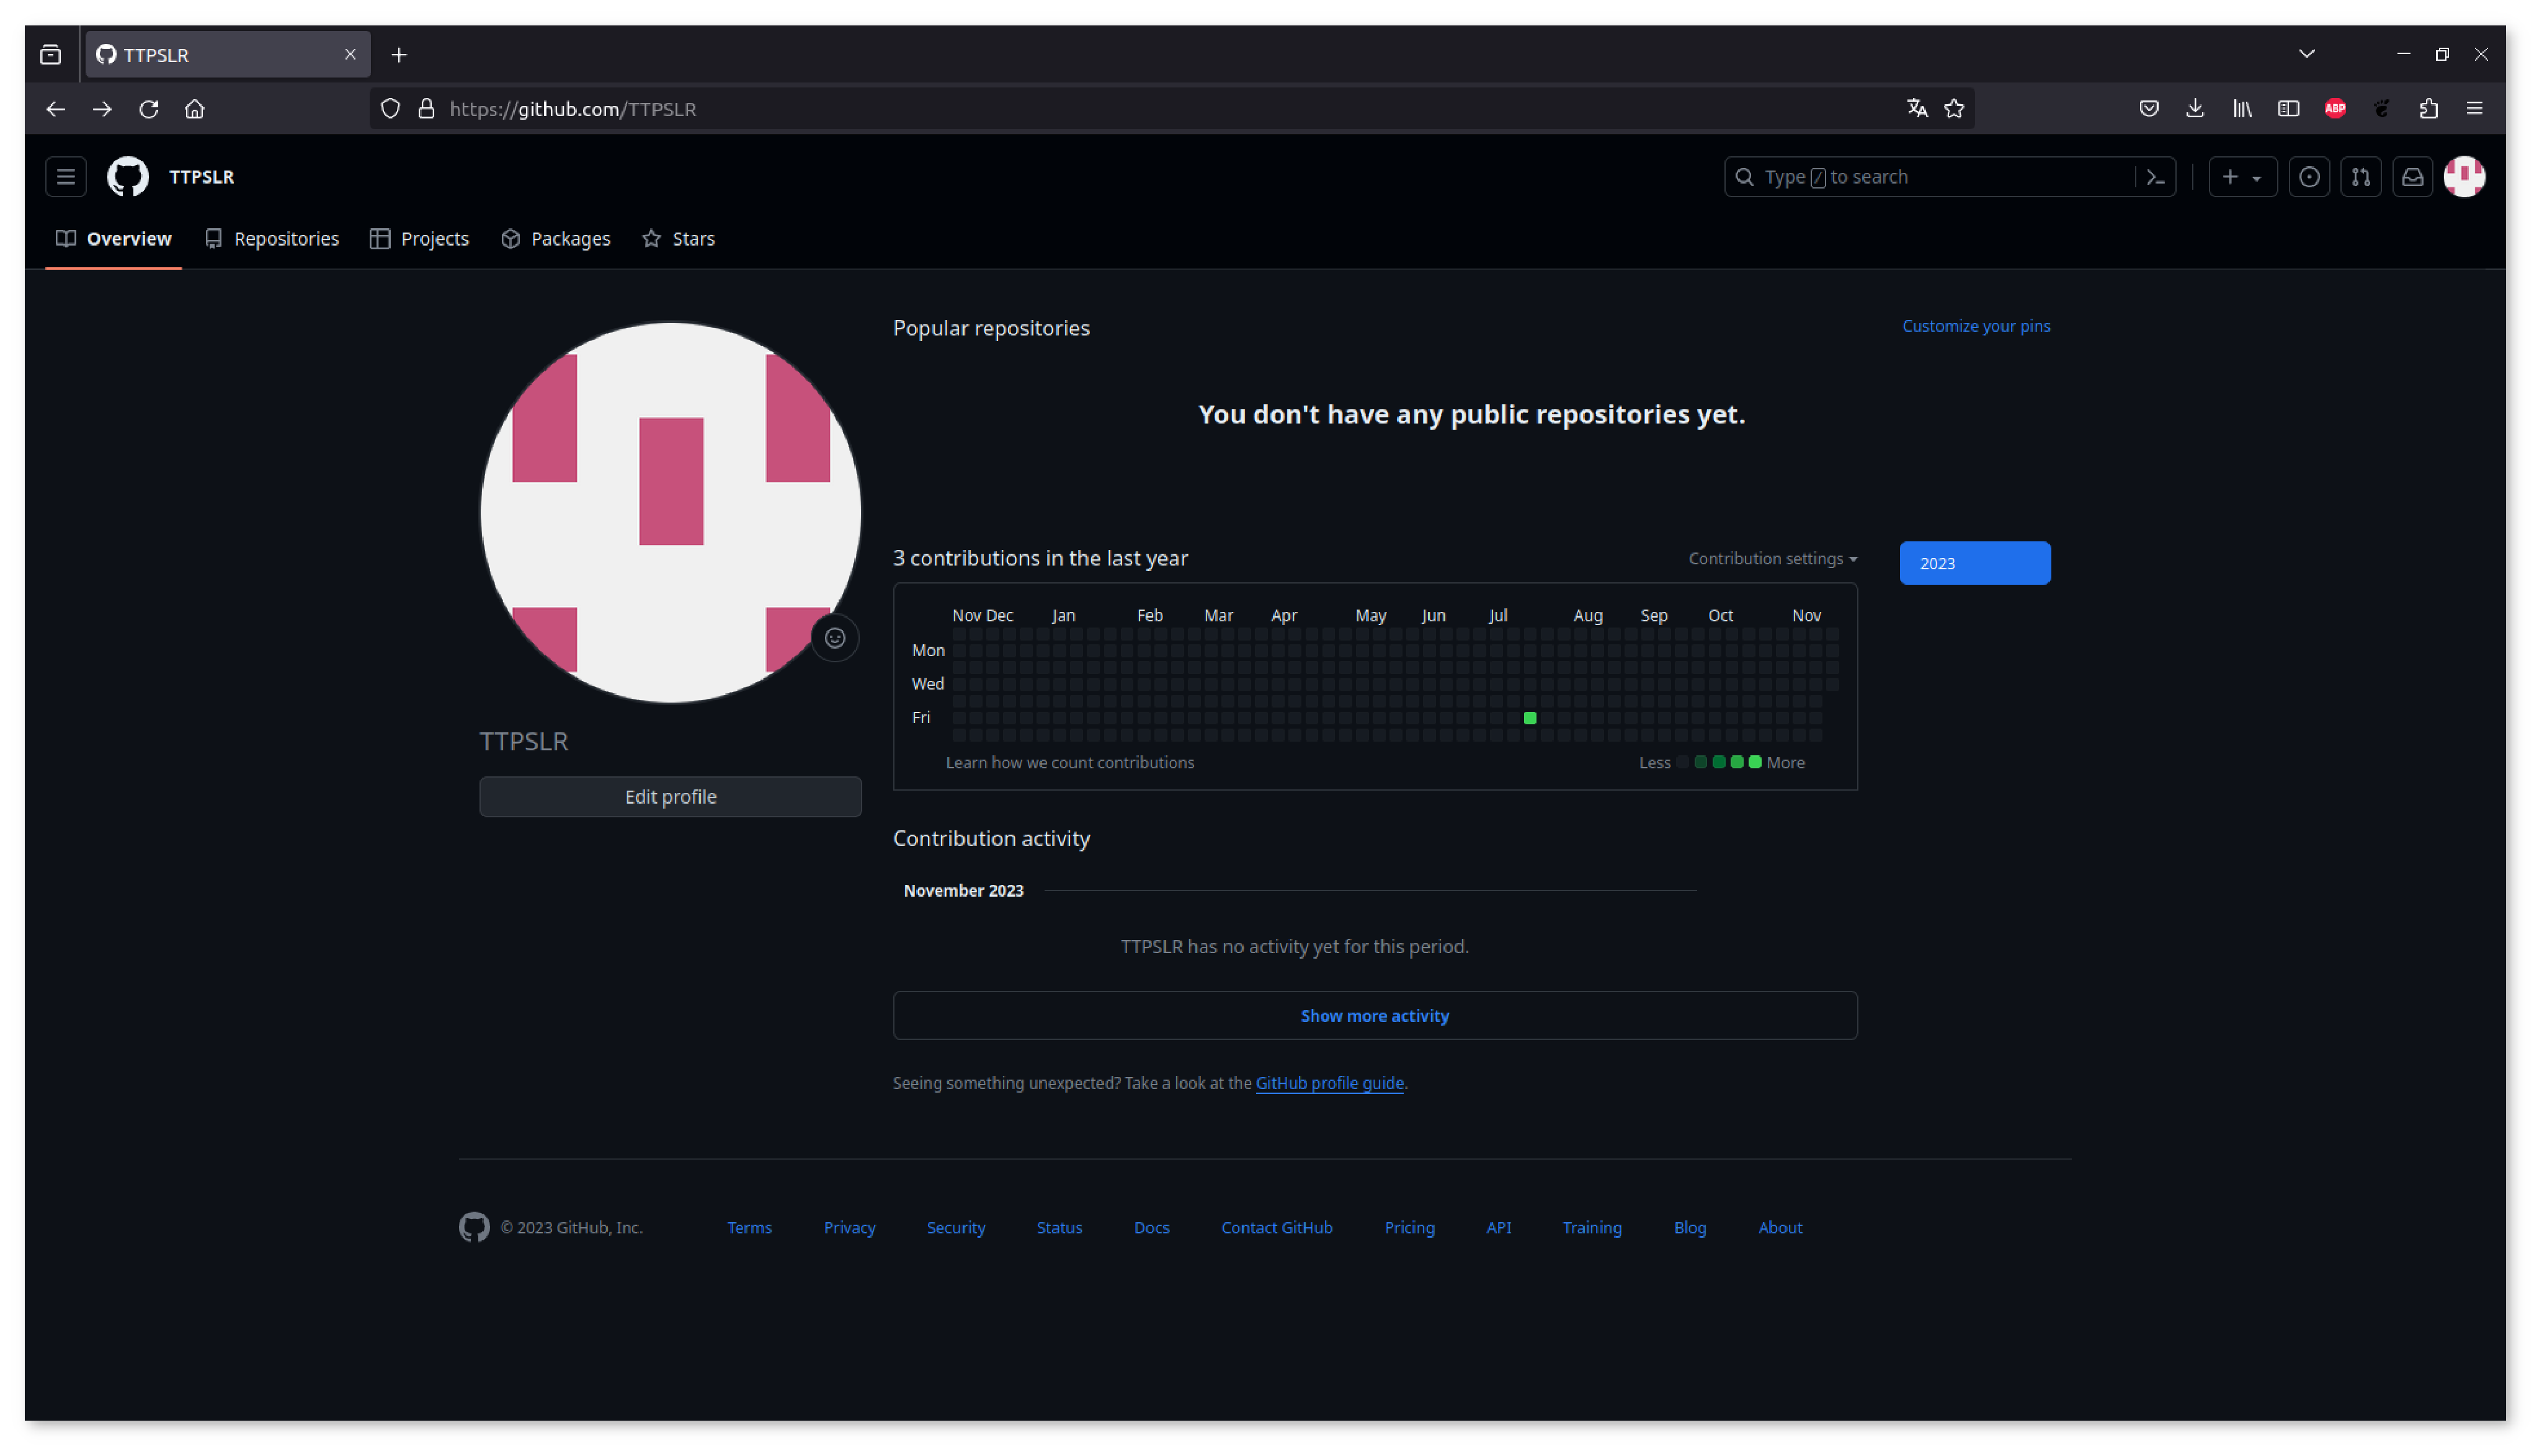
\includegraphics[width=0.85\textwidth,keepaspectratio=true,draft=\ddst]{img/hosts/github/home.eps}
\item \gitlab: \\[0.25cm]
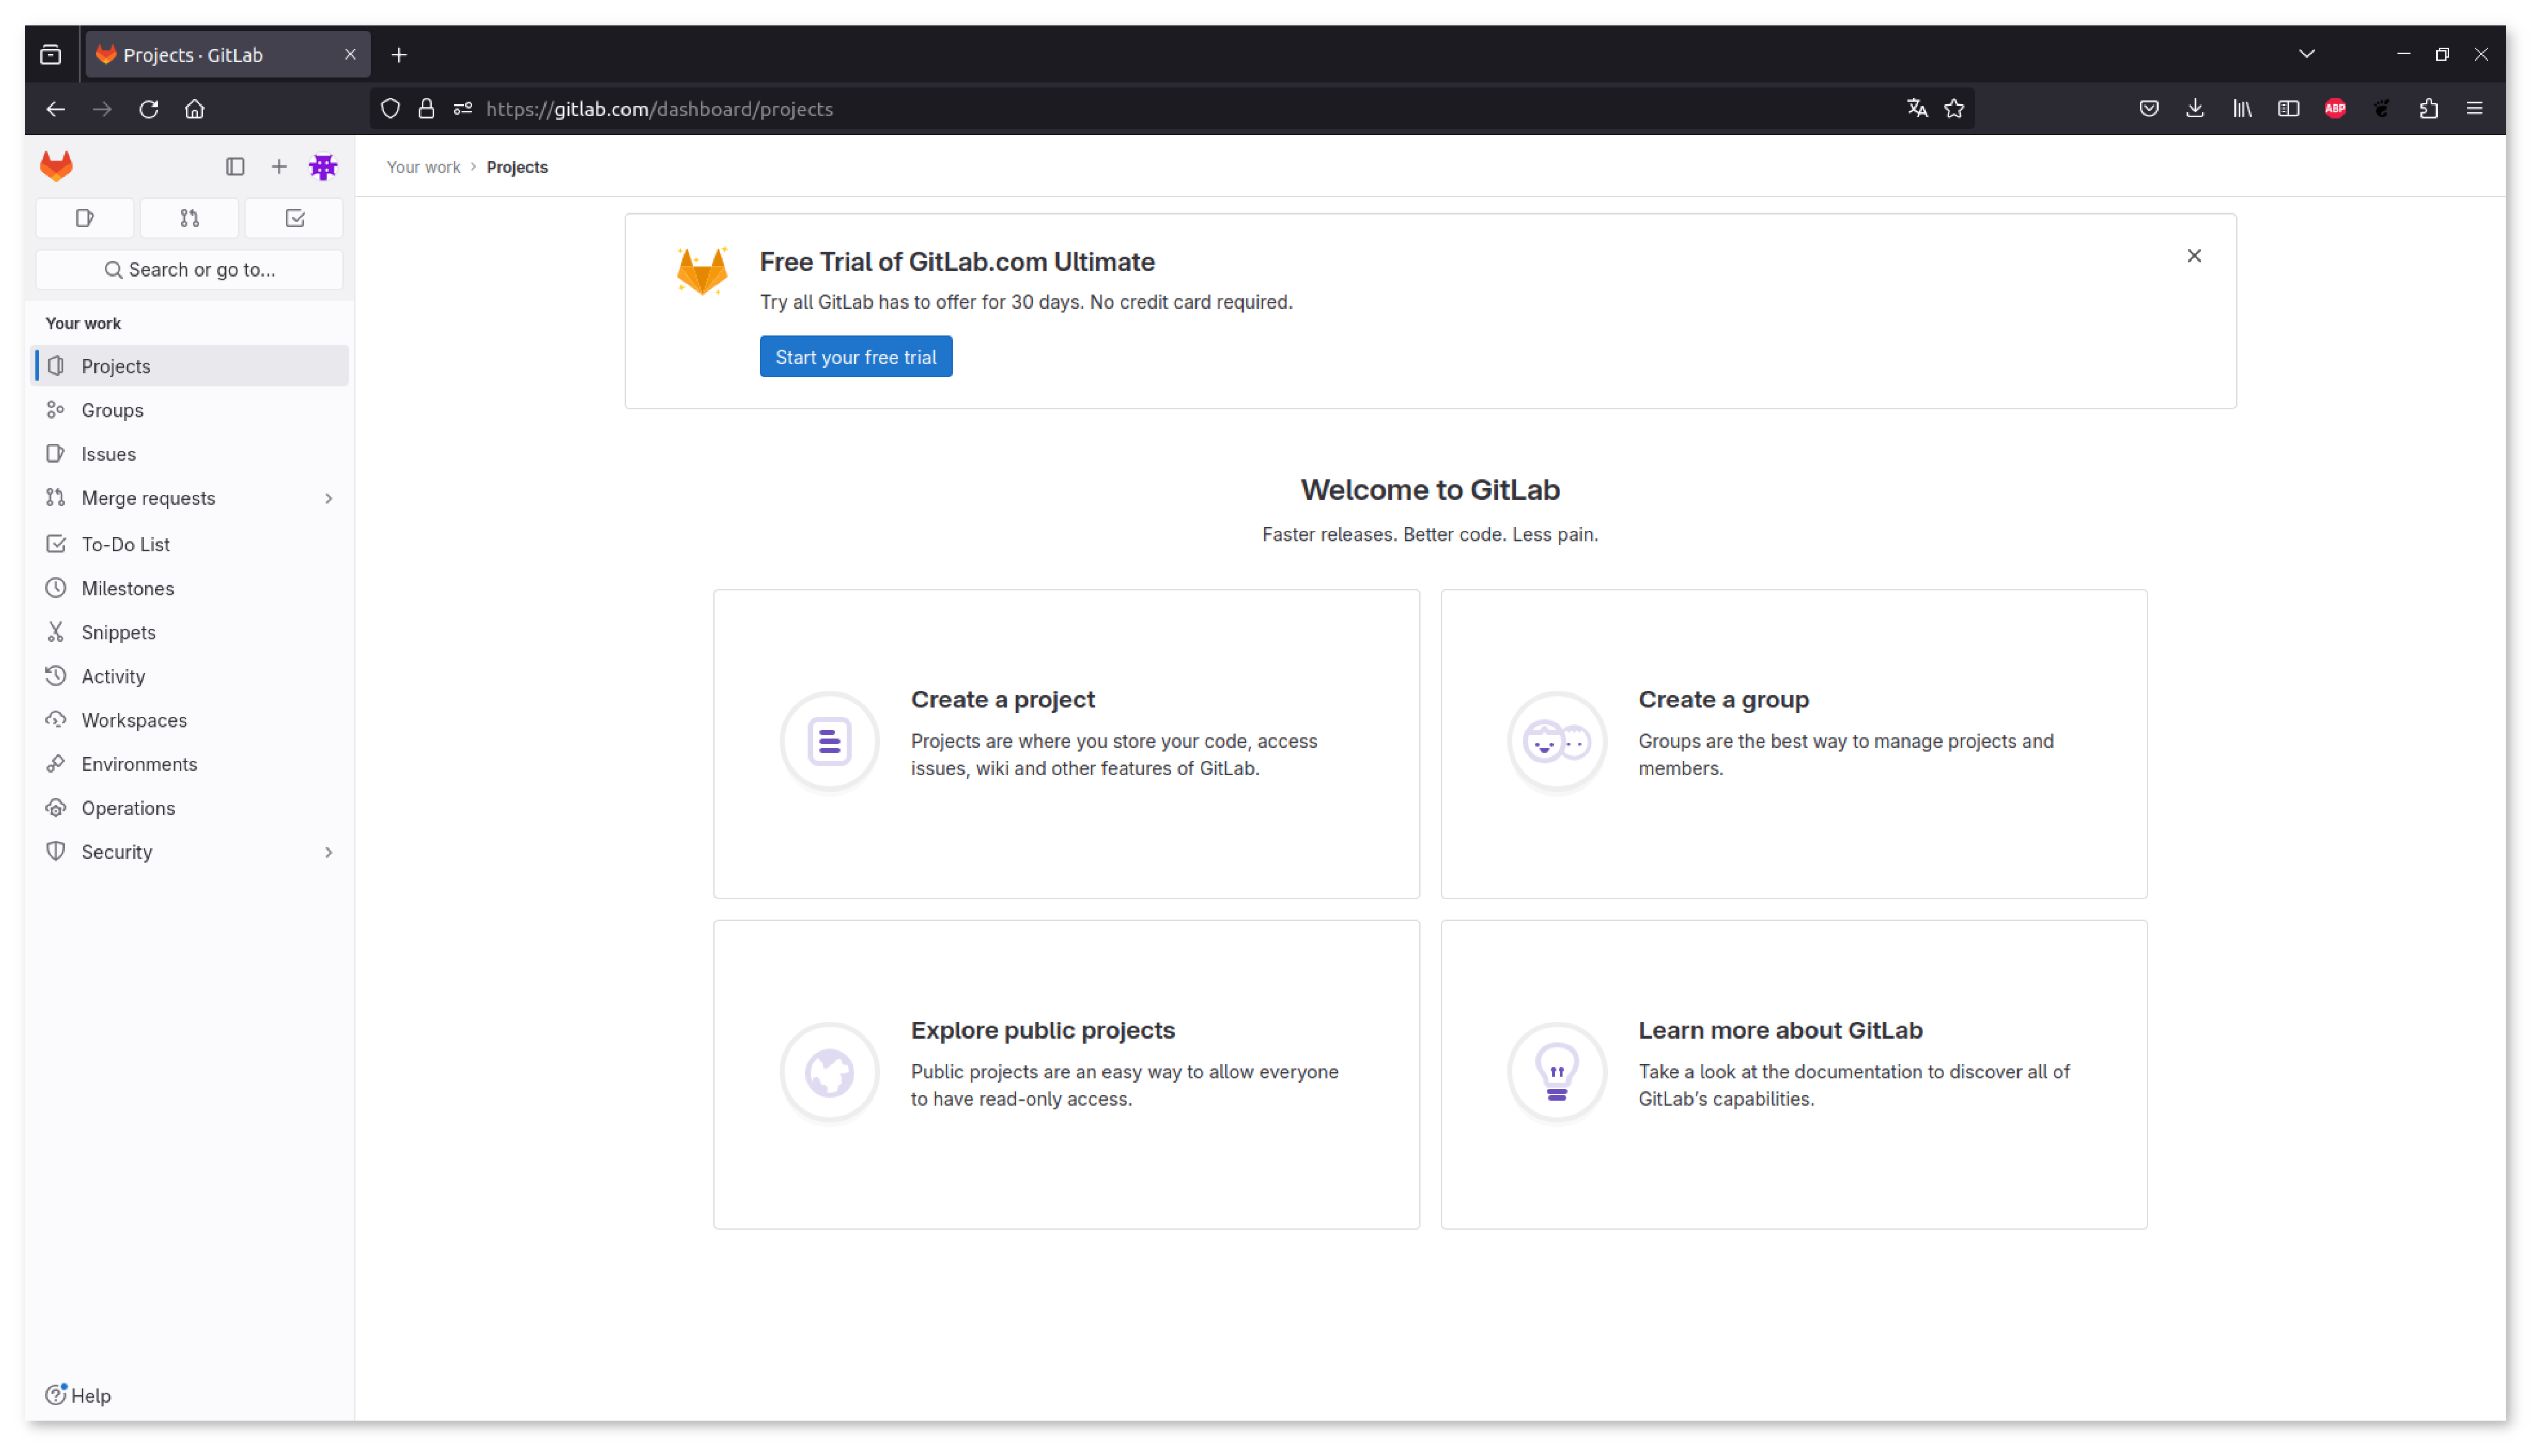
\includegraphics[width=0.85\textwidth,keepaspectratio=true,draft=\ddst]{img/hosts/gitlab/home.eps}
\end{itemize}
In the following examples for both \github\ and \gitlab:
\begin{itemize}
\item the account/group name is: "\texttt{TTPSLR}"
\item the project name is: "\texttt{Program}"
\end{itemize}

\newpage
\section{Creating a repository / project}

The procedure is quite similar, only the denomination changes: 
\begin{itemize}
\item On \github\ the space to store and share your sources is called a "\texttt{repository}"
\item On \gitlab\ the space to store and share your sources is called a "\texttt{project}"
\end{itemize}
\vspace{0.25cm}
\begin{itemize}
\item \github:
\end{itemize}
\vspace{0.5cm}
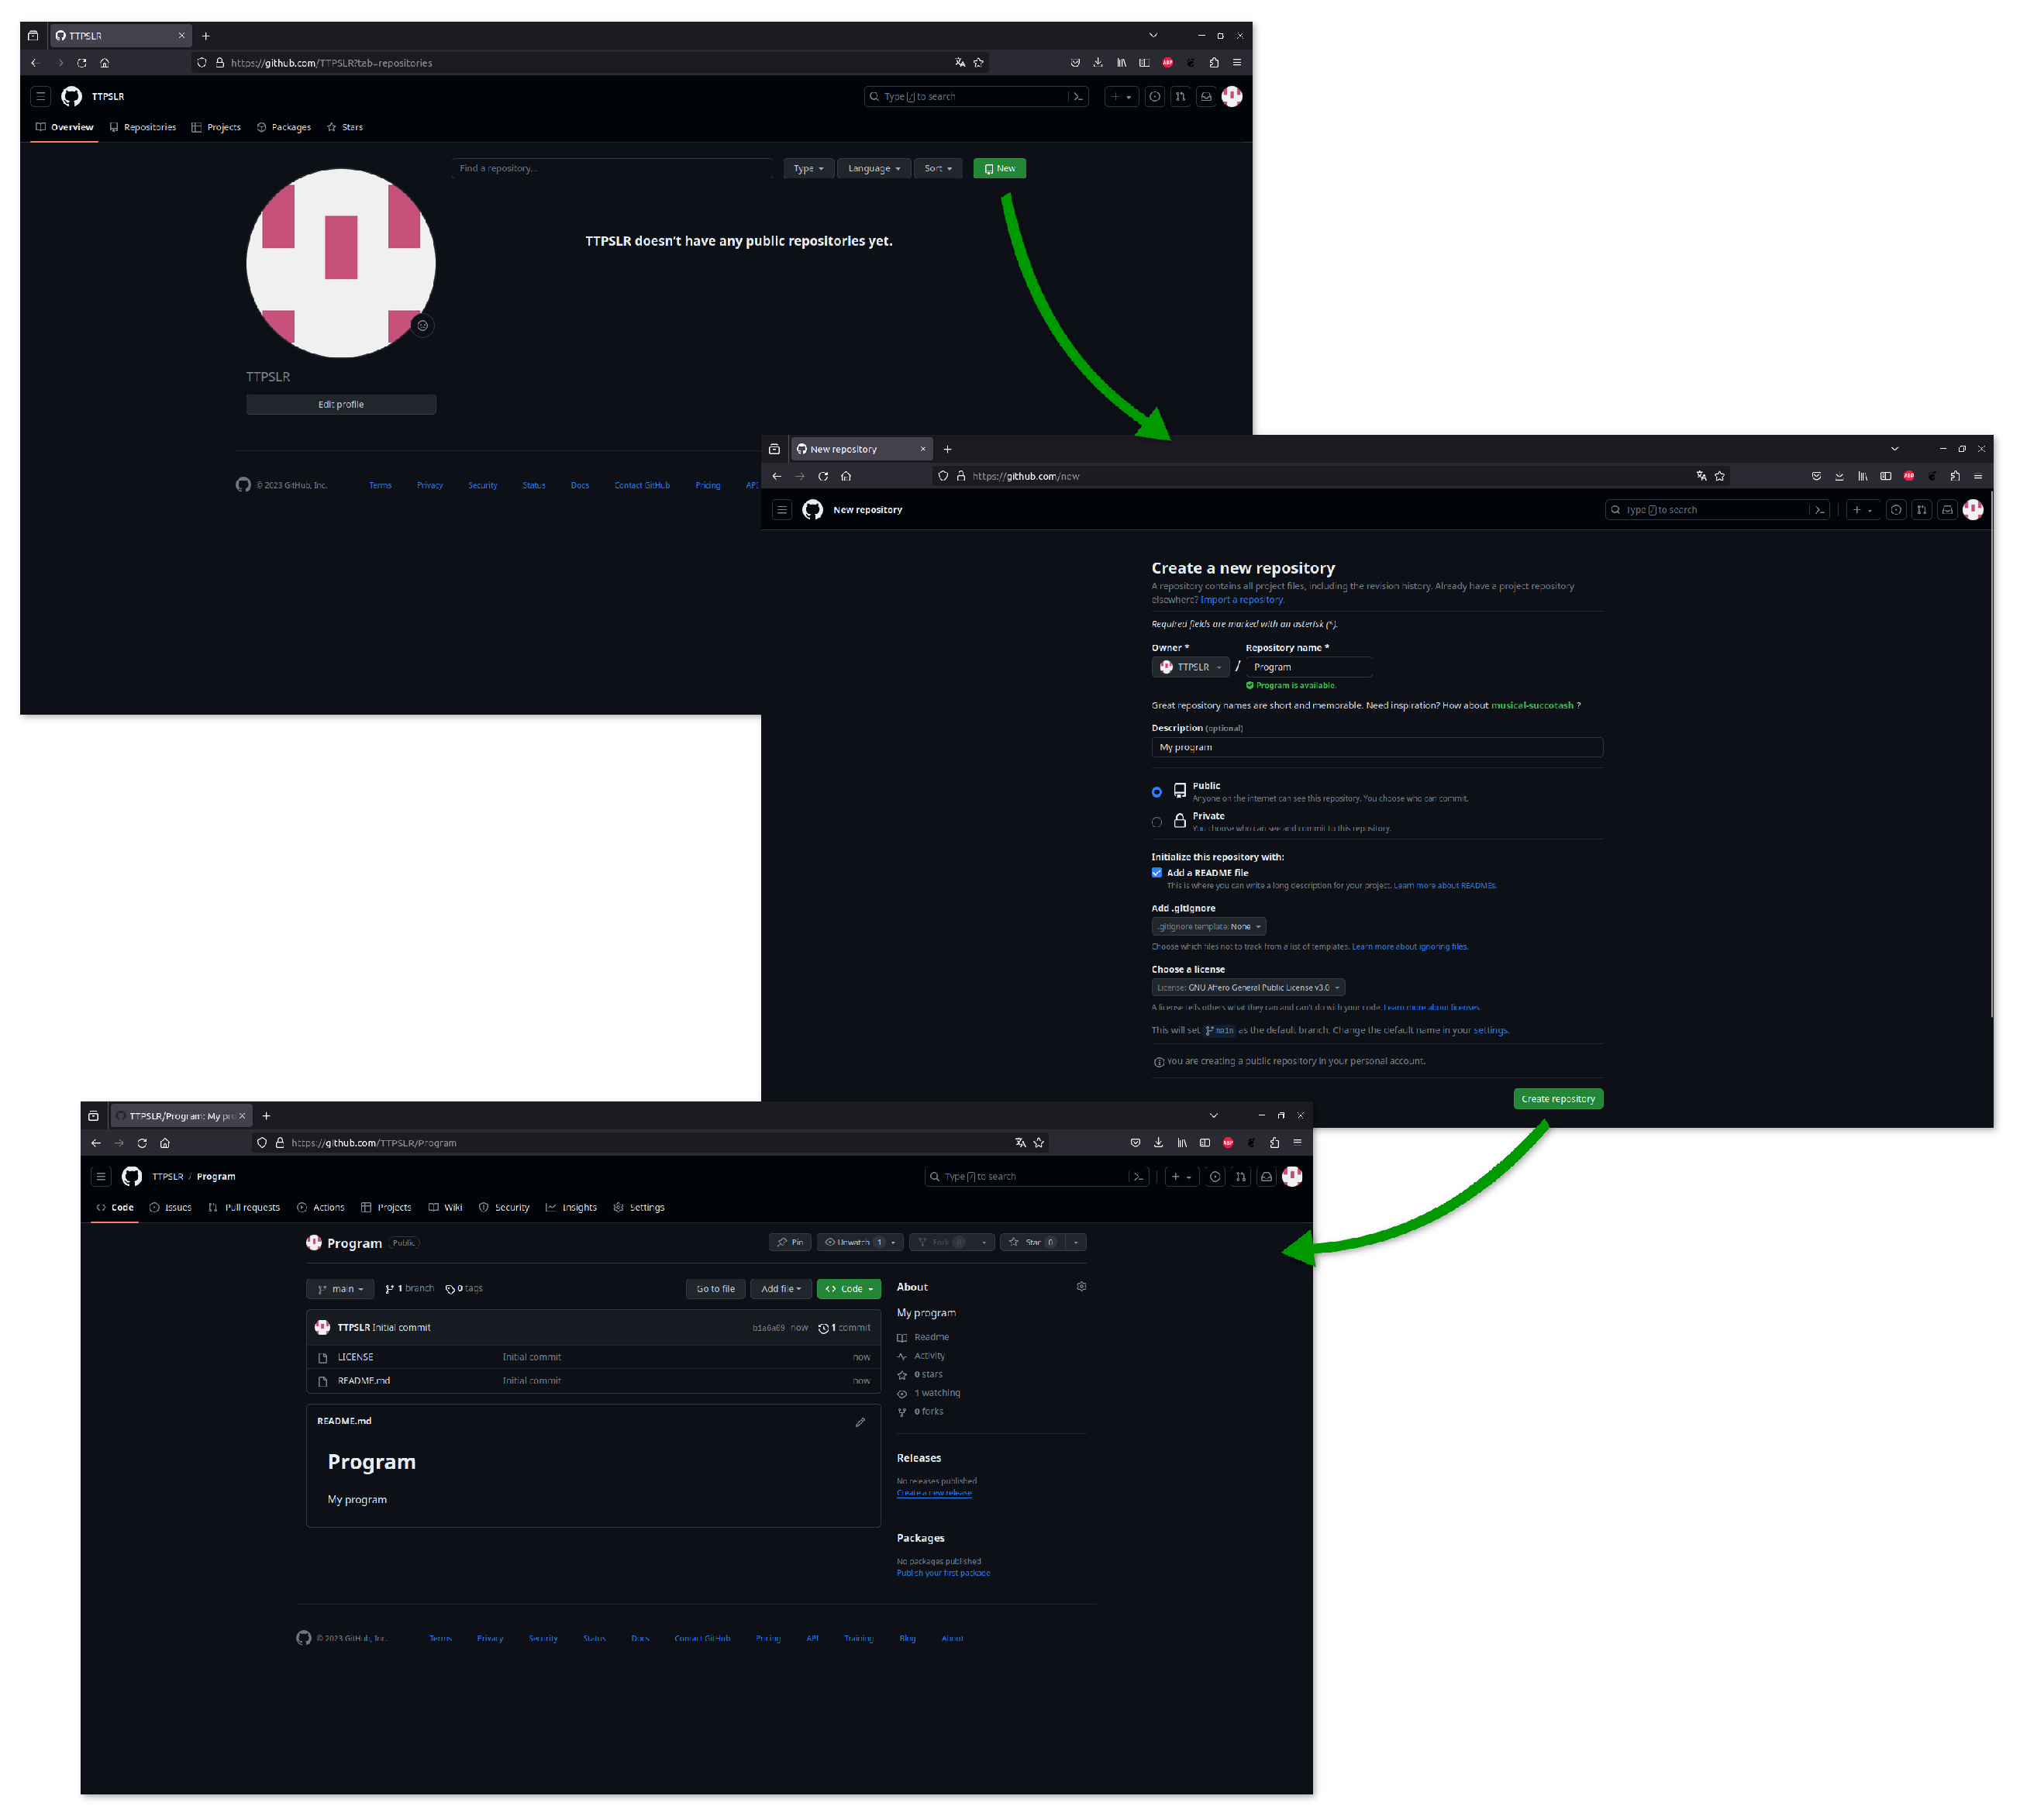
\includegraphics[width=1.0\textwidth,keepaspectratio=true,draft=\ddst]{img/hosts/github/new-p.eps} \\[0.25cm]
\begin{itemize}
\item Open the "\texttt{Repositories}" tab and click on "\texttt{New}"
\item Fill the new project information
\item Click on "\texttt{Create repository}"
\end{itemize}
\newpage
\begin{itemize}
\item \gitlab:
\end{itemize}
\vspace{0.5cm}
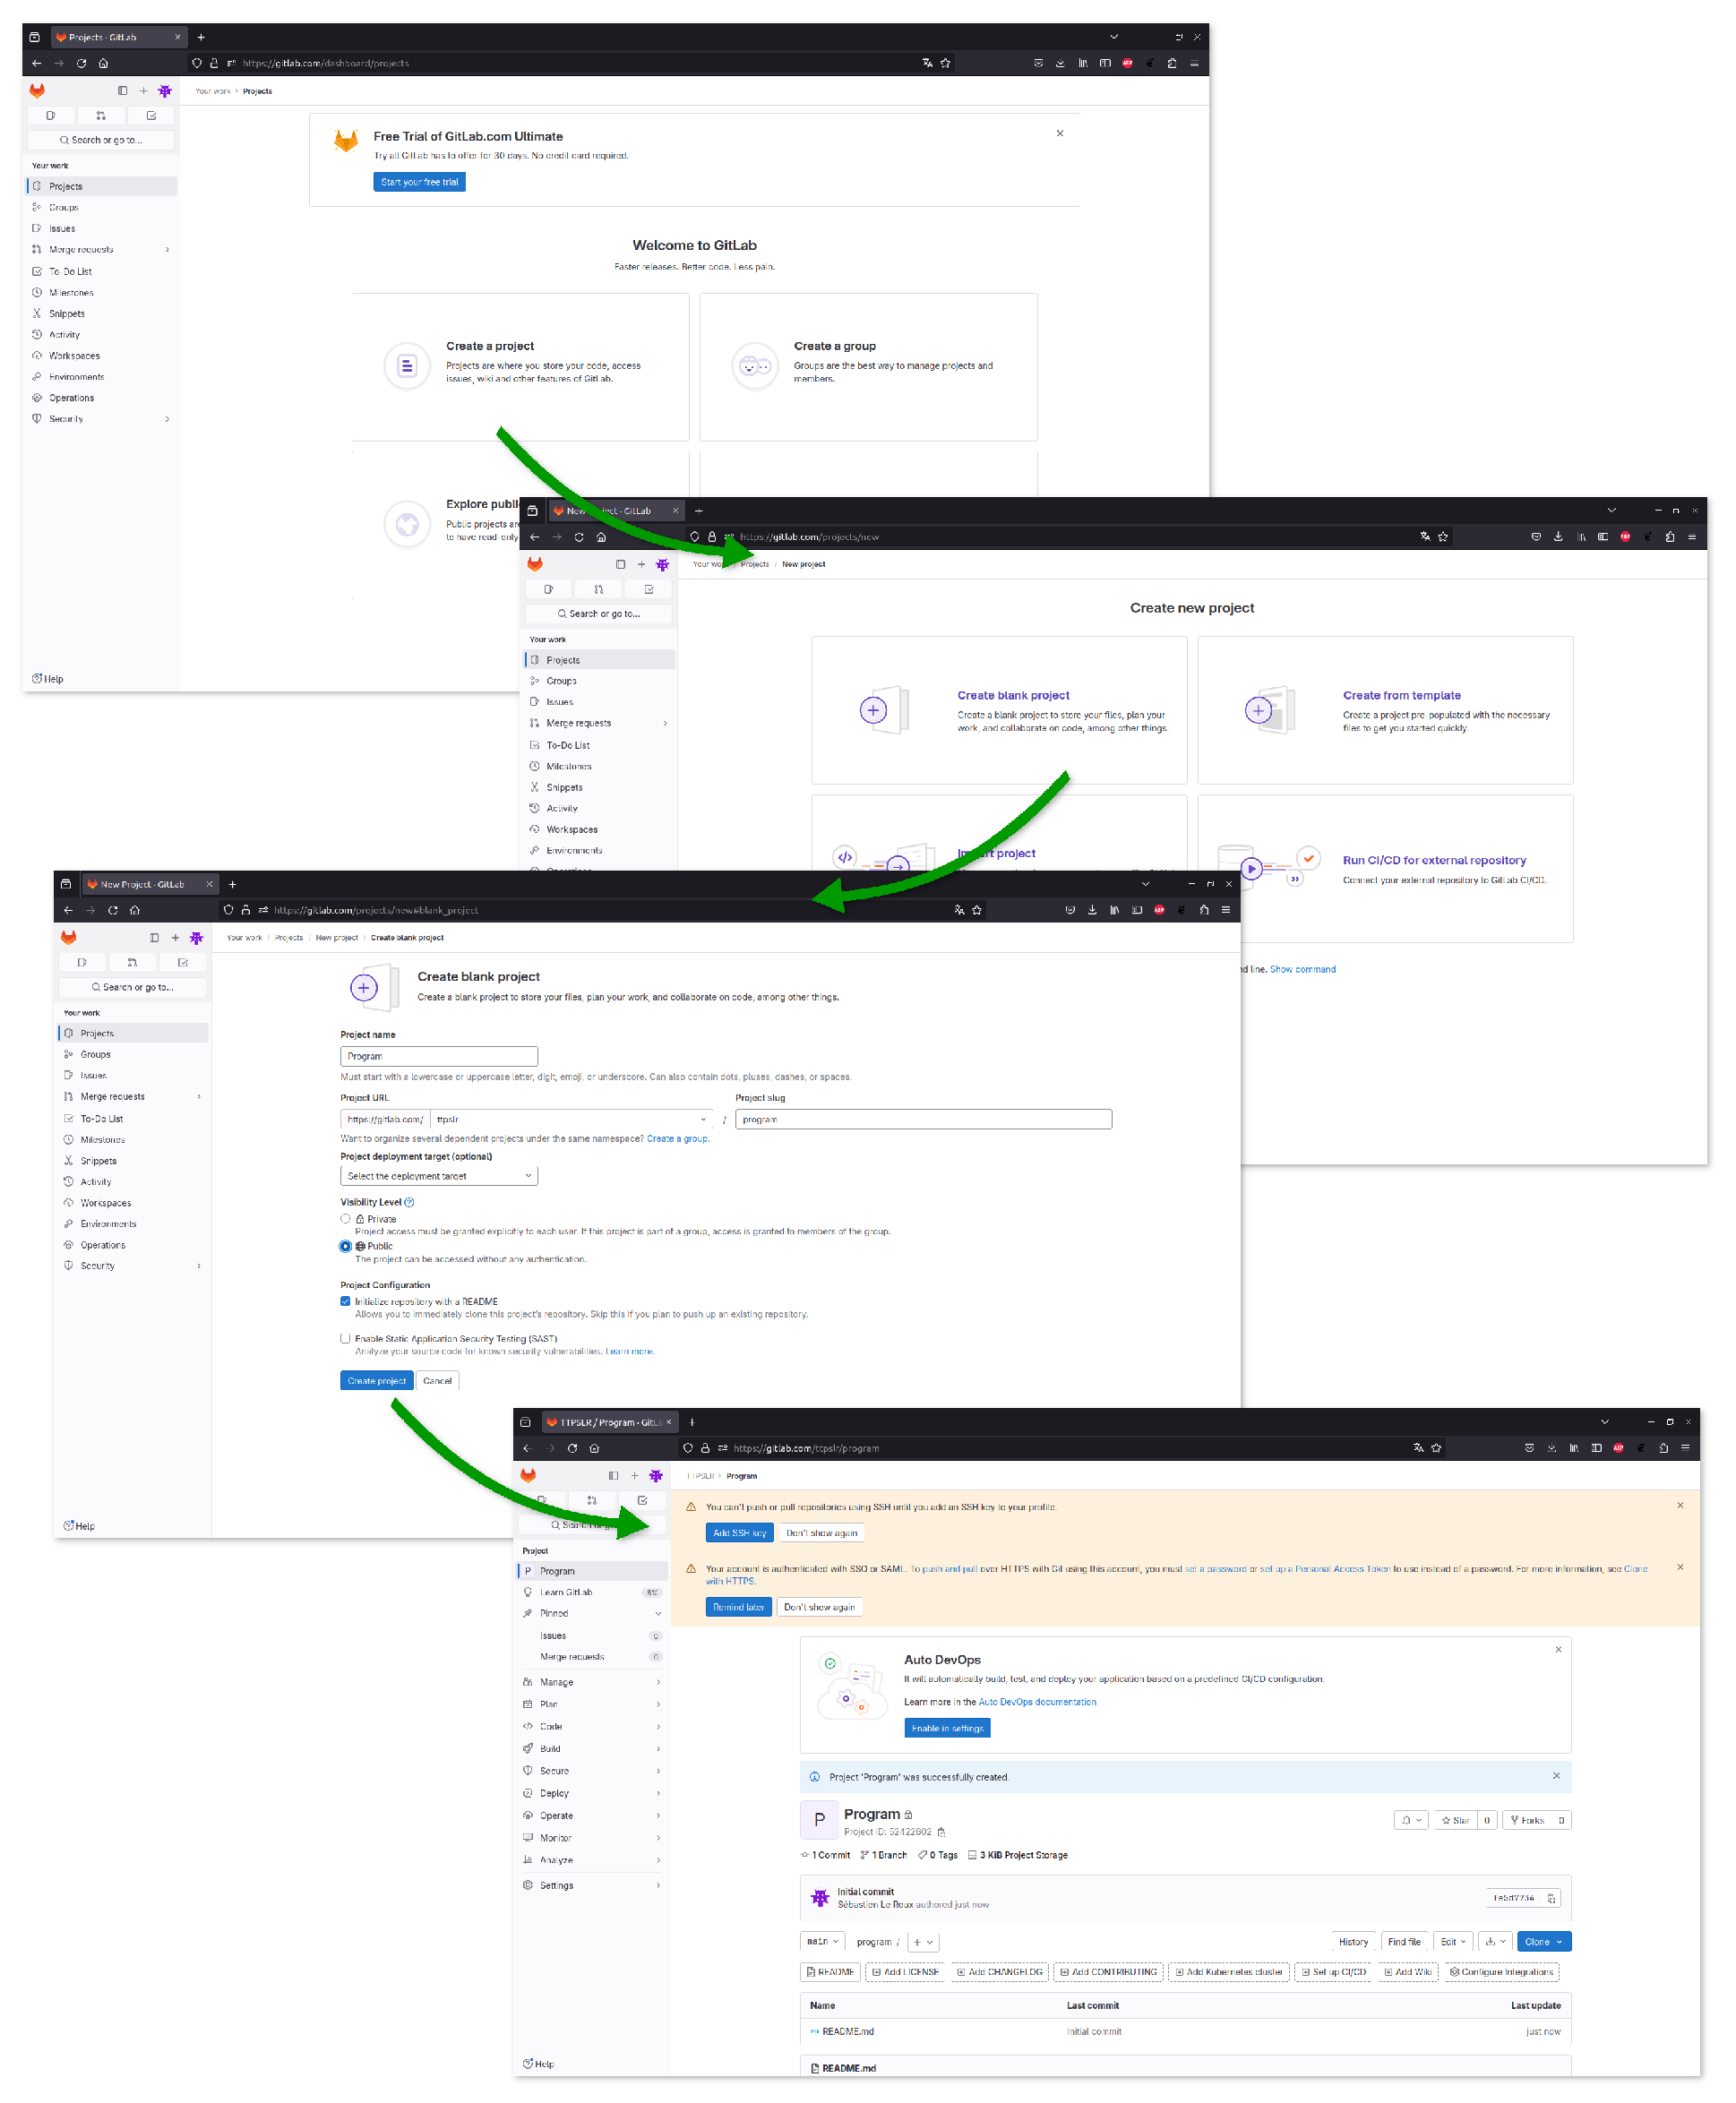
\includegraphics[width=1.0\textwidth,keepaspectratio=true,draft=\ddst]{img/hosts/gitlab/new-p.eps} %\\[0.25cm]
\newpage
\begin{itemize}
\item Click on "\texttt{Create project}"
\item Click on "\texttt{Create blank project}"
\item Fill the new project information
\item Click on "\texttt{Create project}"
\end{itemize}

\section{SSH encryption keys}

Immediately after creating your first project, setup the SSH encryption keys. 
These keys are digital tokens that prove your identity when performing actions to update the on line repository using Git. 

\subsection{Generating SSH encryption keys}

If not done already you need first to create SSH encryption keys, this is done using a command line utility: 
\begin{script}
\fprompt{~} \bftt{ssh-keygen} \rtt{-t} \dgtt{ed25519}
\end{script}
"\bftt{ssh-keygen}" generates the key, the "\rtt{-t}" option is used to define the type of encoding, in the example "\dgtt{ed25519}" that stands for \href{https://en.wikipedia.org/wiki/EdDSA}{Edwards-curve Digital Signature Algorithm} which is the most secured standardization these days.  \\
2 files, to be stored in "\texttt{\textasciitilde/.ssh}", will be created by the previous command:
\begin{itemize}
\item A private key, that decipher (act like a key), and that must remains on your computer: 
\begin{scripti}
~/.ssh/id\_ed25519
\end{scripti} \\
\vspace{-1.5cm}
\item A matching public key, that encrypts (acts like a door), used on remote system(s):
\begin{scripti}
~/.ssh/id\_ed25519.pub
\end{scripti} \\[-0.65cm]
\noindent Which content looks like: 
{\scriptsize{
\begin{scripti}
\fprompt{~} cat ~/.ssh/id\_ed25519.pub
ssh-ed25519 AAAAC3NzaC1lZDI1NTE5AAAAIG1TIYyaRZIlFU40NH8QAxXK8SSgl07Thop6CGzcVg0j user@host
\end{scripti}}} \\
\vspace{-1.5cm}
\end{itemize}
For more about asymmetric keys algorithms: \href{https://en.wikipedia.org/wiki/Public-key\_cryptography}{https://en.wikipedia.org/wiki/Public-key\_cryptography}
\newpage

\subsection{Adding the keys to GitHub / GitLab}

Now you need to add the public key to your \github\ / \gitlab\ repository: 
\begin{itemize}
\item \github\ (see figure~\ref{kgithub}):
\begin{itemize}
\item Click on the profile logo and click on "\texttt{Settings}"
\item Click on the "\texttt{SSH and GPG keys}"
\item Click on "\texttt{Create repository}"
\item Click on "\texttt{New SSH key}"
\item Adjust the key information:
\begin{itemize}
\item Give the key a title name
\item Select the key type: "\texttt{Authentication key}" 
\item Copy / paste the content of public key file in the text box
\end{itemize}
\item Finally click on "\texttt{Add SSH key}"
\end{itemize}
\item \gitlab\ (see figure~\ref{kgitlab}):
\begin{itemize}
\item Click on shortcut button "\texttt{Add SSH key}" \\
Alternatively click on your public avatar (squared in red in figure~\ref{kgitlab}), \\
click on "\texttt{Preferences}", then click on "\texttt{SSH Keys}"
\item Click on the "\texttt{Add new key}"
\item Adjust the key information:
\begin{itemize}
\item Copy / paste the content of public key file in the text box
\item Give the key a title name
\item Select the key type: "\texttt{Authentication}" or "\texttt{Authentication \& Signing}" 
\end{itemize}
\item Finally click on "\texttt{Add key}"
\item Optionally go back the "\texttt{User Settings} $\Longrightarrow$ \texttt{SSH Keys}" tab to visualize that the key is properly stored
\end{itemize}
\end{itemize}
As soon as the keys have been installed you are ready to work with your on line repository. 

\begin{figure}[!p]
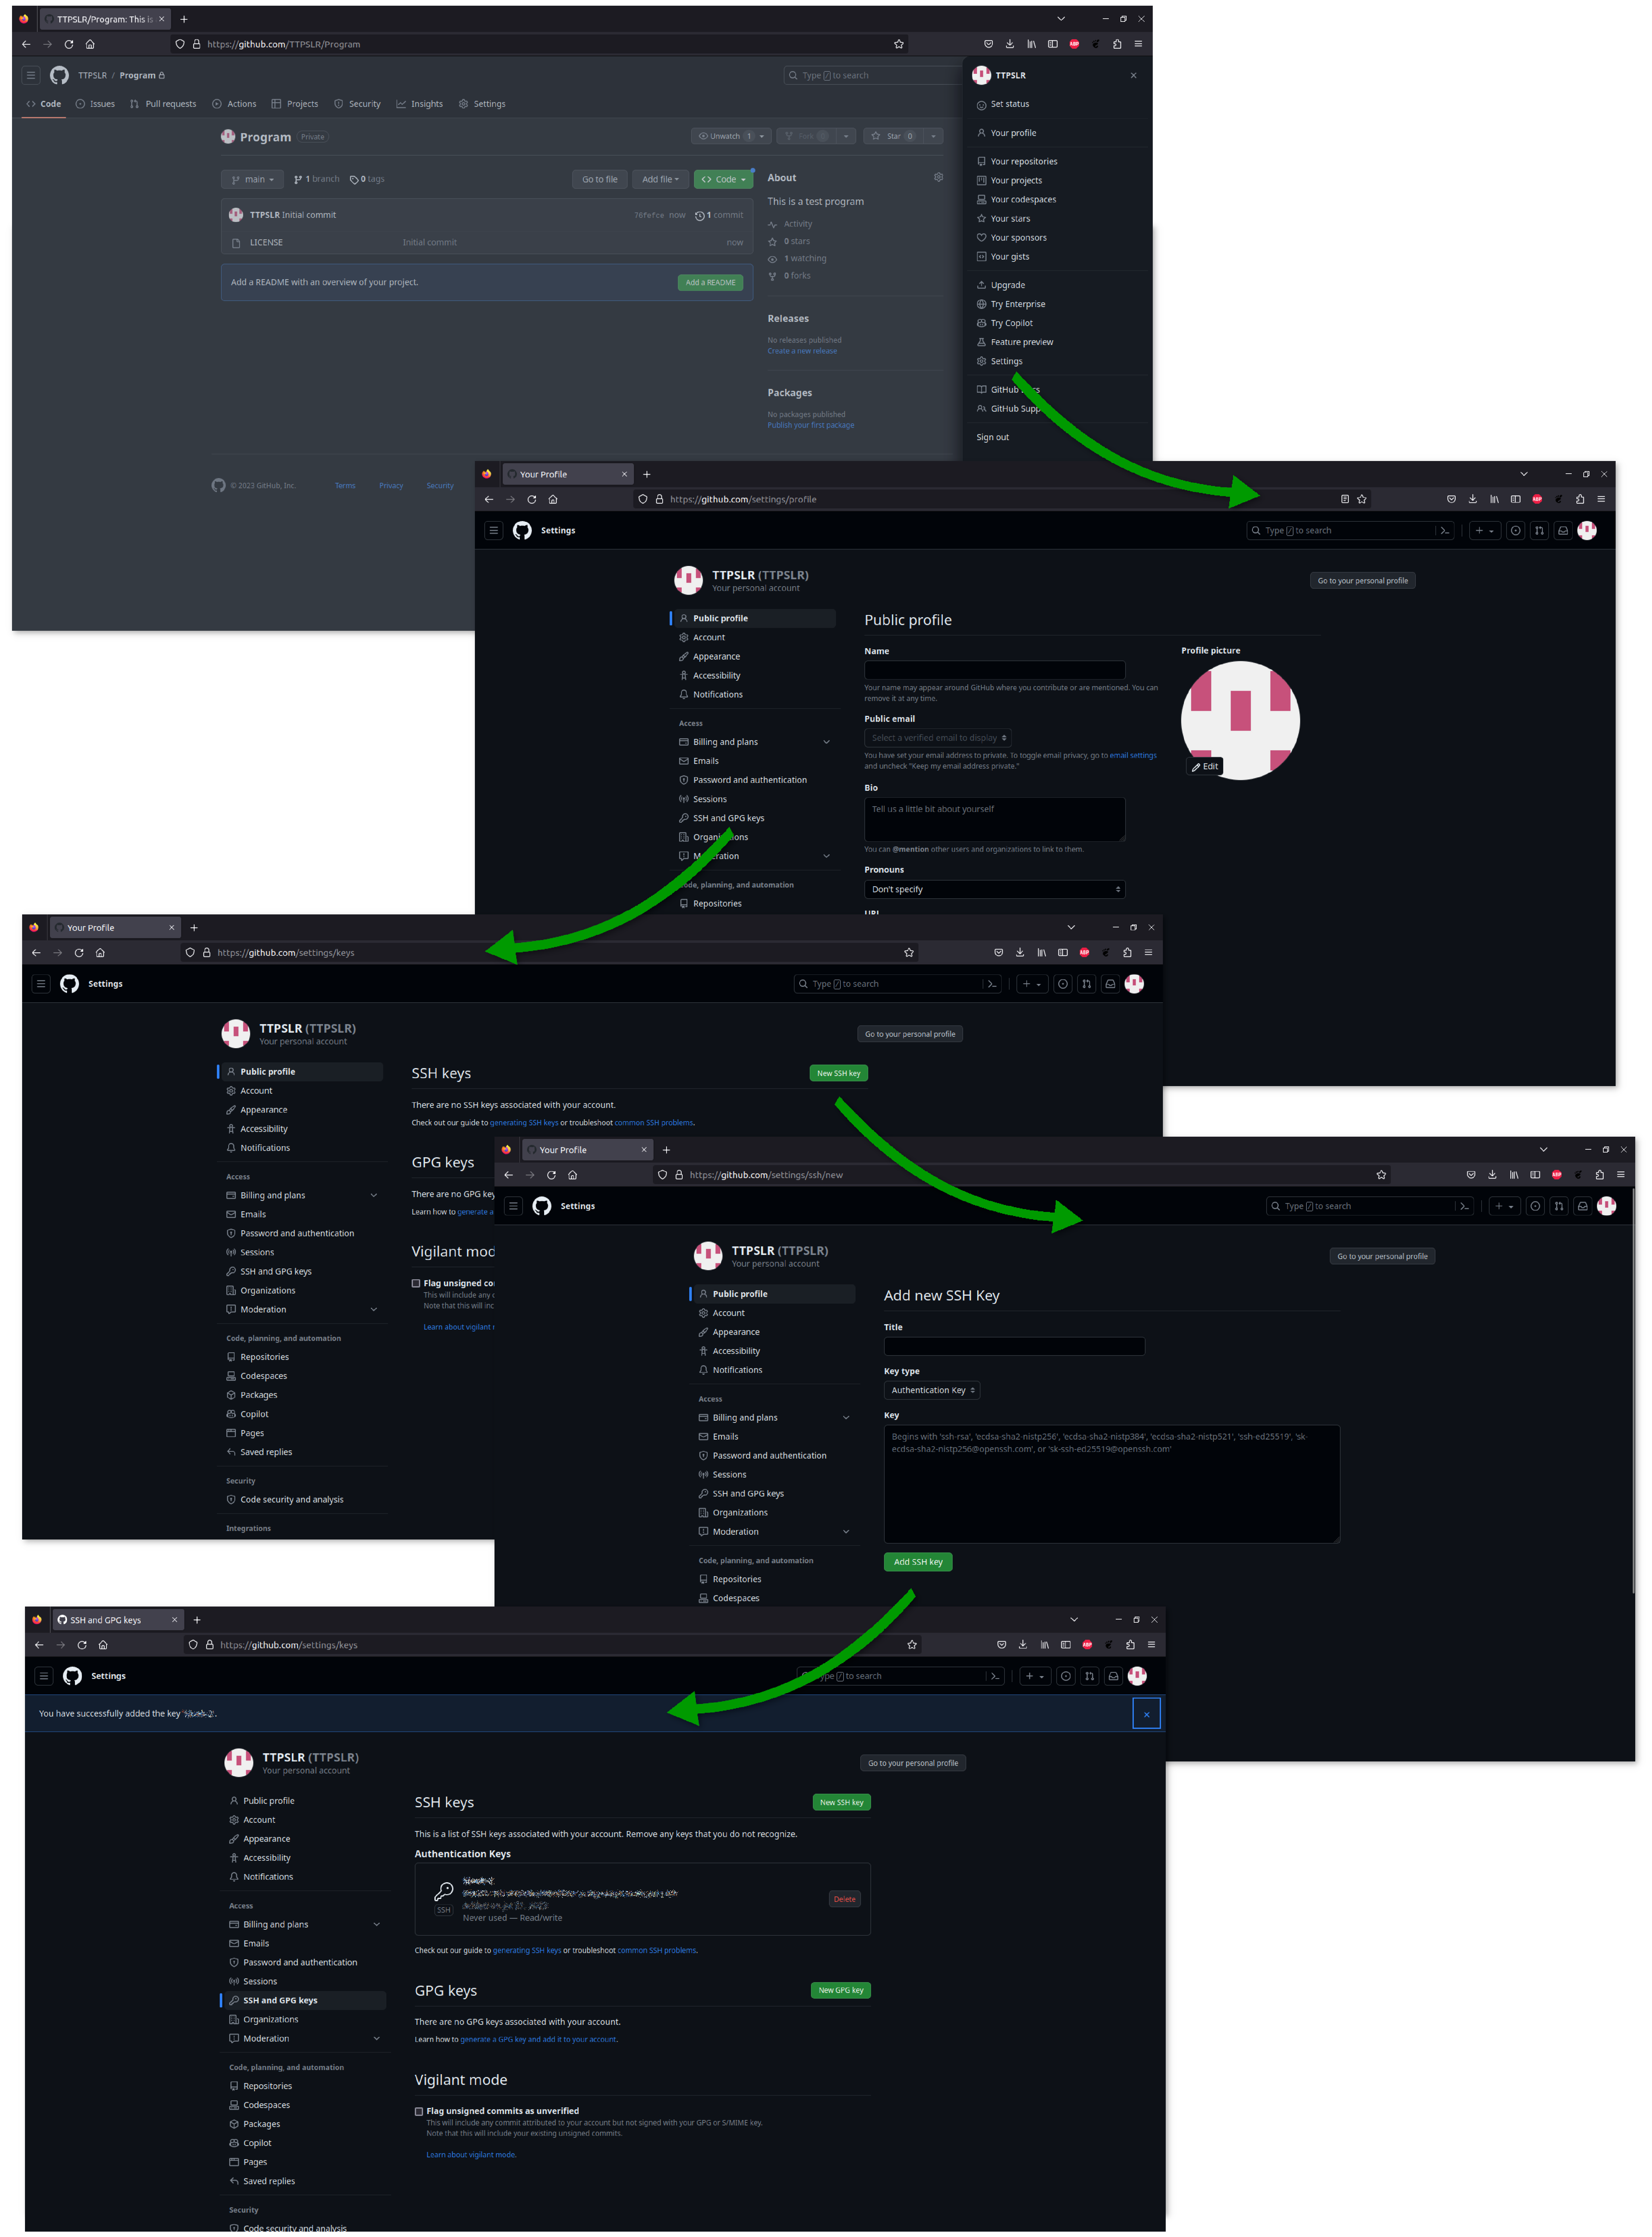
\includegraphics[width=1.0\textwidth,keepaspectratio=true,draft=\ddst]{img/hosts/github/keys.eps} 
\caption{Adding a SSH key on \github\label{kgithub}}
\end{figure}

\begin{figure}[!p]
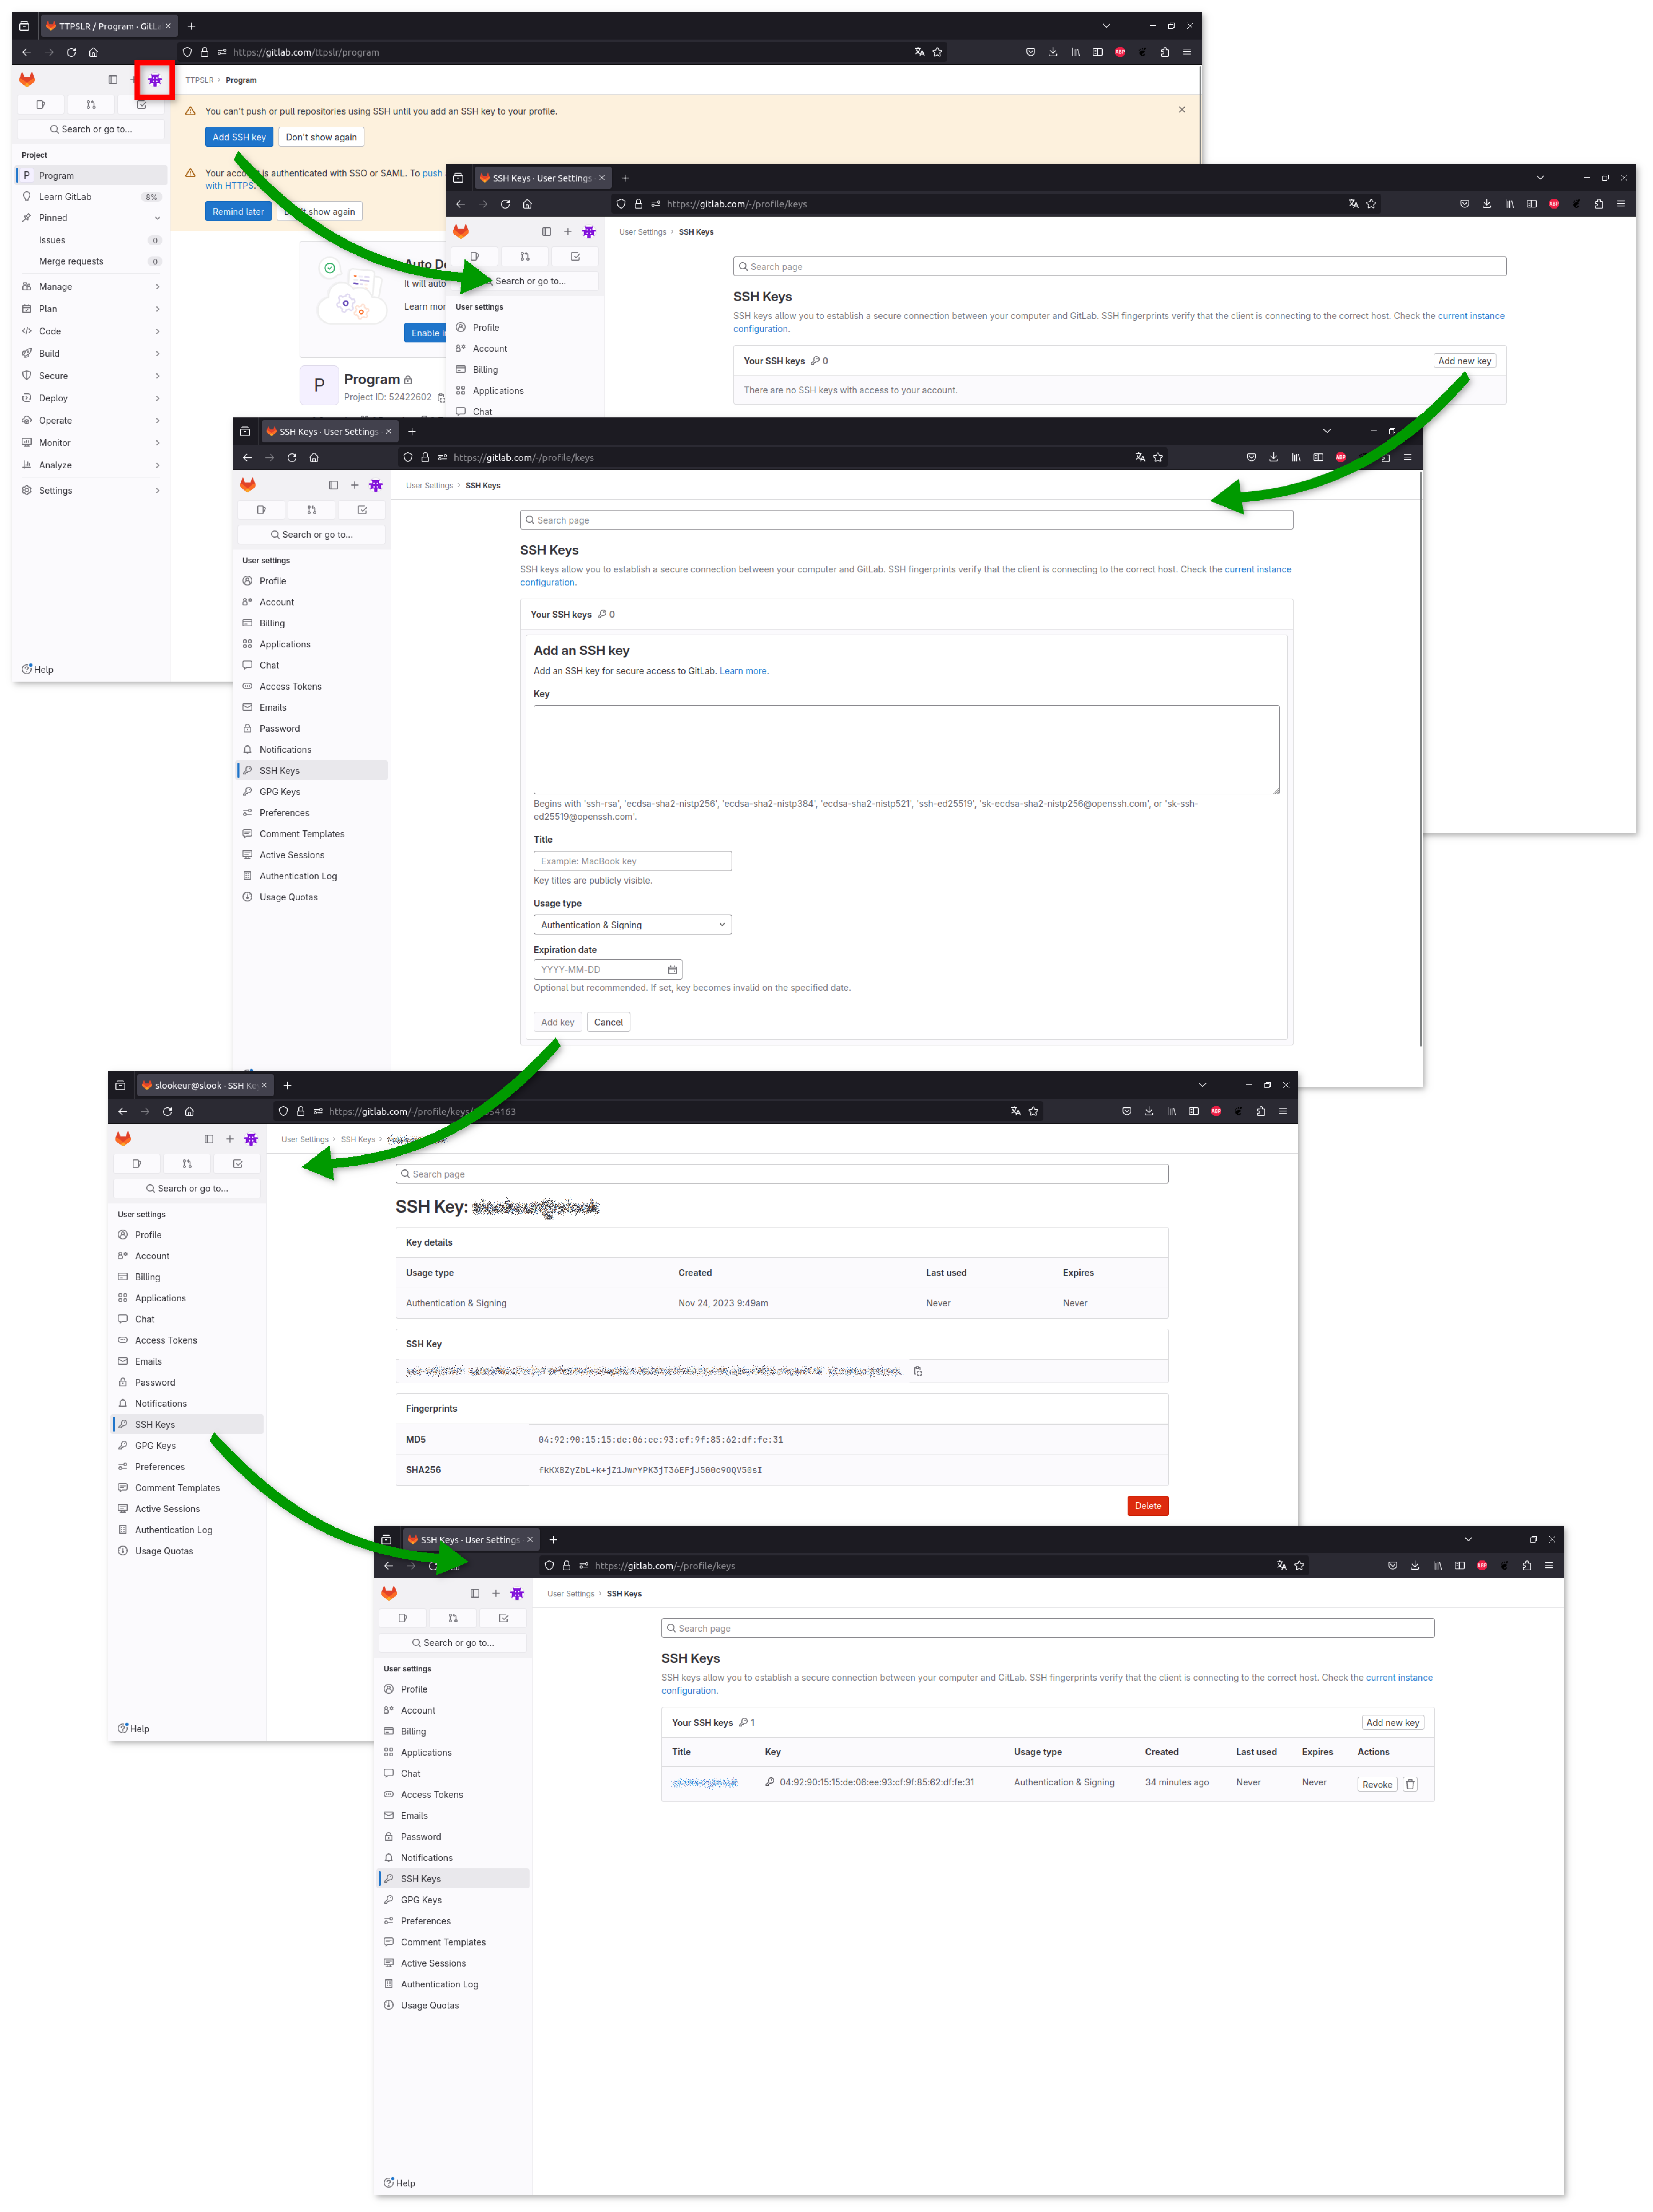
\includegraphics[width=1.0\textwidth,keepaspectratio=true,draft=\ddst]{img/hosts/gitlab/keys.eps} 
\caption{Adding a SSH key on \gitlab\label{kgitlab}}
\end{figure}

\clearpage

\section{Branch protection}

If you are managing collaborative project, with several developers being able to push commits to the Git (and \github\ or \gitlab) repository branch(es), 
then you need to ensure that branch(es) of your project is (are) being protected against errors, ensuring that changes are handled by the project manager, or designated and selected developers. \\
To do that you need to enable, and adjust, branch(es) protection:
\begin{itemize}
\item \github\ (see figure~\ref{bgithub}):
\begin{itemize}
\item Click on "\texttt{Settings}"
\item Click on "\texttt{Branches}"
\item Click on "\texttt{Add branch protection rule}"
\item Choose branch name and adjust the protection level for this target branch of your project
\item Scroll down and click on "\texttt{Create}"
\end{itemize}
Note that on \github\ no branch protection is in place at the beginning to this step is really important. 
\item \gitlab:
\begin{itemize}
\item Default main branch protection for all your projects (see figure~\ref{mbgitlab}):
\begin{itemize}
\item Click on "\texttt{Settings}" $\Longrightarrow$ "\texttt{Repository}"
\item In front of "\texttt{Default branch}" click on "\texttt{Expand}"
\item Ensure that "\texttt{Fully protected}" 
\end{itemize}
\item Other branches protection (see figure~\ref{bpgitlab}):
\begin{itemize}
\item Click on "\texttt{Settings}" $\Longrightarrow$ "\texttt{Repository}"
\item In front of "\texttt{Protected branches}" click on "\texttt{Expand}"
\item Adjust the protection level for the target branch of your project
\end{itemize}
\end{itemize}
On \gitlab\ however branch protection should already be in place for the main branch.
\end{itemize}

\begin{figure}[!p]
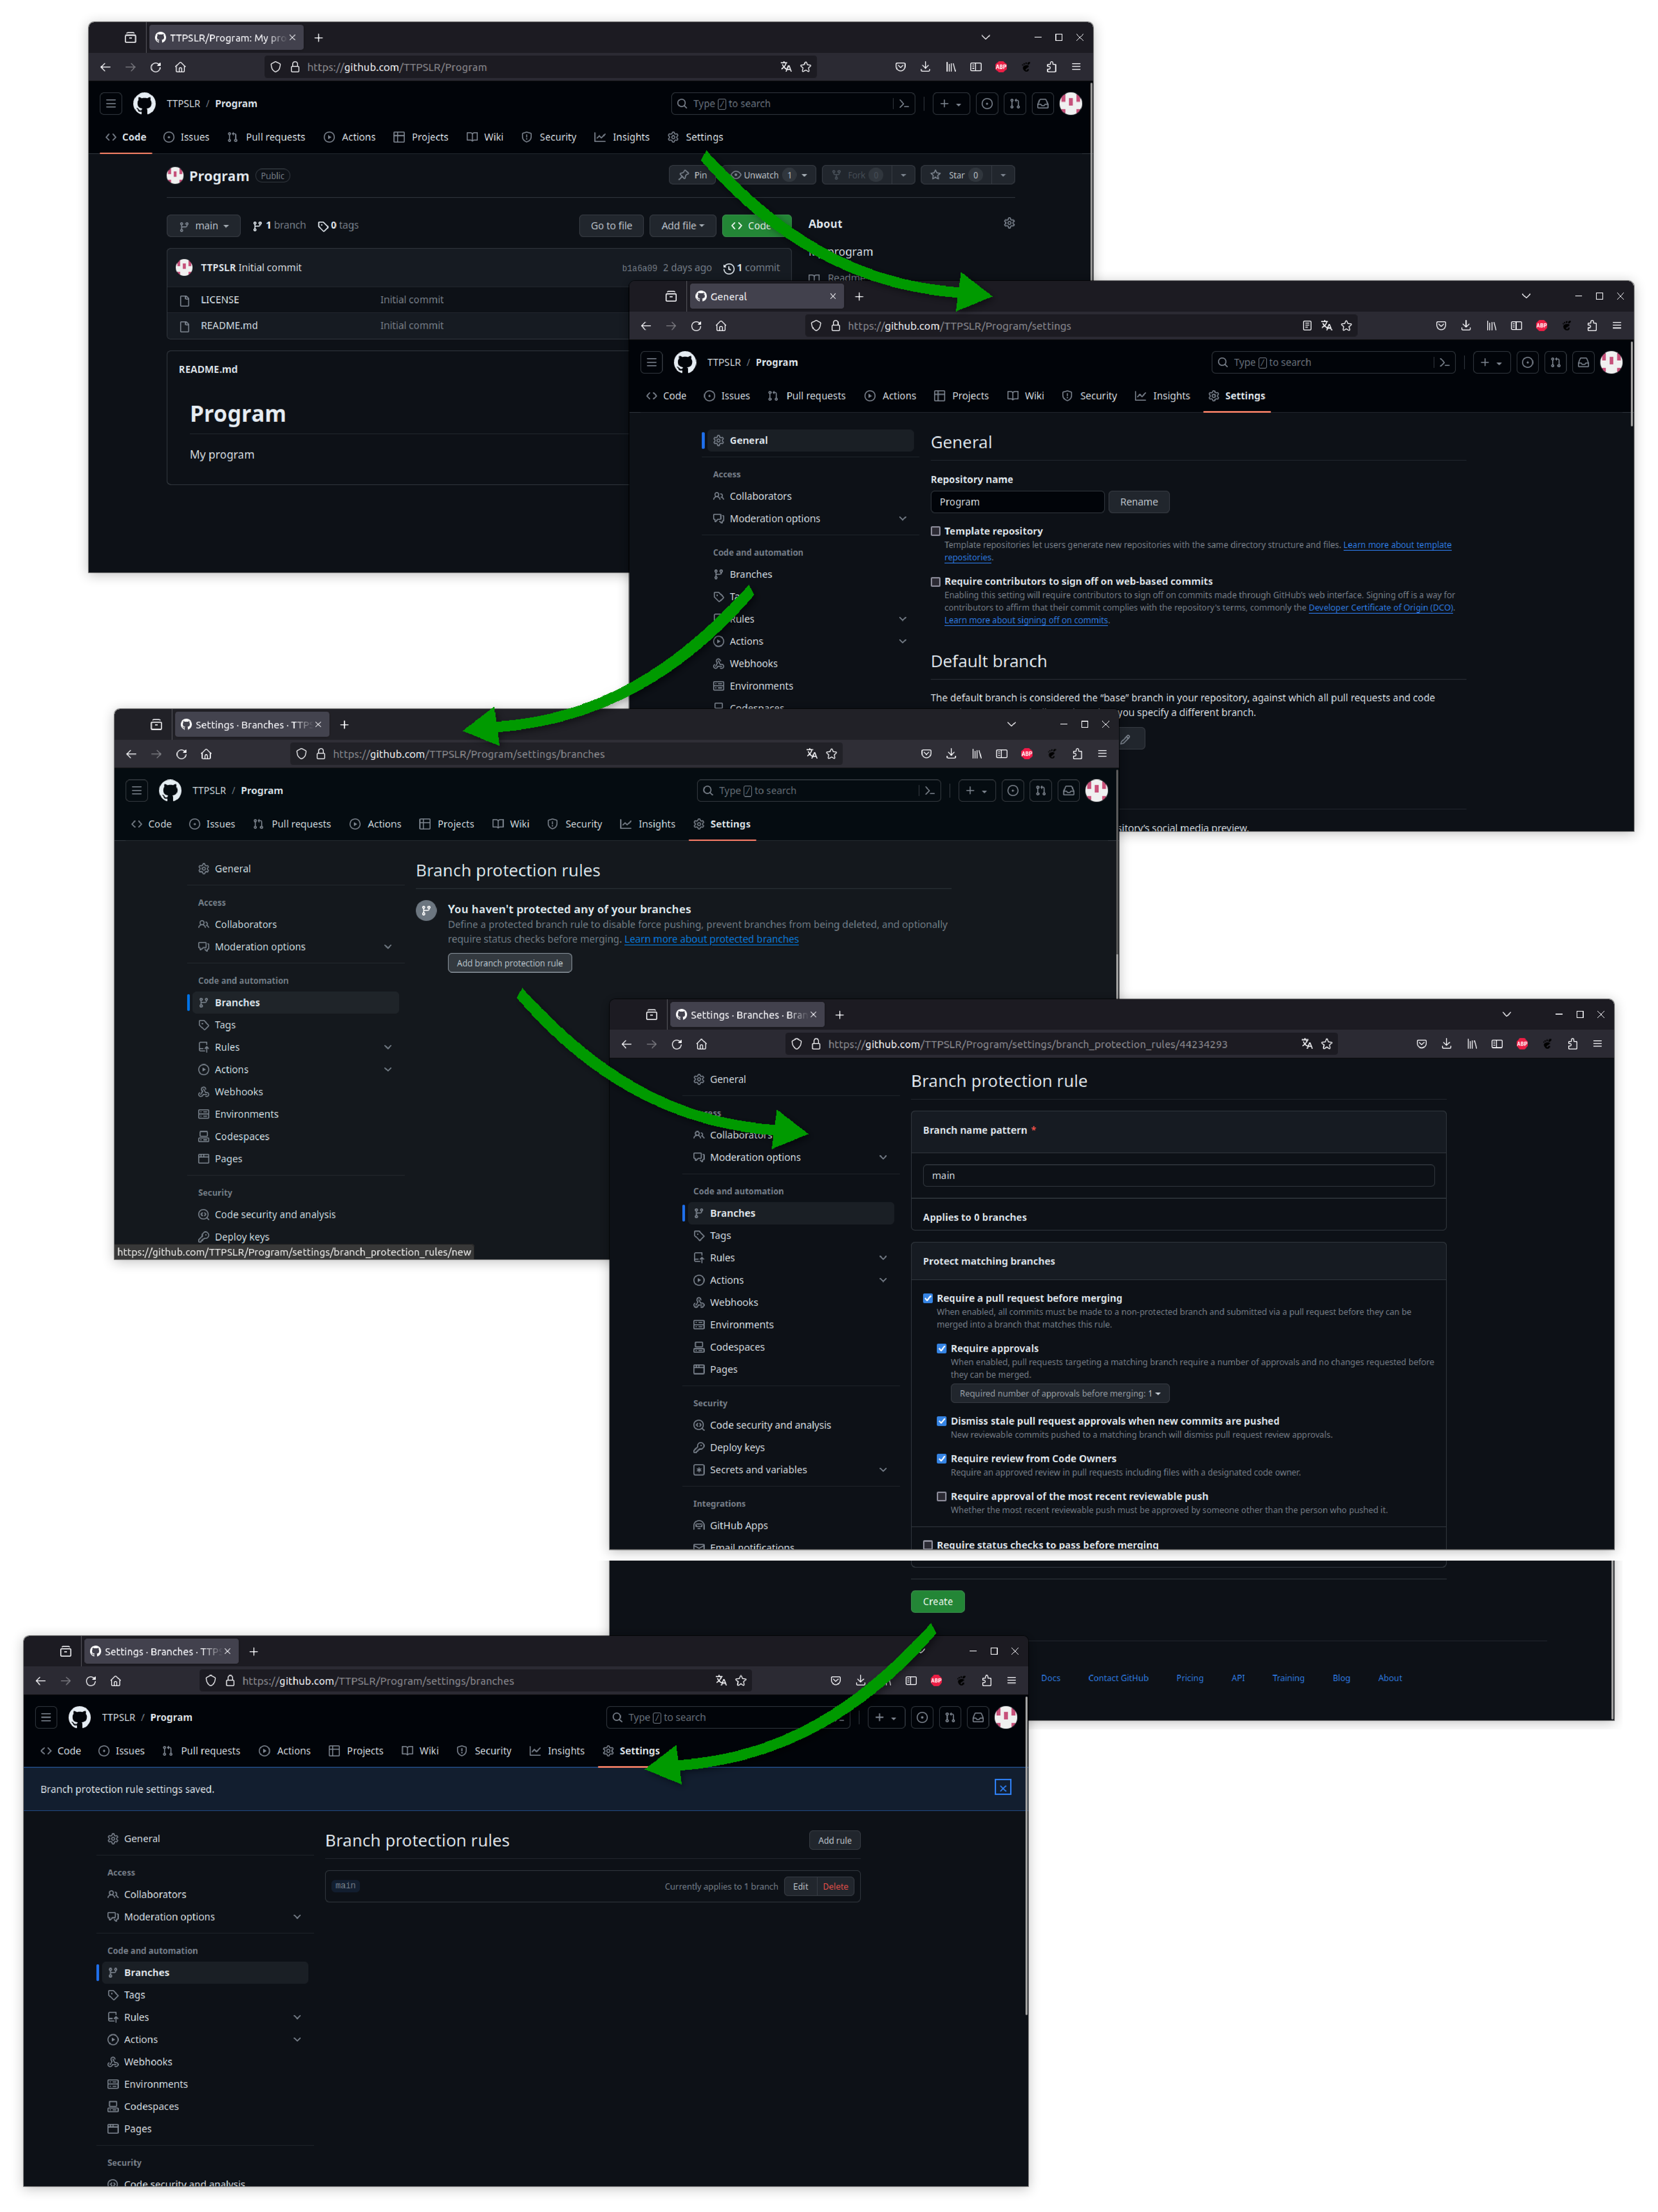
\includegraphics[width=1.0\textwidth,keepaspectratio=true,draft=\ddst]{img/hosts/github/branch.eps} 
\caption{Project branch projection on \github\label{bgithub}}
\end{figure}

\begin{figure}[!p]
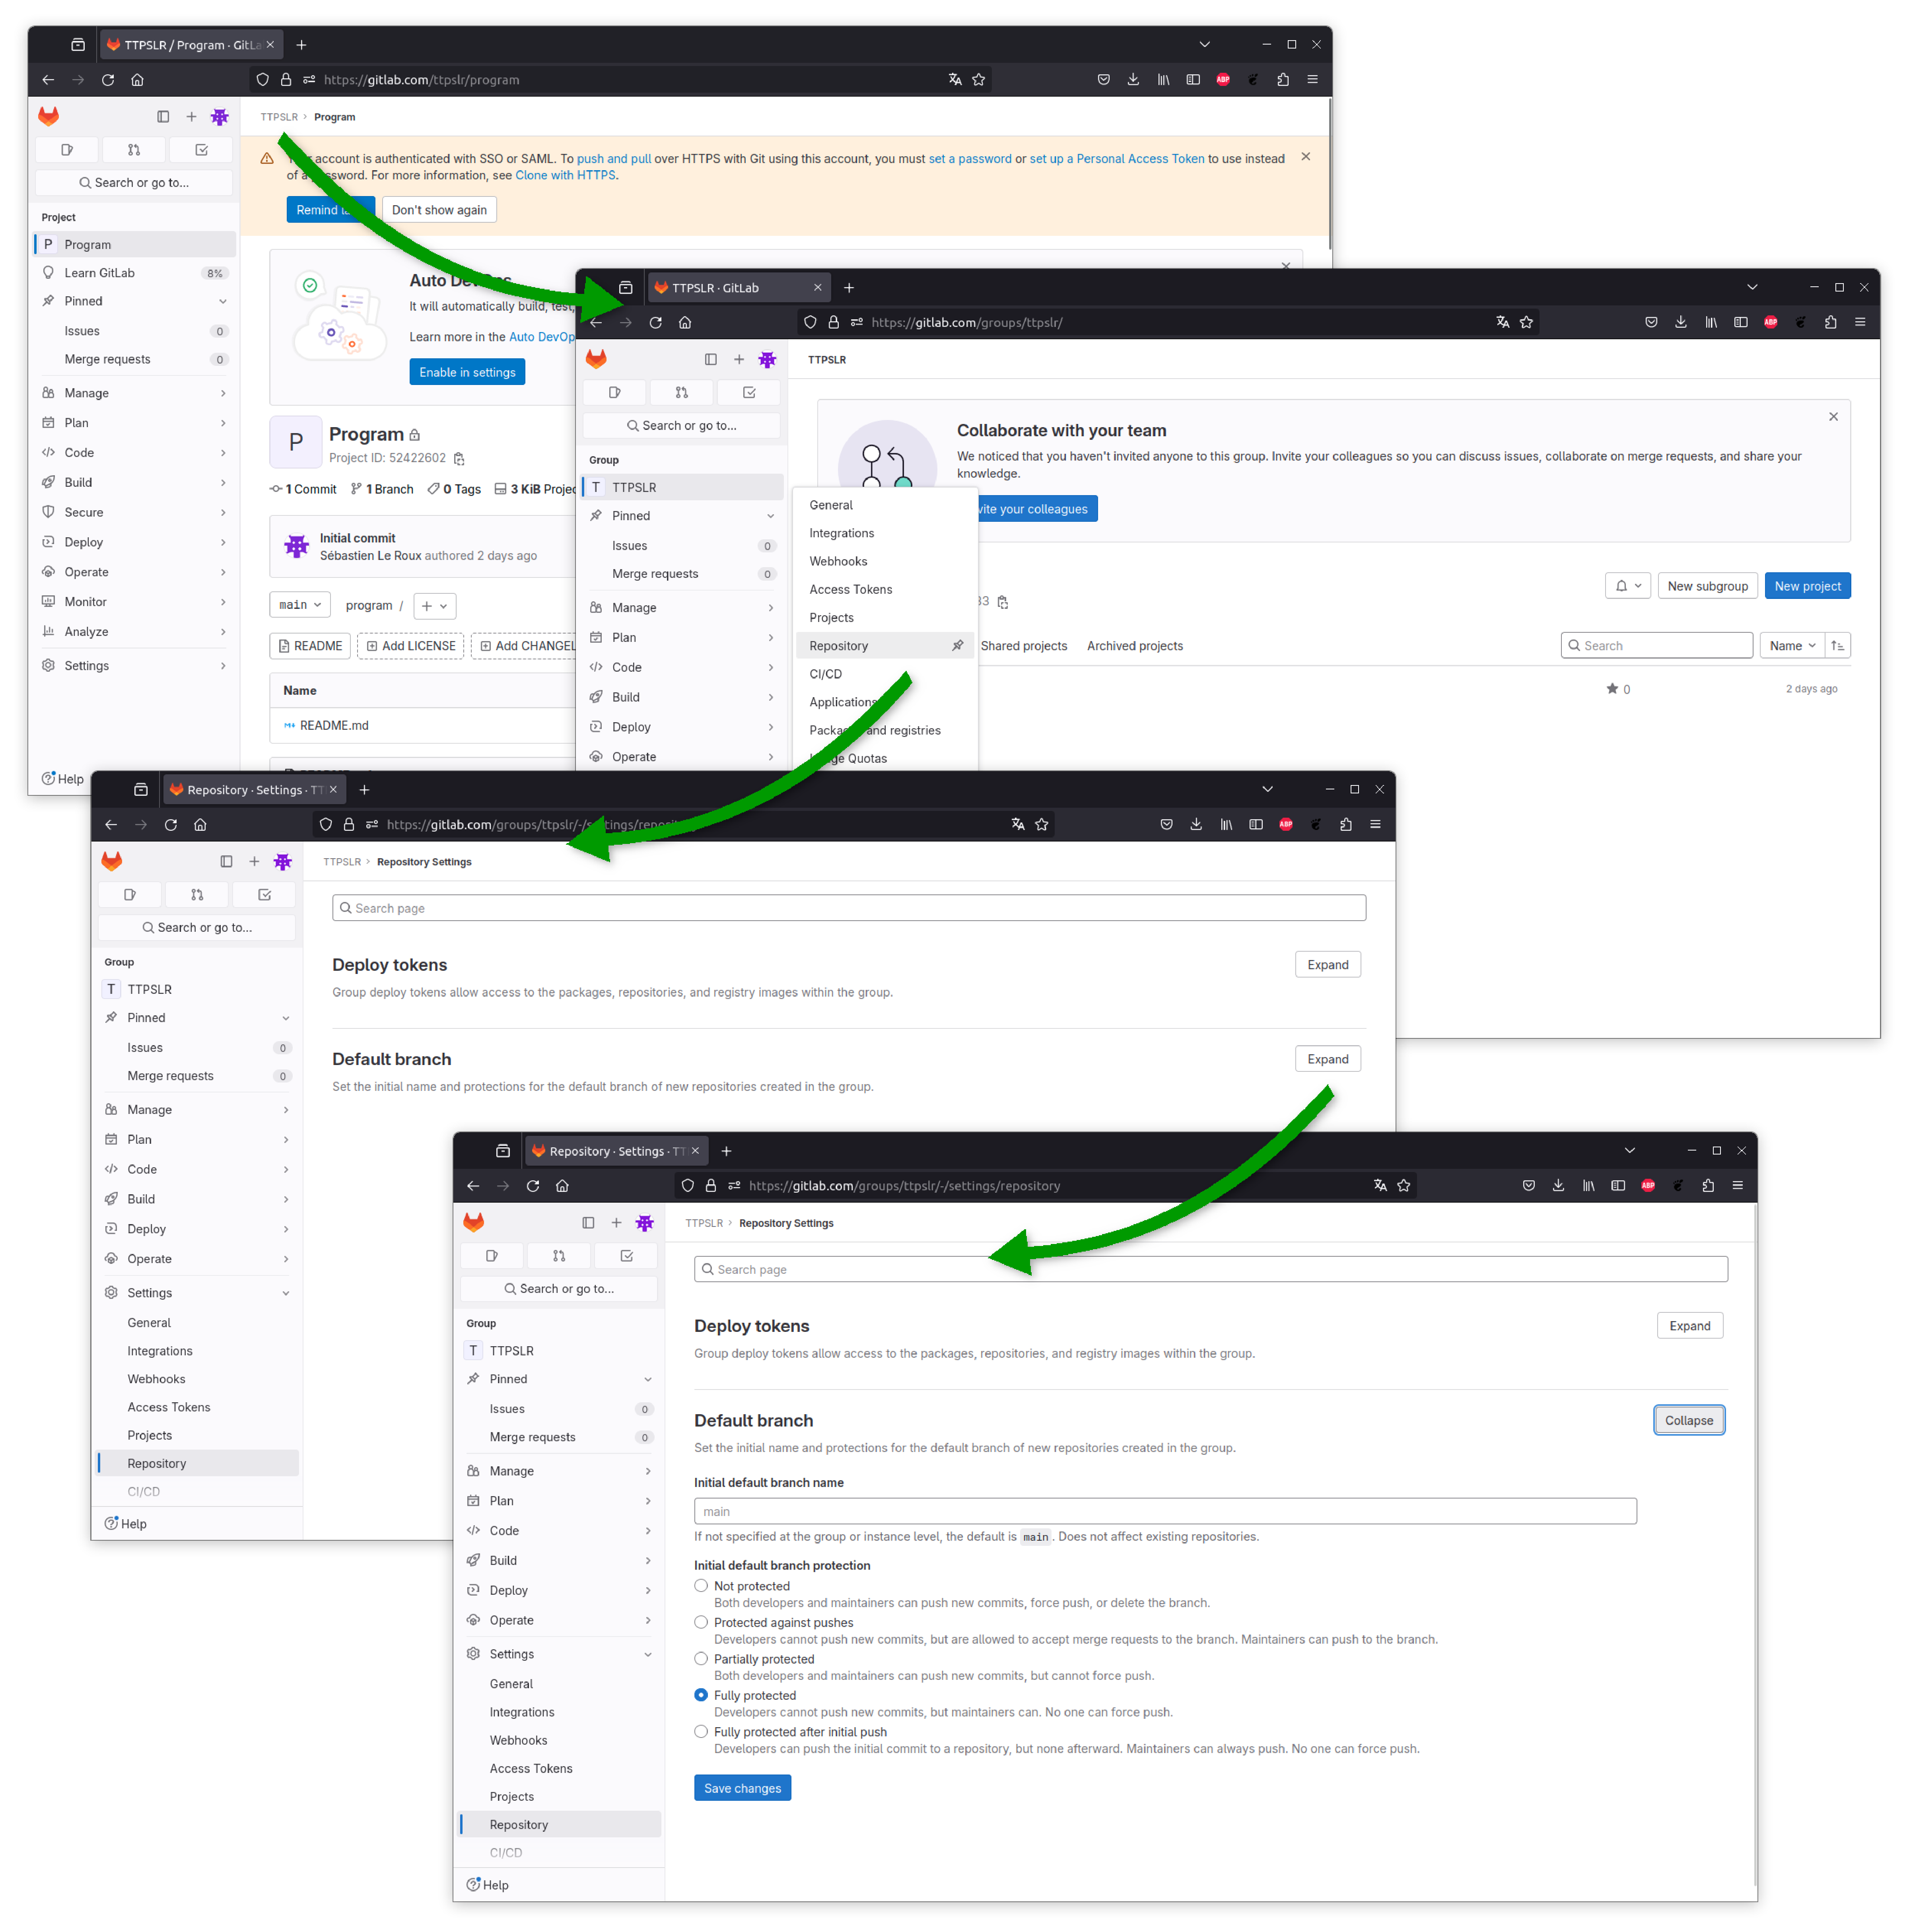
\includegraphics[width=1.0\textwidth,keepaspectratio=true,draft=\ddst]{img/hosts/gitlab/dbranch.eps} 
\caption{Default main branch projection on \gitlab\label{mbgitlab}}
\end{figure}

\begin{figure}[!p]
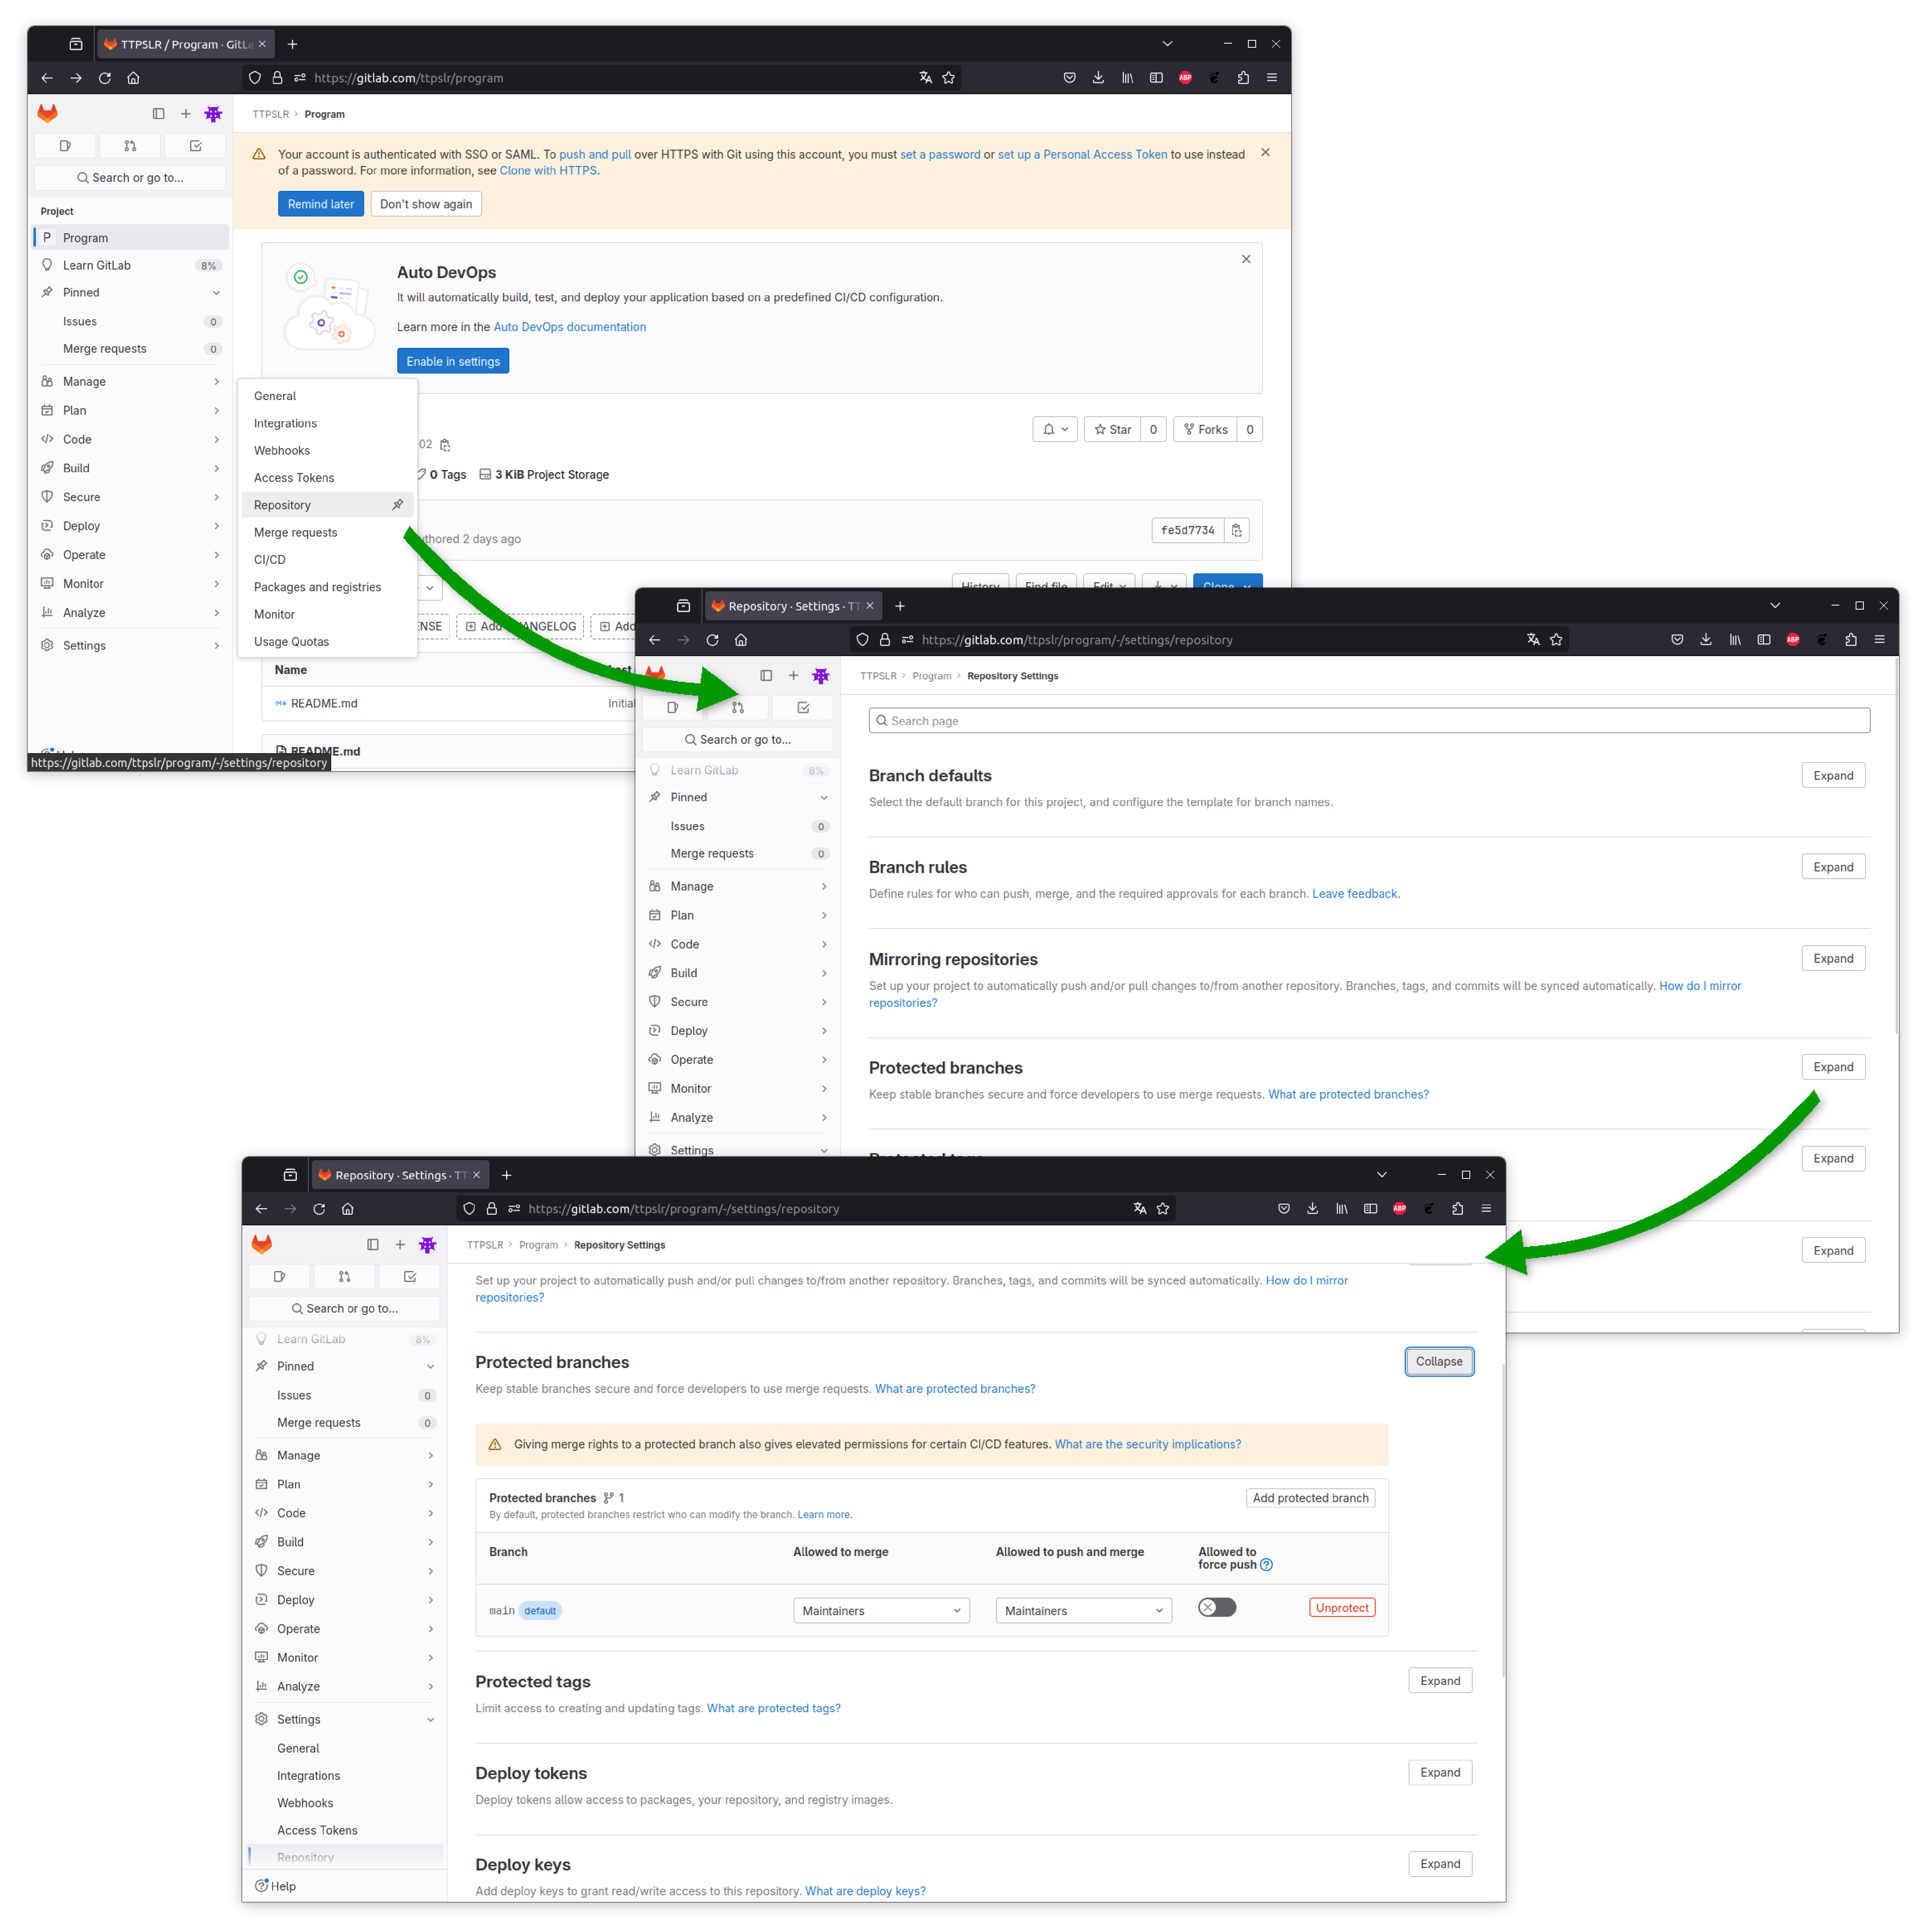
\includegraphics[width=1.0\textwidth,keepaspectratio=true,draft=\ddst]{img/hosts/gitlab/branch.eps} 
\caption{Project branch projection on \gitlab\label{bpgitlab}}
\end{figure}

\clearpage

\section{Releases and Tags}

\subsection{Tags}

On \github\ and \gitlab\ tags are images of the Git repository pointing towards archives that never change, 
like snapshots of the repository. \\
In both \github\ and \gitlab\ you can create tags whenever you think it is appropriate, 
however tags being required to produce a release, and a specific tag being associated with a specific release 
I will only focus thereafter in creating tag whenever creating release is required. 

\subsection{Releases}

On \github\ and \gitlab\ releases are deployable software versions made available for users to download. 
Releases are based on tags targeting specific points in the history of the repository. \\
To create a release: 
\begin{itemize}
\item On \github\ (see figure~\ref{rgithub}):
\begin{itemize}
\item Click on "\texttt{Create a new release}"
\item Click on "\bftt{Choose a tag}" to open the corresponding combo box:
\begin{itemize}
\item Input the new tag name, ex: "\texttt{1.0.0}" 
\item If the tag is new it is immediately proposed to create this tag
\item Click on "\bftt{Create new tag:} \bftt{1.0.0} \texttt{on publish}" \\
(or any other tag name of your choice)
\end{itemize}
\item Fill the description of the release, including release notes
\item Scroll down and click on "\texttt{Publish release}"
\end{itemize}
On \github\ releases packages have the form: "\rtt{tag}\bftt{.tar.gz}" \\
Extracting the archive on your hard drive will create a folder named: "\dgtt{repository-}\rtt{tag}"
\item On \gitlab\ (see figure~\ref{rgitlab}):
\begin{itemize}
\item On the left side menu, click on "\texttt{Deploy}" $\Longrightarrow$ "\texttt{Releases}"
\item Then click on "\texttt{Create a new release}"
\item Click on "\bftt{Tag name} \texttt{(required)}" to open the corresponding combo box:
\begin{itemize}
\item Input the new tag name, ex: "\texttt{1.0.0}" 
\item If the tag is new it is immediately proposed to create this tag
\item Click on "\texttt{Create tag} \bftt{1.0.0}" (or any other tag name of your choice)
\item Click on "\texttt{Save}"
\end{itemize}
\item Fill the description of the release, including release notes
\item Scroll down and click on "\texttt{Create release}"
\end{itemize}
On \gitlab\ releases packages have the form: "\dgtt{project}-\rtt{tag}\bftt{.tar.gz}" \\
Extracting the archive on your hard drive will create a folder named: "\dgtt{project-}\rtt{tag}"
\end{itemize}

\begin{figure}[!p]
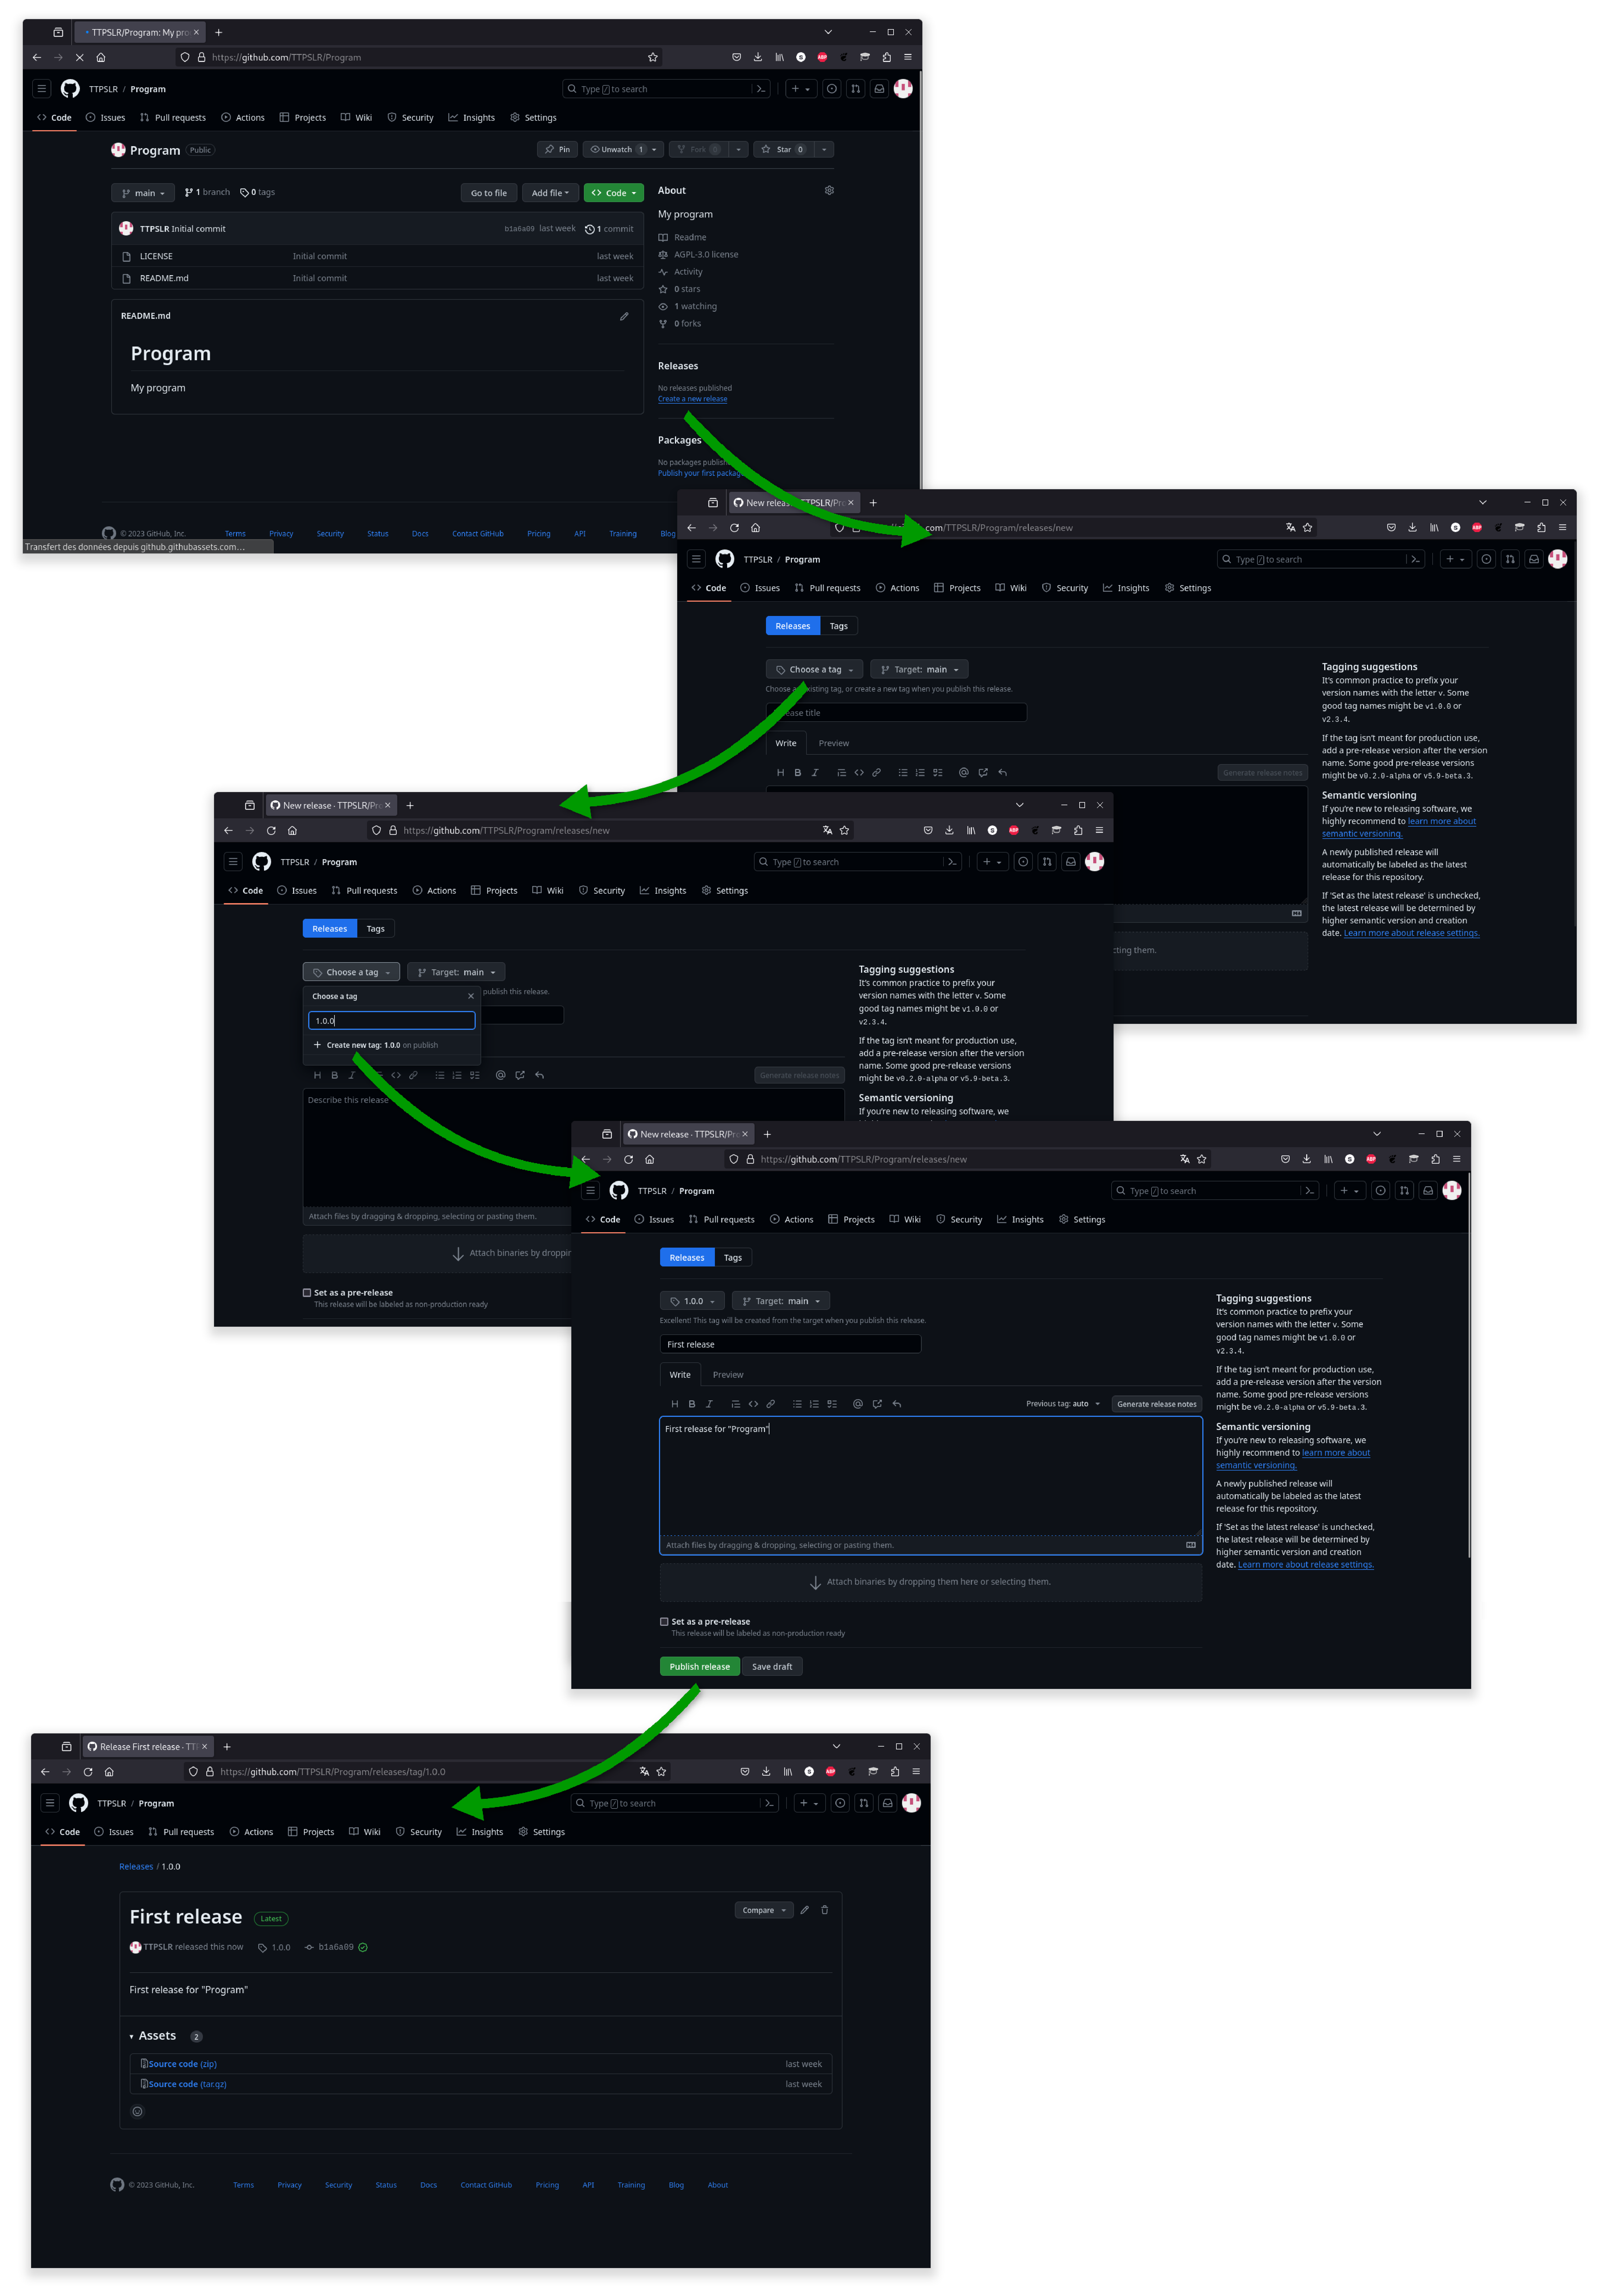
\includegraphics[width=1.0\textwidth,keepaspectratio=true,draft=\ddst]{img/hosts/github/release.eps} 
\caption{Creating a release on \github\label{rgithub}}
\end{figure}

\begin{figure}[!p]

\includegraphics[width=1.0\textwidth,keepaspectratio=true,draft=\ddst]{img/hosts/gitlab/release.eps} 
\caption{Creating a release on \gitlab\label{rgitlab}}
\end{figure}

\clearpage

\section{Using Git to manage your GitHub / GitLab project}
\label{onlinegit}

\subsection{Setting up work on you local computer} 

To start working on a remote repository using Git you can:
\begin{itemize}
\item {\bf{Clone}} the distant repository:
\begin{itemize}
\item \github:
{\footnotesize{
\begin{scriptii}
\fprompt{~/program} \bftt{git clone} git@github.com:\rtt{Author}/\btt{Program}
\end{scriptii}
}}
\item \gitlab:
{\footnotesize{
\begin{scriptii}
\fprompt{~/program} \bftt{git clone} git@gitlab.com:\rtt{Group}/\btt{Program}
\end{scriptii}
}}
\end{itemize}
\noindent Be careful \red{{\bf{NOT}}} to clone the distant repository using the "\texttt{https://git***}" instruction 
(both options being offered by \github\ and \gitlab), 
this would modify the access to the repository via the Git command line and require additional security considerations to setup 
developer access tokens, not considered in this manual. 
\item Alternatively set up manually the local folder to work remotely:
{\footnotesize{
\begin{scripti}
\fprompt{~} \bftt{mkdir} program
\fprompt{~} \bftt{cd} program
\fprompt{~/program} \bftt{git init}
\end{scripti}
}}
\begin{itemize}
\vspace{-0.5cm}
\item \github:
{\notsofoot{
\begin{scriptii}
\fprompt{~/program} \bftt{git remote} add origin git@github.com:\rtt{Author}/\btt{Program}
\end{scriptii}
}}
\\[-0.75cm]
\noindent Replace:
\begin{itemize}
\item \rtt{Name}\quad by the GitHub account that owns the repository.
\item \btt{Program}\quad by the name of the repository. \\
\end{itemize}
\item \gitlab:
{\notsofoot{
\begin{scriptii}
\fprompt{~/program} \bftt{git remote} add origin git@gitlab.com:\rtt{Group}/\btt{Program}
\end{scriptii}
}}
\\[-0.75cm]
\noindent Replace:
\begin{itemize}
\item \rtt{Group}\quad by the group Id for the GitLab account that owns the project.
\item \btt{Program}\quad by the name of the project. \\
\end{itemize}
\end{itemize}
This should be enough to get you started, providing that you check that the git user name and email are set properly (see [Sec.~\ref{gitconfig}]). \\[0.25cm]
Finally if needed setup the user information:
{\footnotesize{
\begin{scripti}
\fprompt{~} \bftt{git} \rtt{config} user.name "\abtt{Your Name}"
\fprompt{~} \bftt{git} \rtt{config} user.email \dctt{\email}
\end{scripti}
}}
\\[-0.75cm]
\noindent Replace:
\begin{itemize}
\item \rtt{Your Name}\quad by your user name. 
\item \btt{\email}\quad by your email. \\
\end{itemize}
Update the local folder with the content of the remote repository:
{\footnotesize{
\begin{scripti}
\fprompt{~/program} \bftt{git pull} origin \rtt{branch}
\end{scripti}
}}
\\[-0.75cm]
\noindent Replace:
\begin{itemize}
\item \rtt{branch}\quad by the branch of the project your are working on. 
\end{itemize} 
\end{itemize}
When this is done you can verify the link between your local folder and the on-line repository using:
\begin{script}
\fprompt{~/program} \bftt{git} remote -v
origin	git@github.com:\rtt{Author}/\btt{Program} (fetch)
origin	git@github.com:\rtt{Author}/\btt{Program} (push)
\end{script}
\\[-0.5cm]
\noindent Where:
\begin{itemize}
\item \rtt{Author}\quad is the GitHub account that owns the repository.
\item \btt{Program}\quad is the name of the repository. 
\end{itemize}

\subsection{Contributing to other project(s) and collaborative work}

If you want to work on project hosted on \github\ or \gitlab, and that you are not managing the project you intend to work on, then you need first to {\bf{fork}} this project. 
That means to create your own personnal copy of this project, independent of the original repository. \\
Afterwards to submit your modification(s) to the main repository you will need to create a dedicated branch and request to merge your branch to the main project. 
Modification(s) will be checked by a project manager, and if appropriate will be merged to the main branch of the repository. 
\newpage
\noindent To fork an exisiting project:
\begin{itemize}
\item On \github\ (see figure~\ref{fgithub}):
\begin{itemize}
\item Navigate to the \github\ project page of the repository you want to fork
\item Click on "\texttt{Fork}" to open the scrolling menu, and select "\texttt{Create a new fork}"
\item Follow the dialog to create a fork on the project in your own repository, you can select a specific branch if required, then when ready click on "\texttt{Create fork}"
\item It's done your own fork of the target project is now ready for you to work on in your own \github\ repository. 
\end{itemize}
\item On \gitlab\ (see figure~\ref{fgitlab}):
\begin{itemize}
\item Navigate to the \gitlab\ project page of the repository you want to fork
\item Click on "\texttt{Fork}"
\item Follow the dialog to create a fork on the project in your own repository, remember to specify the project URL. You can select a specific branch if required, then when ready click on "\texttt{Fork project}"
\item It's done your own fork of the target project is now ready for you to work on in your own \gitlab\ repository. 
\end{itemize}
\end{itemize}

\begin{figure}[!p]

\includegraphics[width=1.0\textwidth,keepaspectratio=true,draft=\ddst]{img/hosts/github/fork.eps} 
\caption{Creating a fork of a repository on \github\label{fgithub}}
\end{figure}
\begin{figure}[!p]
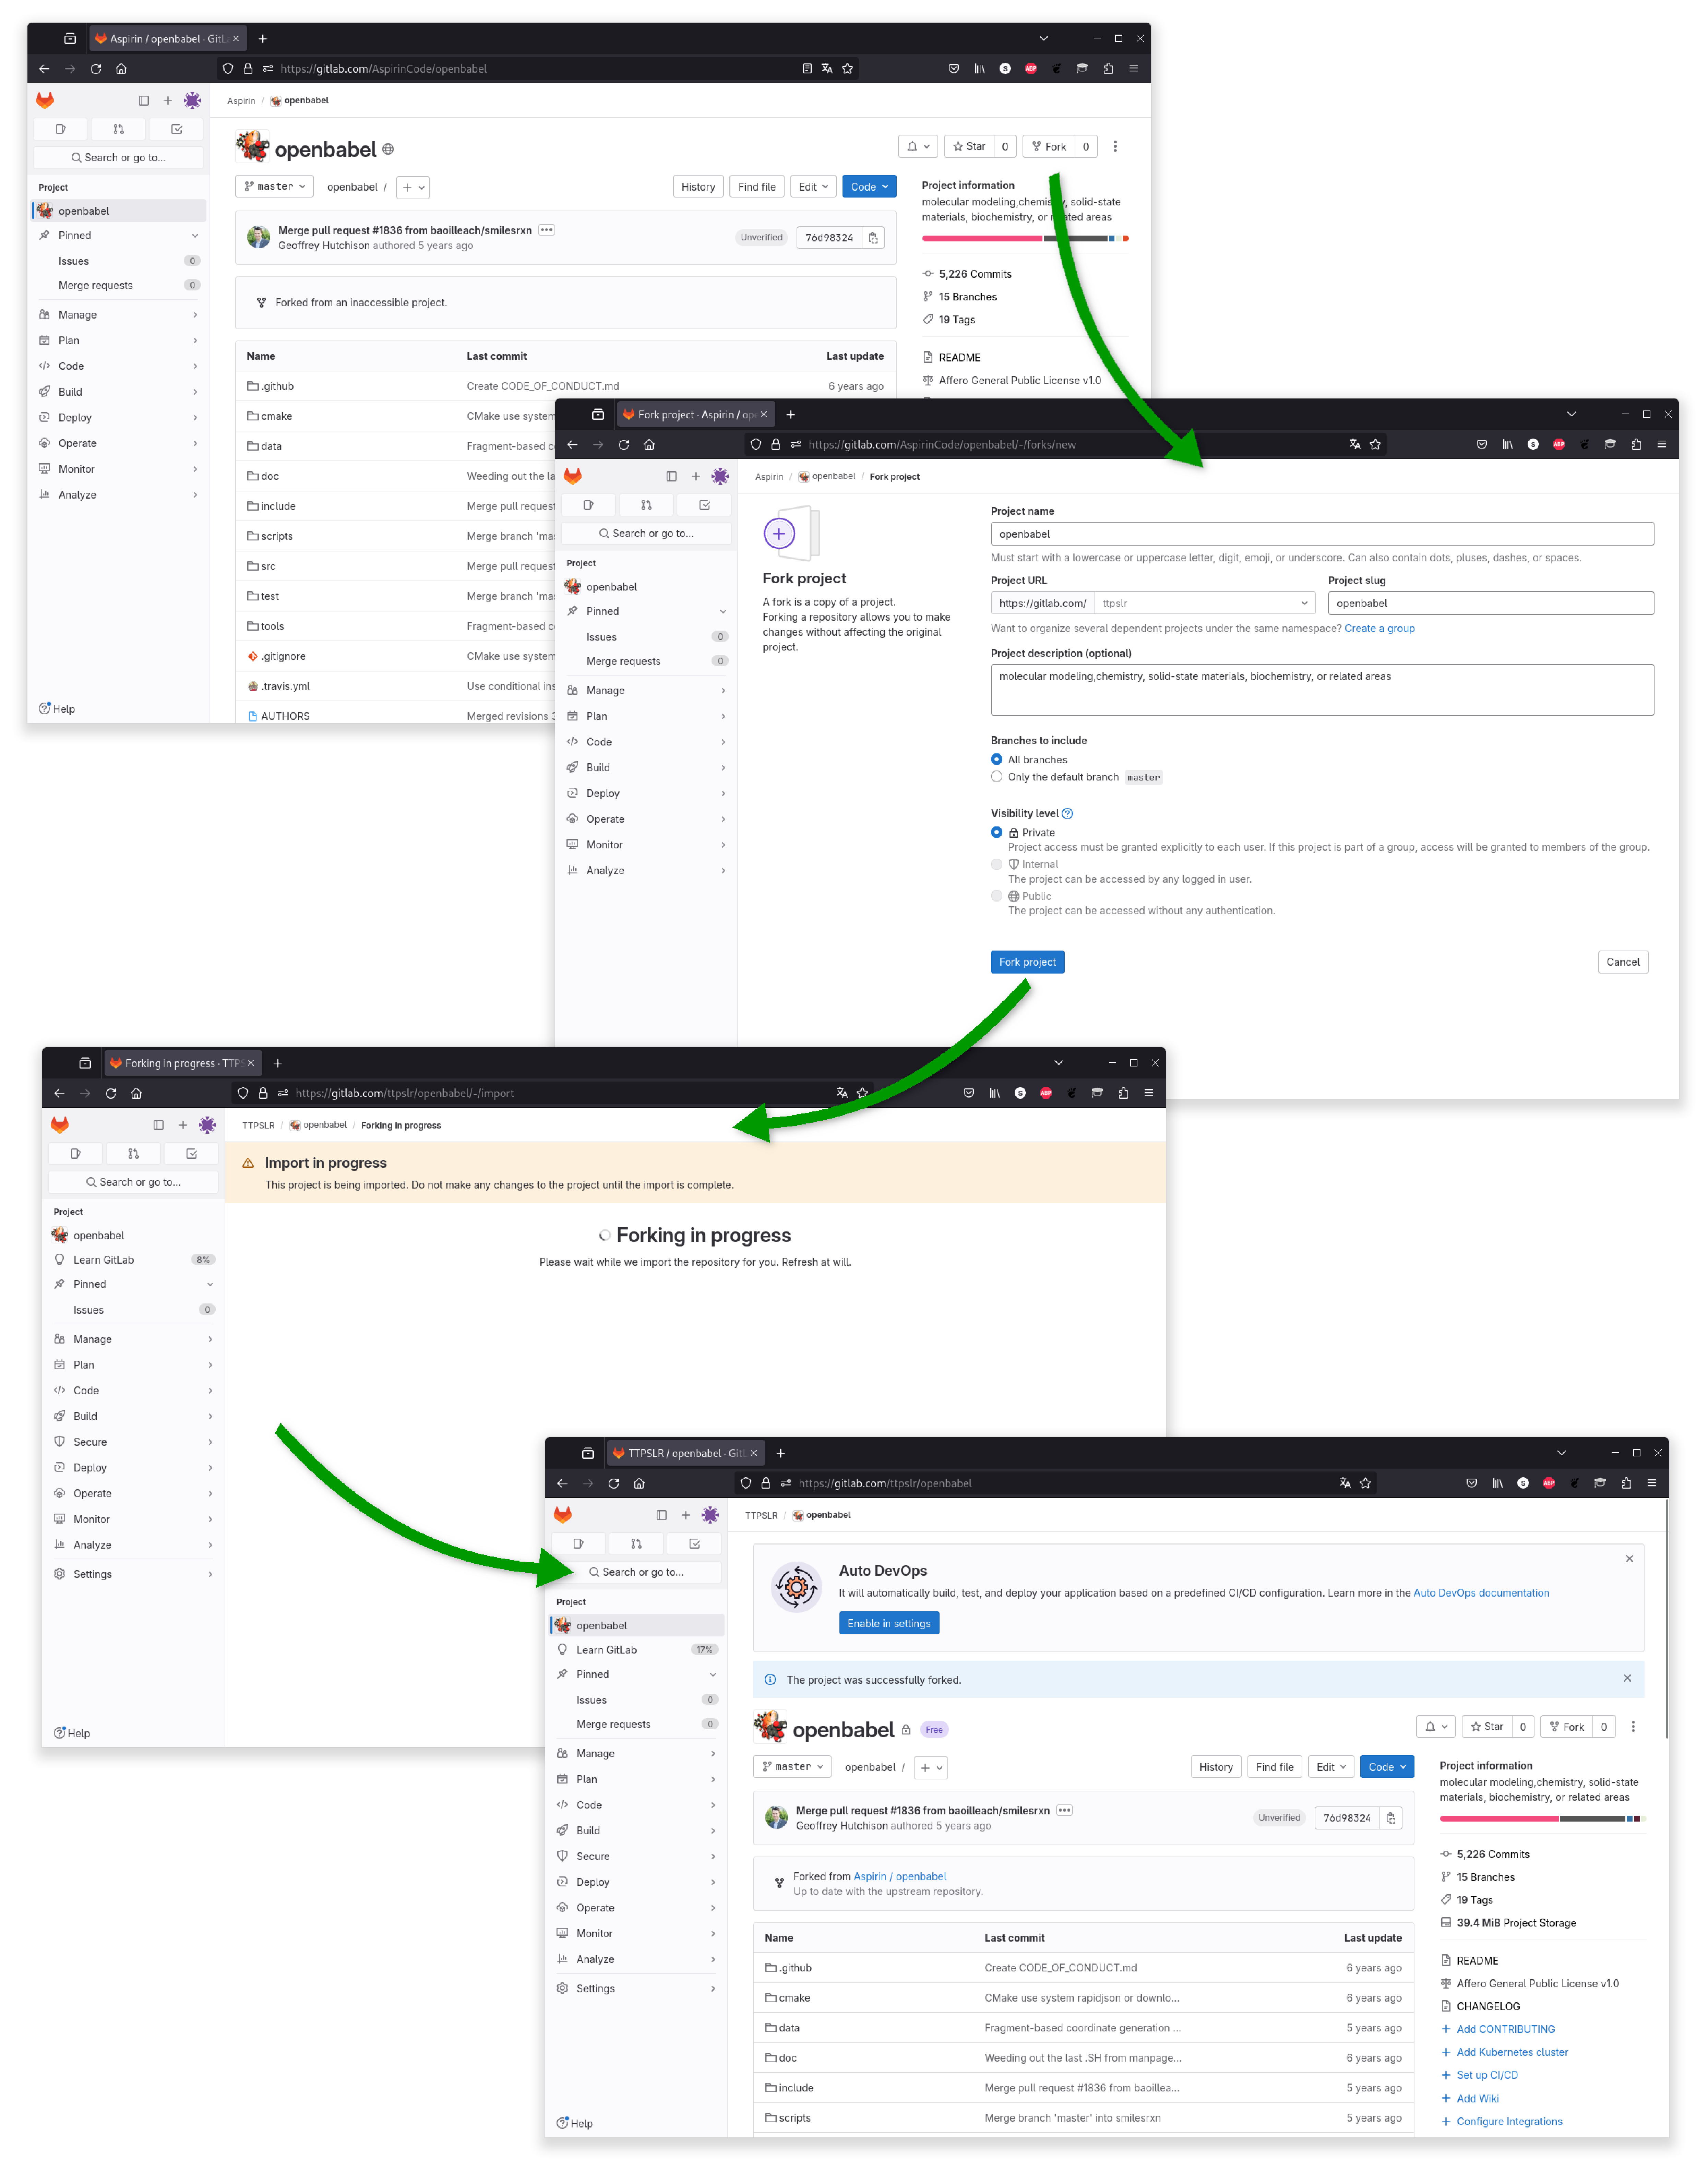
\includegraphics[width=1.0\textwidth,keepaspectratio=true,draft=\ddst]{img/hosts/gitlab/fork.eps} 
\caption{Creating a fork of a repository on \gitlab\label{fgitlab}}
\end{figure}

\newpage
\section{Project pages and documentation}

This section will illustrates how to use a \github\ / \gitlab\ repository and web pages to host a static web documentation for your project. 

\subsection{prerequisites}

It is required to install some tools to handle the publication of static webpages that will be used thereafter:
\begin{itemize}
\item Prepare the "\texttt{\textasciitilde/.bashrc}" file to install Ruby, insert the following lines:
\begin{scripti}
\fprompt{~} vi .bashrc
\comm{Install Ruby Gems to ~/gems}
\bad{export} \dctt{GEM\_HOME}\bad{=}\say{\$HOME/gems}
\bad{export} \dctt{PATH}\bad{=}\say{\$HOME/gems/bin:\$PATH}
\bad{export} \dctt{PATH}\bad{=}\say{\$HOME/.rbenv/bin:\$PATH}
\bftt{eval} \say{\$(rbenv init -)}
\bad{export} \dctt{PATH}\bad{=}\say{\$HOME/.rbenv/plugins/ruby-build/bin:\$PATH}
\end{scripti}
\item Install the Ruby dependencies (if needed)
\begin{itemize}
\item Fedora:
\vspace{-0.25cm}
{\footnotesize{
\begin{scriptii}
\textasciitilde]\$ \rtt{sudo} \bftt{dnf} install git-core gcc rust patch make bzip2 openssl-devel \textbackslash
                      libyaml-devel libffi-devel readline-devel zlib-devel \textbackslash
                      gdbm-devel ncurses-devel perl-FindBin perl-lib \textbackslash
                      perl-File-Compare
\end{scriptii}
}}
\item Debian:
\vspace{-0.25cm}
{\footnotesize{
\begin{scriptii}
\textasciitilde]\$ \rtt{sudo} \bftt{apt} install postgresql libpq-dev nodejs yarnpkg git zlib1g-dev \textbackslash
                      build-essential libssl-dev libreadline-dev libyaml-dev \textbackslash
                      libsqlite3-dev sqlite3 libxml2-dev libxslt1-dev \textbackslash
                      libcurl4-openssl-dev software-properties-common \textbackslash
                      libffi-dev
\end{scriptii}
}}
\end{itemize}
\item Install "\texttt{rbenv}":
{\footnotesize{
\begin{scripti}
\textasciitilde]\$ git clone https://github.com/rbenv/rbenv.git ~/.rbenv
\textasciitilde]\$ git clone https://github.com/rbenv/ruby-build.git ~/.rbenv/plugins/ruby-build
\textasciitilde]\$ \bftt{rbenv} \rtt{install} \dgtt{2.7.4}
\textasciitilde]\$ \bftt{rbenv} \rtt{global} \dgtt{2.7.4}
\textasciitilde]\$ \bftt{ruby} -v
\end{scripti}
}}
\\[-0.5cm]
\noindent \github\ pages are best compatible with version 2.7.x so do not install more recent release. \\
To list available stable versions:
{\footnotesize{
\begin{scripti}
\textasciitilde]\$ \bftt{rbenv} \rtt{install} \dctt{-l}
\end{scripti}
}}
\item Update "\texttt{rubygem}":
{\footnotesize{
\begin{scripti}
\textasciitilde]\$ \bftt{gem} \rtt{update} \dgtt{--system}
\end{scripti}
}}
\item Install \href{https://jekyllrb.com}{Jekyll} and the Ruby bundler:
\vspace{-0.25cm}
\begin{scripti}
\fprompt{~} \bftt{gem} \rtt{install} bundler jekyll
\end{scripti}
\end{itemize}
From this point forward the following steps are required to publish your documentation on \github\ or \gitlab\ pages:
\begin{enumerate}
\item Build the documentation of your project in \href{https://www.markdownguide.org/}{Markdown} and/or HTML language
\item Use Jekyll to convert your documentation in a static website
\item Create a repository on \github\ or \gitlab\ to host the documentation
\item Push your documentation to the web pages of the associated \github\ or \gitlab\ repository. 
\end{enumerate}

\subsection{Building the documentation in Markdown or HTML language}

It is up to you to decide how to do this, a good idea is to write your documentation in \LaTeX\ format, so that you can produce clean PDF documents. 
Then convert the \LaTeX\ files to HTML using \href{https://pandoc.org/}{pandoc}. \\
Also it allows to use your bibliography in Bib\TeX\ format and makes it easy to handle references on web pages. \\[0.25cm]
See the next section to know more about the data structure to prepare. \\[0.25cm]
Few things to take care of to use \LaTeX\ and \href{https://pandoc.org/}{pandoc} to prepare your documentation:
\begin{itemize}
\item To insert figures use PNG, or other graphic format, and not EPS as in standard \LaTeX\ documents. 
\item Be careful with the location of the images, ensure that the location, ideally in a separate and dedicated folder, 
matches the link in the HTML page. 
\item Internal references for objects not on the same HTML page will be lost when rendering the website. \\
This means that if your refer to a figure from the first chapter in the second chapter, likely on separate pages, 
you will have to correct the internal link to the proper web page. 
\item Pandoc conversion is not perfectly clean so few errors will likely require to be corrected afterwards, the best way 
to do that, is to understand the issue and to automate the correction process. \\
Among known errors to take care of:
\begin{itemize}
\item Check the table and figure captions
\item Some \LaTeX\ commands, in particular from peculiar custom packages, might not be understood by pandoc, and should be test proofed. \\[0.25cm]
For example the "\texttt{\textbackslash{Ctrl}}" command from the "\texttt{keystroke}" package (to render a drawing of the keyboard control key) 
cannot be processed by pandoc and should be replace by a command having the proper effect in HTML format, 
in this case "\texttt{\textbackslash{newcommand}\{\textbackslash{Ctrl}\}\{<kbd>Ctrl<\/kbd>\}}"
\end{itemize}
\item Finally to render \LaTeX\ math and equations in your HTML page insert the following code at the top of the HTML page:
\begin{itemize}
\item To render math using \href{https://www.mathjax.org/}{mathjax} use:
{\notsotiny{
\begin{scriptii}
\dbtt{<script} \abtt{src=}\red{"https://polyfill.io/v3/polyfill.min.js?features=es6"}\dbtt{></script>}
\dbtt{<script} \abtt{id=}\red{"MathJax-script" async src="https://cdn.jsdelivr.net/npm/mathjax@3.0.1/es5/tex-mml-chtml.js"}\dbtt{></script>}
\end{scriptii}
}}
\item To render math using \href{https://katex.org/}{katex} use:
{\notsotiny{
\begin{scriptii}
\dbtt{<script} \abtt{src=}\red{"https://cdnjs.cloudflare.com/ajax/libs/KaTeX/0.11.1/katex.min.js"}\dbtt{></script>}
\dbtt{<script>}document.addEventListener("DOMContentLoaded", function () {
   var mathElements = document.getElementsByClassName("math");
   var macros = [];
   for (var i = 0; i < mathElements.length; i++) {
      var texText = mathElements[i].firstChild;
      if (mathElements[i].tagName == "SPAN") {
       katex.render(texText.data, mathElements[i], {
        displayMode: mathElements[i].classList.contains({\textquotesingle}display{\textquotesingle}),
        throwOnError: false,
        macros: macros,
        fleqn: false
        });
      }}});
\dbtt{</script>}
\dbtt{<link} \abtt{rel=}\red{"stylesheet" href="https://cdnjs.cloudflare.com/ajax/libs/KaTeX/0.11.1/katex.min.css"} \dbtt{/>}
\dbtt{<!--}\abtt{[if lt IE 9]}\dbtt{>}
  \dbtt{<script} \abtt{src=}\red{"//cdnjs.cloudflare.com/ajax/libs/html5shiv/3.7.3/html5shiv-printshiv.min.js"}\dbtt{></script>}
\dbtt{<!}\abtt{[endif]}\dbtt{-->}
\end{scriptii}
}}
\end{itemize}
\end{itemize}
\vspace{-0.25cm}
Overall this method requires some additional work to properly convert the documents to a clean simple combination of Markdown and HTML structure, 
but once this work is automated you will only write your documentation using \LaTeX\ and then, in a single command, 
convert it and publish it to \github\ or \gitlab\ pages. 

\subsection{Using Jekyll to build a static website}

\href{https://jekyllrb.com}{Jekyll} is a simple static site generator. \\
Think of it like a file-based CMS, without all the complexity. Jekyll takes your content, renders Markdown and Liquid templates, 
and creates a complete, static website ready to be served by any web server. \\
Jekyll is the engine behind GitHub Pages, which you can use to host sites right from your GitHub repositories. \\[0.25cm]
Jekyll expects a document structure with Markdown files, but can also handles HTML files as includes files. 
In the following I will illustrate the document structure required by Jekyll to build a static web site: 
\begin{itemize}
\item For \LaTeX\ converted to HTML documentation
\item Using bibliography references in the \href{https://www.bibtex.org/}{Bib\TeX} format
\end{itemize}
Example repository to create the documentation: 
{\footnotesize{ 
\begin{script}
\fprompt{~/Program-doc} \bftt{ls}
\btt{\_bibliography}  \btt{chap-1}  \btt{intro}  \_config.yml  Gemfile  \btt{\_includes}  README.md
\end{script}
}}
\noindent With:
\begin{itemize}
\item Files:
\begin{itemize}
\item The home page of your documentation website: "\texttt{README.md}"
\item The list of Ruby extensions required to build your website: "\texttt{Gemfile}"
{\scriptsize{
\begin{scriptii}
\fprompt{~/Program-doc} \bftt{vi} Gemfile
source "\magenta{https://rubygems.org}"

\var{gem} {\textquotesingle}\magenta{jekyll-rtd-theme}{\textquotesingle}
\var{gem} {\textquotesingle}\magenta{github-pages}{\textquotesingle}, \magenta{group}: :\magenta{jekyll\_plugins}
\var{gem} {\textquotesingle}\magenta{jekyll-scholar}{\textquotesingle}, \magenta{group}: :\magenta{jekyll\_plugins}
group :\magenta{jekyll\_plugins} \bbtt{do}
  \var{gem} "\magenta{jekyll}", "\magenta{~> 3.9.0}"
  \var{gem} "\magenta{jekyll-feed}", "\magenta{~> 0.12}"
  \var{gem} "\magenta{jekyll-paginate}"
  \var{gem} "\magenta{jekyll-seo-tag}"
  \var{gem} "\magenta{jekyll-sitemap}"
  \var{gem} "\magenta{jekyll-archives}"
  \var{gem} "\magenta{jekyll-redirect-from}"
\bbtt{end}

\comm{Windows and JRuby does not include zoneinfo files,}
\comm{so bundle the tzinfo-data gem and associated library.}
platforms \magenta{:mingw}, \magenta{:x64\_mingw}, \magenta{:mswin}, \magenta{:jruby} \bbtt{do}
  \var{gem} "\magenta{tzinfo}", "\magenta{~> 1.2}"
  \var{gem} "\magenta{tzinfo-data}"
\bbtt{end}

\comm{ Performance-booster for watching directories on Windows}
\var{gem} "\magenta{wdm}", "\magenta{~> 0.1.1}", \magenta{:platforms} => [\magenta{:mingw}, \magenta{:x64\_mingw}, \magenta{:mswin}]
\end{scriptii}
}}
\item The Jekkyl configuration file to build the website: "\texttt{\_config.yml}"\\[-0.5cm] 
{\scriptsize{
\begin{scriptii}
\fprompt{~/Program-doc} \bftt{vi} \_config.yml
\var{title:} Program's documentation
\var{baseurl:} \magenta{"/Program-doc"}
\var{url:} \magenta{""}
\comm{GitHub or GtiLab repository:}
\var{repository:} TTPSLR/Program-doc
\var{lang:} en
\var{description:} This site presents the documentation for "Program"
\var{markdown:} kramdown
\var{highlighter:} rouge
\var{gist:}
  \var{noscript:} \magenta{false}
\var{kramdown:}
  \var{math\_engine:} mathjax
  \var{syntax\_highlighter:} rouge
\var{markdown\_extensions:}
  - \var{toc:}
    \var{permalink:} \magenta{"#"}
\comm{Define the depth of the menu}
    \var{baselevel:} 2
\var{banner:} \magenta{"/assets/img/banner.png"}
\var{favicon:} \magenta{"/assets/img/favicon.ico"}
\var{remote\_theme:} rundocs/jekyll-rtd-theme
\var{readme\_index:}
  \var{with\_frontmatter:} \magenta{true}

\var{plugins:}
  - jekyll-coffeescript
  - jekyll-default-layout
  - jekyll-gist
  - jekyll-github-metadata
  - jekyll-optional-front-matter
  - jekyll-paginate
  - jekyll-readme-index
  - jekyll-titles-from-headings
  - jekyll-relative-links
  - jekyll-scholar
  - jekyll-feed
  - jekyll-paginate
  - jekyll-seo-tag
  - jekyll-sitemap
  - jekyll-archives
  - jekyll-redirect-from
  - jekyll-remote-theme

\var{scholar:}
  \var{locale:} en
  \var{source:} ./\_bibliography
  \var{style:} \_bibliography/my-ieee.cls
  \var{bibliography:} references.bib
  \var{bibliography\_template:} \magenta{""}
  \var{replace\_strings:} \magenta{true}
  \var{join\_strings:}    \magenta{true}
  \var{use\_raw\_bibtex\_entry:} \magenta{false}
  \var{details\_dir:}    bibliography
  \var{details\_layout:} bibtex.html
  \var{details\_link:}   Details
\comm{Ensure that details are not printed twice}
  \var{query:} \magenta{"@*"}

\var{exclude:}
  - CNAME
  - Gemfile
  - Gemfile.lock
\end{scriptii}
}}
\end{itemize}
\item Directories:
\begin{itemize}
\item Each chapter or section in a separate directory, in this case "\btt{intro}" and "\btt{chap-1}":
\vspace{-0.25cm}
{\footnotesize{
\begin{scriptii}
\fprompt{~/program-doc} \bftt{ls} intro
README.md

\fprompt{~/program-doc} \lsr\ chap-1

chap-1:
README.md  \btt{section-1}  \btt{section-2}

chap-1/section-1:
README.md

chap-1/section-2:
README.md
\end{scriptii}
}}\\[-0.5cm]
\noindent Including sub-directories for chapter sections if required. \\
Note that each directory contains a single "\texttt{README.md}" file, dedicated to a single page of your site. \\[0.25cm]
\item Include files in the "\btt{\_includes}" directory:
{\footnotesize{
\begin{scriptii}
\fprompt{~/program-doc} \lsr\ \_includes
.:
\btt{intro}  \btt{chap-1}

./intro:
intro.html

./chap-1:
chap-1.html  \btt{section-1}  \btt{section-2}

./chap-1/section-1:
section-1.html

./chap-1/section-2:
section-2.html
\fprompt{~/program-doc}
\end{scriptii}
}} \\[-0.5cm]
\noindent including sub-directories for appendix chapters and sections if required. 
\newpage
\item The bibliography in the "\btt{\_bibliography}" directory:
{\footnotesize{
\begin{scriptii}
\fprompt{~/program-doc} \bftt{ls} \_bibliography
my-ieee.cls  references.bib
\end{scriptii}
}}
With:
\begin{itemize}
\item The "\texttt{*.ieee.cls}" file contains the bibliography style to apply
\item The "\texttt{*.bib}" file contains references in \href{https://www.bibtex.org/}{Bib\TeX} format \\
When you convert \LaTeX\ to HTML the keywords for the bibliography remain in the HTML document.
\end{itemize}
\end{itemize}
\end{itemize}
The "\texttt{README.md}" files, in Markdown format, follow the structure: 
{\footnotesize{
\begin{script}
\fprompt{~/program-doc} \bftt{vi} chap-1/README.md
\mdcom{This is a HTML comment in Markdown}
\mdcom{It will show up in the converted HTML document}

---
\mdcom{Position of this file in the website menu.}
\mdcom{To be compared will all other README.md file(s) at the same level,}
\mdcom{in this case all "~/program-doc/*/README.md" files}
sort: 2
\mdcom{Creation date:}
date: 2023-11-26
\mdcom{Math formula on this pages ?}
\mdcom{This is used to enable math javascript:}
maths: 1
---

\mdcom{# is the Markdown command for a heading}
\mdcom{Therefore the next line is the title of the chapter}
\magenta{# How to use "Program"}
\mdcom{Note if you do that you need to remove the heading line}
\mdcom{from the included HTML file bellow:}

\mdcom{Jekyll instruction to read an include file,}
\mdcom{and search for corresponding file(s) in the "\_include" folder}
\{\% include chap-1/chap-1.html \%\}

\mdcom{Jekyll instruction to process all sub-directories, if any:}
\{\% include list.liquid all=true \%\}

\mdcom{Jekyll instruction to add a bibliography section on this page:}
\{\% bibliography --cited \%\}
\mdcom{Then Jekyll search the "\_bibliography" folder to insert references}
\end{script}
}}
\clearpage
\noindent Jekyll will search for all "\texttt{README.md}" files in the directory tree, starting from the top directory. 
and build the website according to the "\texttt{sort}" instructions, in this example:
\begin{itemize}
\item Top level, homepage: "\texttt{README.md}"
\begin{itemize}
\item First level: \\
\begin{itemize}
\item In "\texttt{intro\textbackslash README.md}"  \,\,\ \quad$\Longrightarrow$\quad "\texttt{sort: }\rtt{1}"\\
\item In "\texttt{chap-\rtt{1}\textbackslash README.md}" \quad$\Longrightarrow$\quad "\texttt{sort: }\rtt{2}"\\
\item[$-$] Second level (chapter sections): \\
\begin{itemize}
\item In "\texttt{chap-1\textbackslash section-\rtt{1}\textbackslash README.md}" \quad$\Longrightarrow$\quad "\texttt{sort: }\rtt{1}"\\
\item In "\texttt{chap-1\textbackslash section-\rtt{2}\textbackslash README.md}" \quad$\Longrightarrow$\quad "\texttt{sort: }\rtt{2}"\\
\end{itemize}
\end{itemize}
\end{itemize}
\end{itemize}
Jekyll will create a HTML page for each "\texttt{README.md}" file found in the directory tree. \\
For your documentation to be easy to browse and read take time to organize it properly and split the pages accordingly. \\
The directories "\texttt{\_includes}" and "\texttt{\_bibliography}" are ignored by Jekyll when searching for "\texttt{README.md}" files, 
however their content is used to produce the website. \\[0.25cm]
To install the packages required by the "\texttt{Gemfile}" to build your site use:
\begin{script}
\fprompt{~/Program-doc} \bftt{bundle} \rtt{install}
\end{script}\\[-0.75cm]
\noindent Then to build the site use:
\begin{script}
\fprompt{~/Program-doc} \bftt{bundle} \rtt{exec} \dgtt{jekyll} build
\end{script}\\[-0.75cm]
\noindent You will see that this command creates a new directory name "\texttt{\_site}" that contains your website. 
\begin{script}
\fprompt{~/Program-doc} ls \_site

\end{script}\\[-0.75cm]
\noindent You can give a try to this website on your computer using: 
\begin{script}
\fprompt{~/Program-doc} \bftt{bundle} \rtt{exec} \dgtt{jekyll} serve
\end{script}\\[-0.75cm]
\noindent And simply follow the instructions.
\newpage

\subsection{Hosting the website on GitHub}

To use \github\ to host your documentation: 
\begin{itemize}
\item Create a dedicated repository, in the following example: "\texttt{TTPSLR/Program-doc}"
\item After properly configuring the connection to the remote repository, upload the contents of the "\texttt{\textasciitilde/Program-doc}" but the folder "\texttt{\_site}" to the main branch, separate branches allows to keep track of both the source material and the final content of the website:
\begin{scriptii}
\fprompt{~/Program-doc} \bftt{mv} \_site ../
\fprompt{~/Program-doc} \bftt{git} \rtt{checkout} \btt{-b} Main
\fprompt{~/Program-doc} \bftt{git} \rtt{add} .
\fprompt{~/Program-doc} \bftt{git} \rtt{commit} \btt{-m} "To build the doc"
\fprompt{~/Program-doc} \bftt{git} \rtt{push} \btt{origin} Main
\end{scriptii}
\item After properly configuring the connection to the remote repository, upload the contents of the "\texttt{\_site}" to the \github\ pages, the "\texttt{gh-pages}" branch:
\begin{scripti}
\fprompt{~/\_site} \bftt{git} \rtt{checkout} \btt{-b} gh-pages
\fprompt{~/\_site} \bftt{git} \rtt{add} .
\fprompt{~/\_site} \bftt{git} \rtt{commit} \btt{-m} "Documentation"
\fprompt{~/\_site} \bftt{git} \rtt{push} \btt{origin} gh-pages
\end{scripti}
\end{itemize}
After a short while the result is updated, and as is illustrated on figure~\ref{dgithub}, the website is alive. \\
Open the "\texttt{Pages}" tab in the "\texttt{Settings}" menu, to find out the web address of your site. \\
In this example: \href{https://ttpslr.github.io/Program-doc}{https://ttpslr.github.io/Program-doc} \\[0.25cm]
The \github\ pages address have the form:\quad https://\rtt{Author}.github.io/\btt{Program}

\begin{figure}[!p]
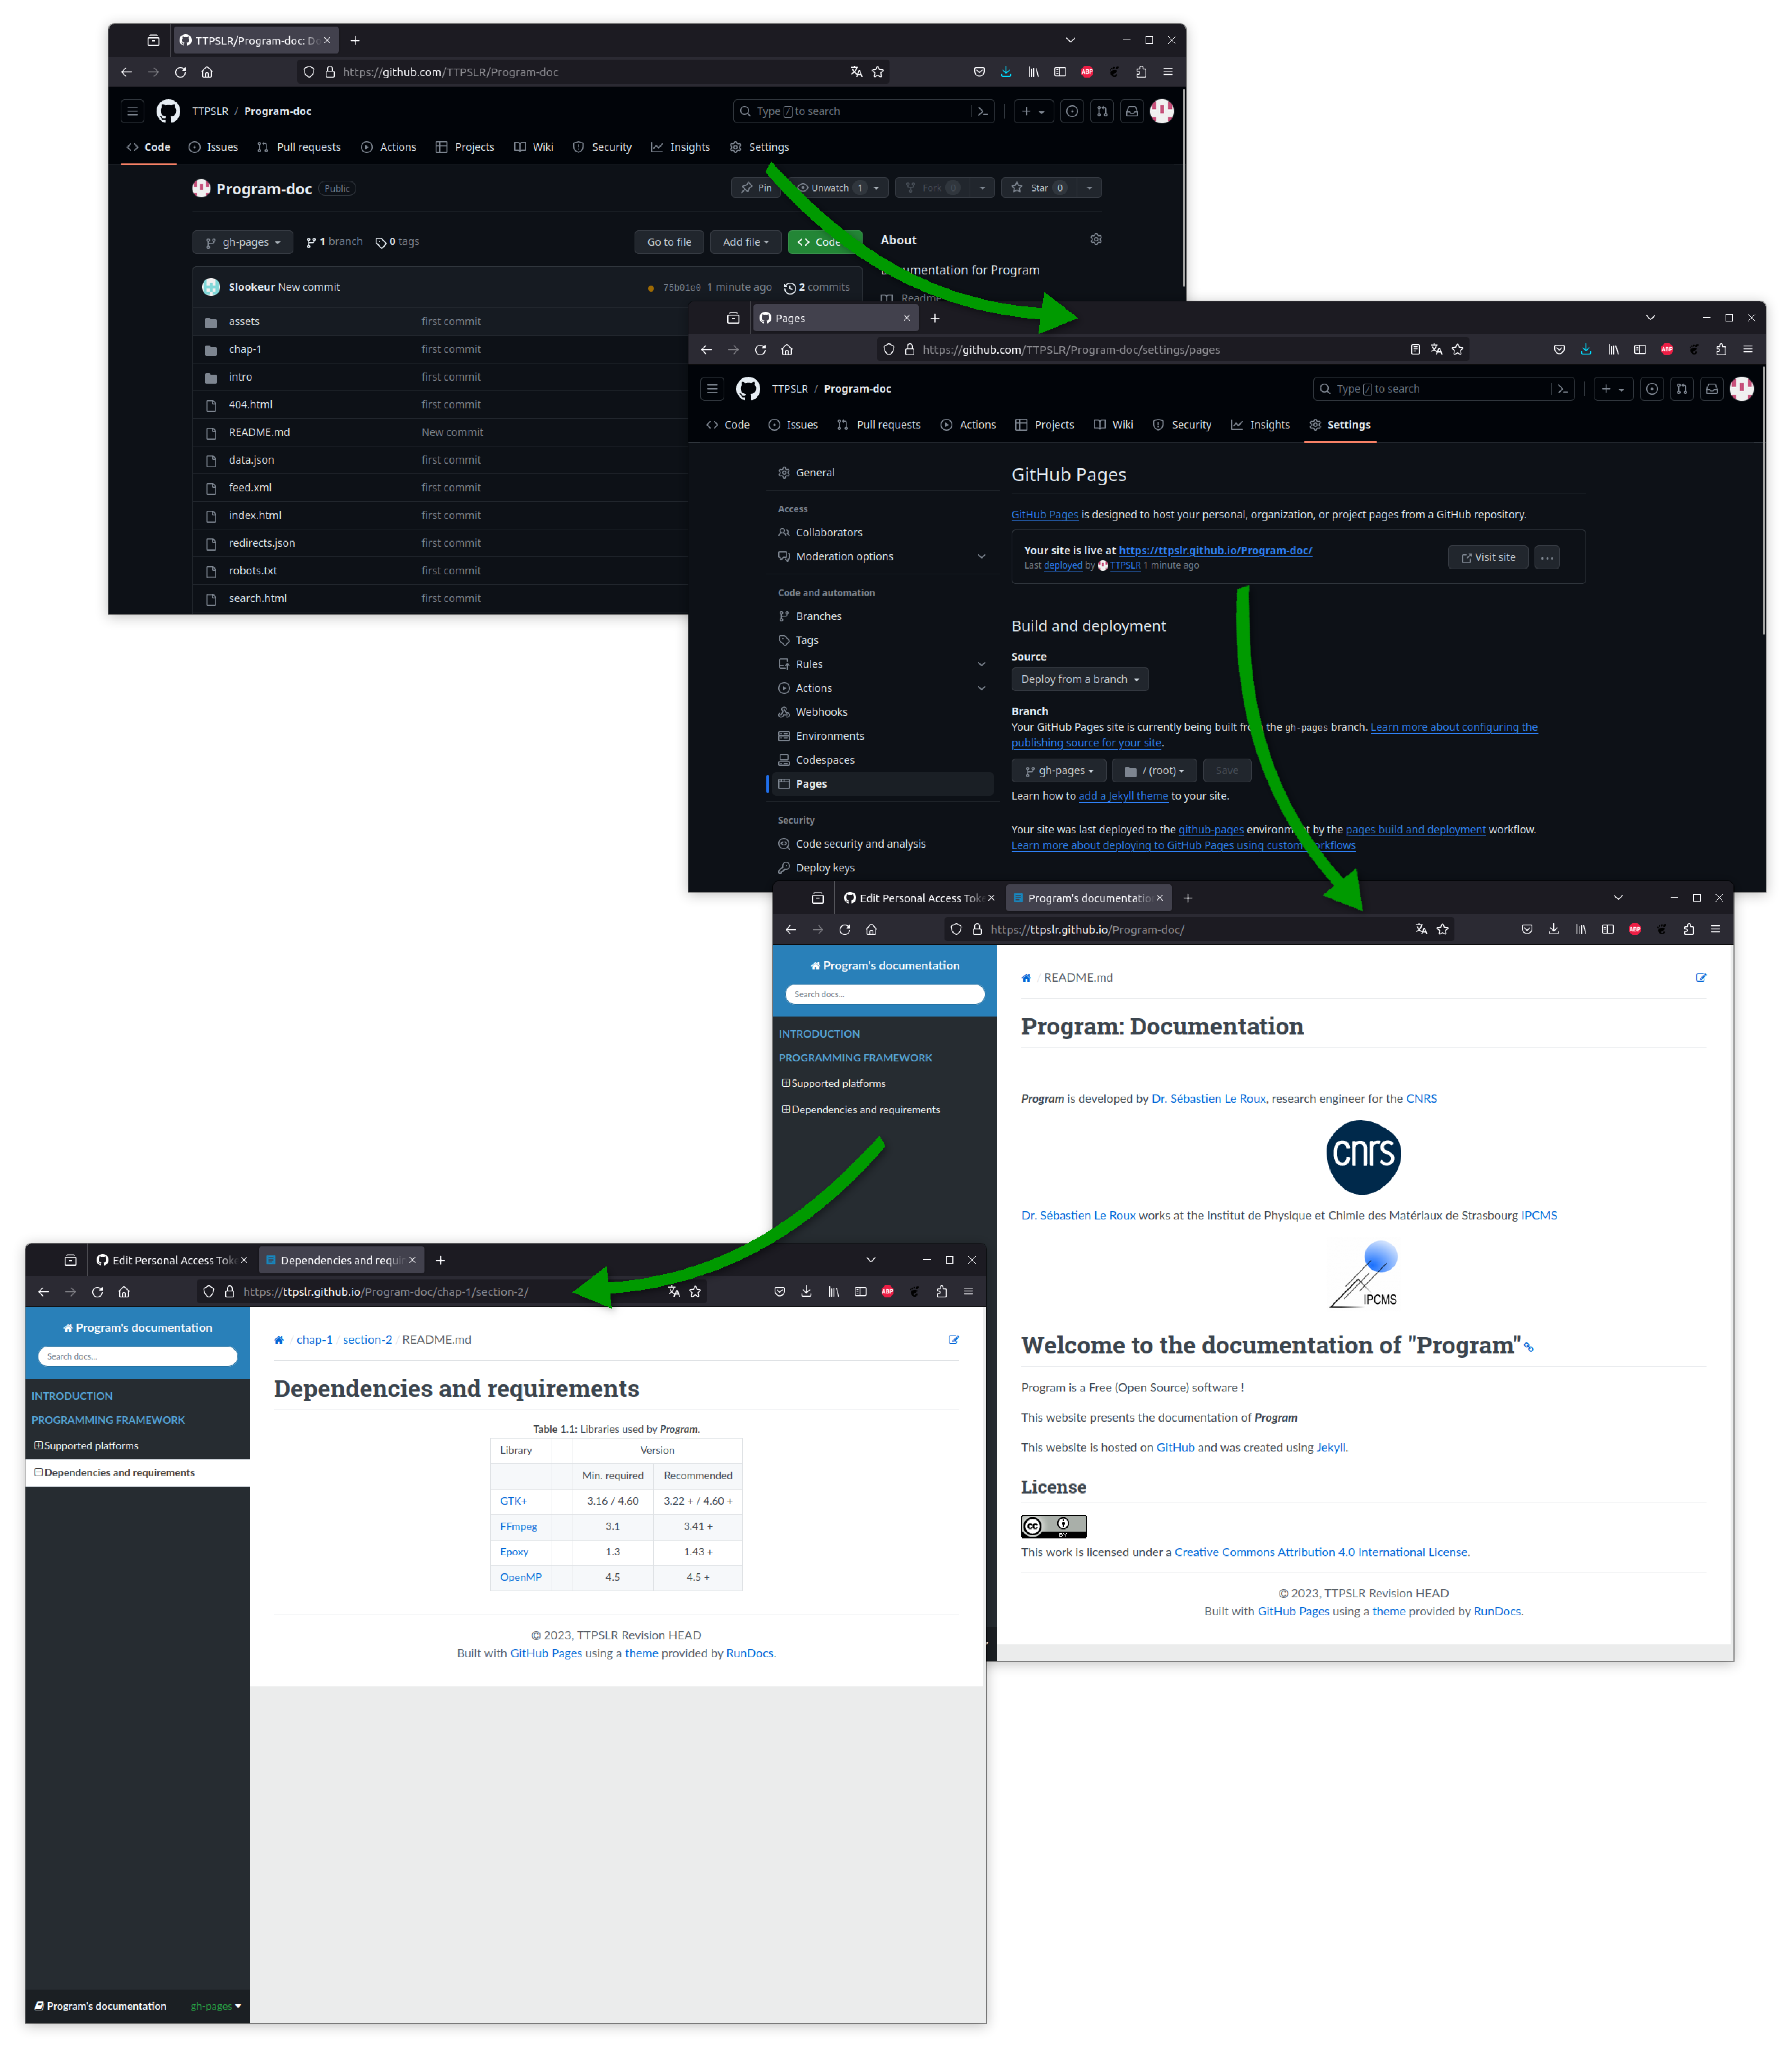
\includegraphics[width=1.0\textwidth,keepaspectratio=true,draft=\ddst]{img/hosts/github/doc.eps} 
\caption{Hosting the documentation on \github\label{dgithub}}
\end{figure}


\include{packaging/packaging}

\chapter*{Conclusion}
\addcontentsline{toc}{chapter}{Conclusion}
\chaptermark{Conclusion}
\markboth{Conclusion}{Conclusion} 

I have been a Linux user for almost 25 year, and a developer for about the same period. \\ 
Back in my beginner's days what really impressed me the most about the Linux ecosystem was the extremely convenient 
way to install softwares: using on-line repositories and automated procedures. \\
It was confidential then, but nowadays thanks to massive usage of smartphones, this has been widely popularised by the words "app store" or "magasin d'applications" (in French). 
For years, and even as impressed as I was by the whole packaging process, I sadly though that all this was out of my league ... until I decided to give it a try.\\[0.25cm]
I hope that this manual helped you understand that this is not out of your league !

\appendix


\chapter{The GNU Autotools files}

\clearpage

\section{The "\bftt{configure.ac}" file}
\label{configall}

{\tiny{
\begin{script}
\confb{AC\_PREREQ}{\red{2.59}}

m4\_define(\bftt{major\_version}, \red{1})
m4\_define(\bftt{minor\_version}, \red{2})
m4\_define(\bftt{patch\_version}, \red{12})
m4\_define(\bftt{version}, \bftt{major\_version}\rtt{.}\bftt{minor\_version}\rtt{.}\bftt{patch\_version})
m4\_define(\bftt{bug\_email}, \red{\email})
m4\_define(\bftt{tar\_name}, \red{program})
m4\_define(\bftt{project\_url}, \red{https://www.program.com})

\confb{AC\_INIT}{\cstr{\bftt{prog}}, \cstr{\bftt{version}}, \cstr{\bftt{bug\_email}}, \cstr{\bftt{tar\_name}}, \cstr{\bftt{project\_url}}}
\confa{AM\_INIT\_AUTOMAKE}

\confb{AC\_DEFINE}{MAJOR\_VERSION, \bftt{major\_version}, \cstr{Program major version}}
\confb{AC\_SUBST}{MAJOR\_VERSION, \bftt{major\_version}}
\confb{AC\_DEFINE}{MINOR\_VERSION, \bftt{minor\_version}, \cstr{Program minor version}}
\confb{AC\_SUBST}{MINOR\_VERSION, \bftt{minor\_version}}
\confb{AC\_DEFINE}{PATCH\_VERSION, \bftt{patch\_version}, \cstr{Program patch version}}
\confb{AC\_SUBST}{PATCH\_VERSION, \bftt{patch\_version}}

\confb{AC\_CHECK\_PROG}{[PKG\_CONFIG], [pkg-config], [yes], [no])}
\confb{AC\_CHECK\_PROG}{[UP\_MIME], [update-mime-database], [yes], [no]}
\confb{AC\_CHECK\_PROG}{[UP\_DESKTOP], [update-desktop-database], [yes], [no]}
\confb{AC\_CHECK\_PROG}{[UP\_APPSTREAM], [appstream-util], [yes], [no]}   

\confb{AC\_DEFUN}{[AX\_CHECK\_COMPILER\_FLAGS],
\tabul [AC\_PREREQ(\red{2.59}) \dnl{for \_AC\_LANG\_PREFIX}
\tabul AC\_MSG\_CHECKING([whether \_AC\_LANG compiler accepts \$1])
\tabul \confb{AS\_LITERAL\_IF}{[\$1],
\tabul\tabul [AC\_CACHE\_VAL(AS\_TR\_SH(ax\_cv\_[]\_AC\_LANG\_ABBREV[]\_flags\_\$1), [
\tabul\tabul\tabul ax\_save\_FLAGS=\$[]\_AC\_LANG\_PREFIX[]FLAGS
\tabul\tabul\tabul \_AC\_LANG\_PREFIX[]FLAGS="\$1"
\tabul\tabul\tabul C\_COMPILE\_IFELSE([AC\_LANG\_PROGRAM()],
\tabul\tabul\tabul AS\_TR\_SH(ax\_cv\_[]\_AC\_LANG\_ABBREV[]\_flags\_\$1)=yes,
\tabul\tabul\tabul AS\_TR\_SH(ax\_cv\_[]\_AC\_LANG\_ABBREV[]\_flags\_\$1)=no)
\tabul\tabul \_AC\_LANG\_PREFIX[]FLAGS=\$ax\_save\_FLAGS])],
\tabul\tabul [ax\_save\_FLAGS=\${[]\_AC\_LANG\_PREFIX[]FLAGS}
\tabul\tabul \_AC\_LANG\_PREFIX[]FLAGS="\$1"
\tabul\tabul AC\_COMPILE\_IFELSE([AC\_LANG\_PROGRAM()],
\tabul\tabul\tabul eval AS\_TR\_SH(ax\_cv\_[]\_AC\_LANG\_ABBREV[]\_flags\_\$1)=yes,
\tabul\tabul\tabul eval AS\_TR\_SH(ax\_cv\_[]\_AC\_LANG\_ABBREV[]\_flags\_\$1)=no)
\tabul\tabul \_AC\_LANG\_PREFIX[]FLAGS=\$ax\_save\_FLAGS]}
\tabul eval ax\_check\_compiler\_flags=\${AS\_TR\_SH}(ax\_cv\_[]\_AC\_LANG\_ABBREV[]\_flags\_\$1)
\tabul AC\_MSG\_RESULT(\$ax\_check\_compiler\_flags)
\tabul if test "x\$ax\_check\_compiler\_flags" = xyes; then
\tabul\tabul m4\_default([\$2], :)
\tabul else
\tabul\tabul m4\_default([\$3], :)
\tabul fi
]}

\confa{AC\_PROG\_CC}
\confb{AX\_CHECK\_COMPILER\_FLAGS}{\cstr{\red{\${CFLAGS}}}}

\confa{AC\_FC\_WRAPPERS}
\confb{AC\_LANG\_PUSH}{\cstr{Fortran}}
\confb{AC\_PROG\_FC}{\cstr{xlf95 fort ifort ifc f95 g95 pgf95 lf95 xlf90 f90 pgf90 gfortran}, 
             \cstr{90}}
\confb{AC\_FC\_SRCEXT}{f90, FCFLAGS\_f90="\${FCFLAGS\_f90} \${FCFLAGS}",
                AC\_MSG\_ERROR(\cstr{Err. comp. .f90})}
\confb{AC\_FC\_SRCEXT}{F90, FCFLAGS\_F90="\${FCFLAGS\_F90} \${FCFLAGS}", 
                AC\_MSG\_ERROR(\cstr{Err. comp. .F90})}
\confb{AX\_CHECK\_COMPILER\_FLAGS}{\cstr{\red{\${FCFLAGS}}}}
\confa{AC\_FC\_LIBRARY\_LDFLAGS}
\confa{AC\_FC\_FREEFORM}
\confb{AC\_LANG\_POP}{\cstr{Fortran}}

\confb{PKG\_CHECK\_MODULES}{\rtt{GTK}, \cstr{\bftt{gtk+-3.0} >= 3.16}}
\confb{PKG\_CHECK\_MODULES}{\rtt{LIBXML2}, \cstr{\bftt{libxml-2.0} >= 2.4.0}}
\confb{PKG\_CHECK\_MODULES}{\rtt{FFMPEG}, \cstr{\bftt{libavcodec libavformat libavutil libswscale}}}
\confb{PKG\_CHECK\_MODULES}{\rtt{GLU}, \cstr{\bftt{glu}}}
\confb{PKG\_CHECK\_MODULES}{\rtt{EPOXY}, \cstr{\bftt{epoxy}}}

\confb{AC\_CONFIG\_FILES}{\cstr{
  \red{Makefile
  src/Makefile}
}}

\confa{AC\_OUTPUT}
\end{script}
}}

\section{The "\bftt{Makefile.am}"}
\label{makeall}
\vspace{-0.75cm}
{\tiny{
\begin{script}
\dgtt{prog\_datadir} = \var{\$(DESTDIR)\$(datadir)}
\dgtt{prog\_docdir} = \var{\$(DESTDIR)\$(docdir)}
\dgtt{prog\_mandir} = \var{\$(DESTDIR)\$(mandir)}
\dgtt{prog\_pkgdatadir} = \var{\$(DESTDIR)\$(pkgdatadir)}
\dgtt{prog\_desktopdir} = \var{\$(prog\_pkgdatadir)}/applications
\dgtt{prog\_metadir} = \var{\$(prog\_pkgdatadir)}/metainfo
\dgtt{SUBDIRS} = src
\dgtt{prog\_docdir} = \var{\$(docdir)}
\dgtt{prog\_doc\_DATA} = README.md AUTHORS ChangeLog
\dgtt{prog\_mandir} = \var{\$(mandir)}/man1/
\dgtt{prog\_man\_DATA} = program.1.gz
\rtt{install-data-local:}
\tabul if test -d \var{\$(srcdir)}/data; then \textbackslash
\tabul \tabul \var{\$(mkinstalldirs) \$(prog\_pkgdatadir)}/data; \textbackslash
\tabul \tabul for data in \var{\$(srcdir)}/data/*; do \textbackslash
\tabul \tabul \tabul if test -f \var{\$\$data}; then \textbackslash
\tabul \tabul \tabul \tabul \var{\$(INSTALL\_DATA) \${data} \$(prog\_pkgdatadir)}/data; \textbackslash
\tabul \tabul \tabul fi \textbackslash
\tabul \tabul done \textbackslash
\tabul fi
\tabul if test -d \var{\$(srcdir)}/pickups; then \textbackslash
\tabul \tabul \var{\$(mkinstalldirs) \$(prog\_pkgdatadir)}/pixmaps; \textbackslash
\tabul \tabul for pixmap in \var{\$(srcdir)}/pixmaps/*; do \textbackslash
\tabul \tabul \tabul if test -f \var{\$\${pixmap}}; then \textbackslash
\tabul \tabul \tabul \tabul \var{\$(INSTALL\_DATA) \$\${pixmap} \$(prog\_pkgdatadir)}/pixmaps; \textbackslash
\tabul \tabul \tabul else \textbackslash
\tabul \tabul \tabul \tabul \var{\$(mkinstalldirs) \$(prog\_pkgdatadir)/\$\${pixmap}}	; \textbackslash
\tabul \tabul \tabul \tabul for pixma in \var{\$\${pixmap}}/*; do \textbackslash
\tabul \tabul \tabul \tabul \tabul if test -f \var{\$\${pixma}}; then \textbackslash
\tabul \tabul \tabul \tabul \tabul \tabul \var{\$(INSTALL\_DATA) \$\${pixma} \$(prog\_pkgdatadir)/\$\${pixmap}}; \textbackslash
\tabul \tabul \tabul \tabul \tabul fi \textbackslash
\tabul \tabul \tabul \tabul done \textbackslash
\tabul \tabul \tabul fi \textbackslash
\tabul \tabul done \textbackslash
\tabul fi
\tabul if [ ! -d \var{\$(prog\_iconsdir)} ]; then \textbackslash
\tabul \tabul \var{\$(mkinstalldirs)} \var{\$(prog\_iconsdir)}; \textbackslash
\tabul fi
\tabul \var{\$(INSTALL\_DATA) \$(srcdir)}/metadata/icons/program.svg \var{\$(prog\_iconsdir)}
\tabul \var{\$(INSTALL\_DATA) \$(srcdir)}/metadata/icons/program-project.svg \var{\$(prog\_iconsdir)}
\tabul \var{\$(INSTALL\_DATA) \$(srcdir)}/metadata/icons/program-workspace.svg \var{\$(prog\_iconsdir)}
\tabul if [ ! -d \var{\$(prog\_mimedir)} ]; then \textbackslash
\tabul \tabul \var{\$(mkinstalldirs)} \var{\$(prog\_mimedir)}; \textbackslash
\tabul fi
\tabul \var{\$(INSTALL\_DATA) \$(srcdir)}/metadata/mime/program.xml \var{\$(prog\_mimedir)}
\tabul if [ ! -d \var{\$(prog\_metadir)} ]; then \textbackslash
\tabul \tabul mkdir -p \var{\$(prog\_metadir)}; \textbackslash
\tabul fi
\tabul \var{\$(INSTALL\_DATA) \$(srcdir)}/metadata/com.program.www.appdata.xml \var{\$(prog\_metadir)}
\tabul if [ ! -d \var{\$(prog\_desktopdir)} ]; then \textbackslash
\tabul \tabul mkdir -p \var{\$(prog\_desktopdir)}; \textbackslash
\tabul fi
\tabul appstream-util validate-relax --nonet \var{\$(prog\_metadir)}/com.program.www.appdata.xml
\tabul desktop-file-install --vendor="" \textbackslash
\tabul \tabul --dir=\var{\$(prog\_desktopdir)} -m 644 \textbackslash
\tabul \tabul \var{\$(prog\_desktopdir)}/program.desktop
\tabul touch --no-create \var{\$(prog\_iconsdir)}
\tabul if [ -u `which gtk-update-icon-cache` ]; then \textbackslash
\tabul \tabul gtk-update-icon-cache -q \var{\$(prog\_iconsdir)}; \textbackslash
\tabul fi
\tabul if [ -z "\var{\$(DESTDIR)}" ]; then \textbackslash
\tabul \tabul update-desktop-database \var{\$(prog\_desktopdir)} &> /dev/null || :; \textbackslash
\tabul \tabul update-mime-database \var{\$(prog\_datadir)}/mime &> /dev/null || :; \textbackslash
\tabul fi
\rtt{uninstall-local:}
\tabul -rm -rf \var{\$(prog\_pkgdatadir)}/data/*
\tabul -rmdir \var{\$(prog\_pkgdatadir)}/data
\tabul -rm -rf \var{\$(prog\_pkgdatadir)}/pixmaps/*
\tabul -rmdir \var{\$(prog\_pkgdatadir)}/pixmaps
\tabul -rm -rf \var{\$(prog\_pkgdatadir)}/pixmaps/*
\tabul -rmdir \var{\$(prog\_pkgdatadir)}
\tabul -rmdir \var{\$(prog\_docdir)}
\tabul -rm -rf \var{\$(prog\_iconsdir)}/program.svg
\tabul -rm -rf \var{\$(prog\_iconsdir)}/program-project.svg
\tabul -rm -rf \var{\$(prog\_iconsdir)}/program-workspace.svg
\tabul -rm -f \var{\$(prog\_desktopdir)}/program.desktop
\tabul -rm -f \var{\$(prog\_metadir)}/com.program.www.appdata.xml
\tabul touch --no-create \var{\$(prog\_iconsdir)}
\tabul if [ -u `which gtk-update-icon-cache` ]; then \textbackslash
\tabul \tabul gtk-update-icon-cache -q \var{\$(prog\_iconsdir)}; \textbackslash
\tabul fi
\tabul if [ -z "\var{\$(DESTDIR)}" ]; then \textbackslash
\tabul \tabul update-desktop-database \var{\$(prog\_desktopdir)} &> /dev/null || :; \textbackslash
\tabul \tabul update-mime-database \var{\$(prog\_datadir)}/mime &> /dev/null || :; \textbackslash
\tabul fi
\end{script}
}}

\section{The "\bftt{src/Makefile.am}"}
\label{makeall}

{\scriptsize{
\begin{script}
\bad{bin\_PROGRAMS} = prog

\dgtt{prog\_LDADD} = \var{\$(GTK\_LIBS) \$(LIBXML2\_LIBS) \$(PANGOFT2\_LIBS) \$(FFMPEG\_LIBS) \$(GLU\_LIBS) \$(EPOXY\_LIBS)}

\dgtt{LIB\_CFLAGS} = \var{\$(GTK\_CFLAGS) \$(LIBXML2\_CFLAGS) \$(PANGOFT2\_CFLAGS) \$(FFMPEG\_CFLAGS) \$(GLU\_CFLAGS) \$(EPOXY\_CFLAGS)}

\dgtt{OpenMP\_FLAGS} = -DOPENMP -fopenmp
\dgtt{AM\_LDFLAGS} = \var{\$(OpenMP\_FLAGS)}
\dgtt{AM\_CPPFLAGS} = \var{\$(OpenMP\_FLAGS)}
\dgtt{AM\_FFLAGS} = \var{\$(OpenMP\_FLAGS)}
\dgtt{AM\_CFLAGS} = -DGDK\_DISABLE\_DEPRECATED \var{\$(OpenMP\_CFLAGS) \$(LIB\_CFLAGS)}

\dgtt{prog\_fortran\_files} = file-1.f90 file-2.f90
\dgtt{prog\_fortran\_modules} = mod.f90

\dgtt{prog\_fortran} = \var{\$(prog\_fortran\_modules) \$(prog\_fortran\_files)}
\var{\$(patsubst \%.F90,\%.o,\$(prog\_fortran\_files)): \$(patsubst \%.F90,\%.o,\$(prog\_fortran\_modules))}

\dgtt{prog\_c} = main.c gui.c

\rtt{clean:}
\tabul -rm -f *.mod
\tabul -rm -f */*.o

\dgtt{prog\_SOURCES} = \var{\$(prog\_fortran)} \var{\$(prog\_c)}
\end{script}
}}

\chapter{The packaging files}

\clearpage

\section{"\bftt{.spec}" file for RPM packaging}
\label{spec}
\vspace{-1cm}
{\scriptsize{
\begin{script}
\bad{Name:}      prog
\bftt{\%global} \var{upname} Program
\bad{Version:}   1.2.12
\bad{Release:}   3\var{\%\{?dist\}}
\bad{Summary:}   An nice program
\bad{License:}   AGPL-3.0-or-later
\bad{Source0:}   \gitauth/\%\{upname\}/archive/refs/tags/v\var{\%\{version\}}.tar.gz
\comm{Source1:   ./v\%\%\{version\}.tar.gz.asc}
\comm{Source2:   \%\%\{name\}.gpg}
\bad{URL:}        https://www.\var{\%\{name\}}.com/

\bad{BuildRequires:} make
\bad{BuildRequires:} automake
\bad{BuildRequires:} autoconf
\bad{BuildRequires:} pkgconf-pkg-config
\bad{BuildRequires:} gcc
\bad{BuildRequires:} gcc-gfortran
\bad{BuildRequires:} libgfortran
\bad{BuildRequires:} pkgconfig(gtk+-3.0)
\bad{BuildRequires:} pkgconfig(libxml-2.0)
\bad{BuildRequires:} pkgconfig(glu)
\bad{BuildRequires:} pkgconfig(epoxy)
\bad{BuildRequires:} pkgconfig(libavutil)
\bad{BuildRequires:} pkgconfig(libavcodec)
\bad{BuildRequires:} pkgconfig(libavformat)
\bad{BuildRequires:} pkgconfig(libswscale)
\bad{BuildRequires:} desktop-file-utils
\bad{BuildRequires:} libappstream-glib
\comm{BuildRequires: gnupg2}
\bad{Requires:} gtk3
\bad{Requires:} mesa-libGLU

\dgtt{\%prep}
\comm{\%\%\{gpgverify\} --keyring='\%\%\{SOURCE2\}' --signature='\%\%\{SOURCE1\}' --data='\%\%\{SOURCE0\}'}
\bftt{\%autosetup} -n \var{\%\{upname\}}-\var{\%\{version\}}

\dgtt{\%build}
\bftt{\%configure}
\bftt{\%make\_build}

\dgtt{\%install}
\bftt{\%make\_install}

\dgtt{\%check}
desktop-file-validate \var{\%\{buildroot\}}/\var{\%\{\_datadir\}}/applications/\var{\%\{name\}}.desktop
appstream-util validate-relax --nonet \var{\%\{buildroot\}}\var{\%\{\_metainfodir\}}/com.\var{\%\{name\}}.www.appdata.xml

\dgtt{\%files}
\bftt{\%license} COPYING
\var{\%\{\_bindir\}}/\var{\%\{name\}}
\var{\%\{\_datadir\}}/\var{\%\{name\}}
\var{\%\{\_datadir\}}/doc/\var{\%\{name\}}
\var{\%\{\_mandir\}}/man1/\var{\%\{name\}}.1*
\var{\%\{\_datadir\}}/applications/\var{\%\{name\}}.desktop
\var{\%\{\_metainfodir\}}/com.\var{\%\{name\}}.www.appdata.xml
\var{\%\{\_datadir\}}/mime/packages/\var{\%\{name\}}.xml
\var{\%\{\_datadir\}}/pixmaps/\var{\%\{name\}}.svg
\var{\%\{\_datadir\}}/pixmaps/\var{\%\{name\}}-program.svg
\var{\%\{\_datadir\}}/pixmaps/\var{\%\{name\}}-workspace.svg

\dgtt{\%changelog}
* Thu Mar 30 2023 Your Name <\email> - \gtt{1.2.12}-\rtt{3}
- Revised package: what you did here.
\end{script}
}}

\section{"\texttt{debian}" directory for Debian packaging}

%\subsection{The "\texttt{changelog}" file}

%\subsection{The "\texttt{control}" file}

\subsection{The "\texttt{copyright}" file}
\label{acopy}
{\notsotiny{
\input{copyright}
}}

\subsection{Example script to build and test locally your Debian package}
\label{btdebs}

{\tiny{
\begin{script}
\bash

\func{autoclean}
  \brm \violet{-f} aclocal.m4
  \brm \violet{-rf} auto4te.cache
  \brm \violet{-f} configure~
  aclocal
  autoconf
  automake \violet{--add-missing}
  \brm \violet{-f} configure~
\efunc

\var{VERSION}=\say{1.2.12}

\comm{Ensure that the top directory is clean}
\brm \violet{-f} \bap*\_\bap\dvar{VERSION}\bap*\bap
\bif \violet{-d} program-\dvar{VERSION} \then
  \brm \violet{-rf} program-\dvar{VERSION}
\bfi

\var{DOWN}\bad{=}\magenta{1}
\bif \dvar{DOWN} \beq \magenta{1} \then
  \comm{Retrieving the sources of the program from the official repository}
  \bad{wget} \gitprog/archive/refs/tags/v\dvar{VERSION}.tar.gz
  \bad{tar} \violet{-zxf} v\dvar{VERSION}.tar.gz
  \mv Program-\dvar{VERSION} program-\dvar{VERSION}
  \brm v\dvar{VERSION}.tar.gz
\bfi

\var{BUILD}\bad{=}\magenta{1}
\bif \dvar{BUILD} \beq \magenta{1} \then
  \cd program-\dvar{VERSION}
  \comm{If the 'debian' directory is not shipped with the official tarball}
  \comm{Uncomment and adapt the next line to add the 'debian' directory in the sources directory}
  \comm{cp -r ../debian-package-data debian}

  \comm{Ensure that there is a README file}
  \bcp README.md README

  \comm{To ensure that the version of the autotools files are suitable for this system}
  autoclean
  \comm{Debian packager identification}
  \bad{export} \dctt{DEBEMAIL}\bad{=}\say{\email}
  \bad{export} \dctt{DEBFULLNAME}\bad{=}\say{Your Name}
  \comm{Improved lintian command for package verification}
  \bad{alias} \dctt{lintian}\bad{=}\reg{lintian -EviIL +pedantic --color auto}
  \comm{Creating the Debian origin tarball}
  \bftt{dh\_make} \violet{--createorig -s -y}
  \comm{Building the Debian package}
  \bftt{dpkg-buildpackage}
  \cd ..
\bfi

\var{TEST}\bad{=}\magenta{1}
\bif \dvar{TEST} \beq \magenta{1} \then
  \comm{Linitian on 'program.changes'}
  \lint ./program\_*changes \bad{>&} results.lintian
  \cd program-\dvar{VERSION}
  \comm{Licensecheck to check for license}
  \bftt{licensecheck} \violet{--recursive --copyright} \btt{.} \bad{>&} ../license.check
  \comm{Scan-copyrights to create a copyrights file from scratch using licensecheck}
  \bftt{scan-copyrights} \bad{>&} ../scan.copy
  \cd ..
\bfi
 
\var{PIUPARTS}\bad{=}\magenta{0}
\bif \dvar{PIUPARTS} \beq \magenta{1} \then
  \echo \say{Piuparts on program.deb} \bad{>} results.piuparts
  \echo \say{ } \bad{>>} results.piuparts
  \piup ./program\_\dvar{VERSION}*.deb \bad{&>>} results.piuparts
  \echo \say{ } \bad{>>} results.piuparts
  \echo \say{Piuparts on program-data.deb} \bad{>>} results.piuparts
  \echo \say{ } \bad{>>} results.piuparts
  \piup ./program-data*.deb \bad{&>>} results.piuparts
\bfi
\end{script}

}}

\subsection{Example of ITP bug report message}
\label{bugreport}

{\footnotesize{
\begin{script}
\magenta{Subject: ITP: }\bftt{program} \magenta{--} \bftt{short description}
\bad{Package: wnpp}
\bad{X-Debbugs-Cc:} \magenta{debian-devel@lists.debian.org}
\bad{Owner: }\bftt{Your Name \magenta{<\email>}}
\bad{Severity: wishlist}

* Package name    : \bftt{program}
  Version         : \bftt{1.2.12}
  Upstream Author : \bftt{Your Name \magenta{<\email>}}
* URL             : \red{https://www.program.com/}
* License         : AfferoGPLv3+
  Programming Lang: C, Fortran90, GLSL
  Description     : \bftt{short description}

"program" is a cross-platform software doing many things, 
and I will elaborate about the most significant achievements now ...

Among the many reasons I could think of, to help you understand why you
should consider "program" seriously, I will pick 3: 

1) This is the first reason ...

2) This is the second reason ...

3) This is the third reason ...

For the time being "program" is being maintained by ..

Sources are hosted on Github and Salsa:

"program" sources:          \gitprog
"program" sources on Salsa: https://salsa.debian.org/author/program

Finally I am looking for a sponsor. 
Indeed as this is my first Debian package, I am looking for all the help I can get. 
I am willing to spend time to learn how to do things properly 
to get "program" approved by the Debian community and ultimately packaged. 
If the proper way to do that is inside a packaging team then after checking 
the packaging teams at \href{https://wiki.debian.org/Teams}{https://wiki.debian.org/Teams} 
I think the "Debian *** Team" is likely to be the most appropriate place to start.

Best regards.

Your Name
\end{script}
}}

\section{Metadata for Linux intergation}

\subsection{Custom MIME file(s) setup}
\label{mime}

This file is required to define file association(s) and uses the \texttt{XML} file format:
{\scriptsize{
\begin{script}
\dbtt{<?xml}? \abtt{version=}\red{"1.0"} \abtt{encoding=}\red{"UTF-8"}\dbtt{?>}
\dbtt{<mime-info} \abtt{xmlns=}\red{"http://www.freedesktop.org/standards/shared-mime-info"}\dbtt{>}
  \dbtt{<mime-type} \abtt{type=}\red{"application/x-ppf"}\dbtt{>}
    \dbtt{<comment>}Program Project file\dbtt{</comment>}
    \dbtt{<glob} \abtt{pattern=}\red{"*.ppf"}\dbtt{/>}
    \dbtt{<generic-icon} \abtt{name=}\red{"program-project"}\dbtt{/>}
    \dbtt{<sub-class-of} \abtt{type=}\red{"text/plain"}\dbtt{/>}
  \dbtt{</mime-type>}
  \dbtt{<mime-type} \abtt{type=}\red{"application/x-pwf"}\dbtt{>}
    \dbtt{<comment>}Program Workspace file\dbtt{</comment>}
    \dbtt{<glob} \abtt{pattern=}\red{"*.pwf"}\dbtt{/>}
    \dbtt{<generic-icon} \abtt{name=}\red{"program-workspace"}\dbtt{/>}
    \dbtt{<sub-class-of} \abtt{type=}\red{"application/octet-stream"}\dbtt{/>}
  \dbtt{</mime-type>}
\dbtt{</mime-info>}
\end{script}
}}
\\
\noindent Each file association is defined between the \dbtt{<mime-type>}  ... \dbtt{</mime-type>} tags:
{\scriptsize{
\begin{script}
...
  \dbtt{<mime-type} \abtt{type=}\red{"application/x-ppf"}\dbtt{>}
    \dbtt{<comment>}Program Project file\dbtt{</comment>}
    \dbtt{<glob} \abtt{pattern=}\red{"*.ppf"}\dbtt{/>}
    \dbtt{<generic-icon} \abtt{name=}\red{"program-project"}\dbtt{/>}
    \dbtt{<sub-class-of} \abtt{type=}\red{"text/plain"}\dbtt{/>}
  \dbtt{</mime-type>}
... 
\end{script}
}}
\noindent Where the tags are used as follow:
\begin{itemize}
\item \dbtt{<comment>}: to describe the file format.
\item \dbtt{<glob}: to define the file extension.
\item \dbtt{<generic-icon}: to define the icon name, without extension (svg, png). \\
In the example providing that the file "\texttt{program-project.svg}" exists and is located in "\texttt{/usr/share/pixmaps}", 
then it is enough for the system to find it and associate it with the file format.
\item \dbtt{<sub-class-of}: to help the system recognize the format:
\begin{itemize}
\item \red{\texttt{"text/plain"}} for text formats.
\item \red{\texttt{"application/octet-stream"}} for binary formats.
\end{itemize}
\end{itemize}
\noindent To get information about the format of \texttt{this\_file}: 
\vspace{-0.25cm}
\begin{script}
\fprompt{~} \bftt{gio} \rtt{info} this\_file
\end{script}

\subsection{Desktop entry for desktop application}
\label{desktop}

The following is an example of the content of a installed "\bftt{*.desktop}" file. 
{\scriptsize{
\begin{script}
\dgtt{[Desktop Entry]}
\dctt{Version}=\violet{1.0}
\dctt{Name}=Program
\dctt{GenericName}=Program
\dctt{Comment}=For more information: https://www.program.com/
\dctt{Comment}\aqua{[fr]}=Pour plus d'information: https://www.program.com/
\dctt{Comment}\aqua{[es]}=Para más información: https://www.program.com/
\dctt{Keywords}=chemistry;physics;
\dctt{Keywords}\aqua{[fr]}=chimie;physique;
\dctt{Keywords}\aqua{[es]}=química;física;
\dctt{Exec}=program \violet{\%F}
\comm{Providing that the file "program.svg" exists and is located in "/usr/share/pixmaps"}
\comm{Then it is enough for the system to find it and associate it using:}
\dctt{Icon}=propram
\dctt{Terminal}=\violet{false}
\dctt{Type}=Application
\dctt{MimeType}=application/x-ppf;application/x-pwf;
\dctt{StartupNotify}=\violet{true}
\dctt{Categories}=Education;Science;Chemistry;Physics;
\end{script}
}}
\\
\noindent For \dctt{MimeType} the keywords must match the values defined in the MIME association file by the \dbtt{<mime-type }\abtt{type=}\red{"keyword"}\dbtt{>}
 opening tags, see [Sec.~\ref{mime}].

\clearpage
\subsection{AppStream metadata for desktop application}
\label{appstream}
\vspace{-0.5cm}
{\notsotiny{
\begin{script}
\dbtt{<?xml}? \abtt{version=}\red{"1.0"} \abtt{encoding=}\red{"UTF-8"}\dbtt{?>}
<!-- This is a commented line for a XML file -->
<!-- Copyright 2023 Your Name -->
<!-- The type of desktop object described -->
\dbtt{<component} \abtt{type=}\red{"desktop-application"}\dbtt{>}

  \dbtt{<id>}com.program.www\dbtt{</id>}
  \dbtt{<name>}Program\dbtt{</name>}
  \dbtt{<summary>}An interesting program\dbtt{</summary>}
  <!-- The license of your program --> 
  \dbtt{<project\_license>}AGPL-3.0-or-later\dbtt{</project\_license>}
  \dbtt{<metadata\_license>}FSFAP\dbtt{</metadata\_license>}
  
  \dbtt{<description>}
    \dbtt{<p>}Program: an utility to do many things !\dbtt{</p>}
  \dbtt{</description>}
  <!-- The desktop file that describes launch information --> 
  \dbtt{<launchable} \abtt{type=}\red{"desktop-id"}\dbtt{>}program.desktop\dbtt{</launchable>}

  <!-- Up to 3 screenshot(s), used in the Linux app store to illustrate your program -->
  \dbtt{<screenshots}
    \dbtt{<screenshot>}
      <!-- The video cannot be the default screenshot -->
      <!-- Container: mkv, Video codecs allowed: av1 or vp9, Audio codec allowed: opus -->
      \dbtt{<caption>}A nice video to illustrate the features of the program\dbtt{</caption>}
      \dbtt{<video} \abtt{container=}\red{"webm"} \abtt{codec=}\red{"vp9"} \abtt{width=}\red{"1920"} \abtt{height=}\red{"1080"}\dbtt{>}https://www.program.com/my-video.webm\dbtt{</video>}
    \dbtt{</screenshot}
    \dbtt{<screenshot} \abtt{type=}\red{"default"}\dbtt{>}
      \dbtt{<caption>}Overview of the program\dbtt{</caption>}
      \dbtt{<image} \abtt{type=}\red{"source"} \abtt{width=}\red{"1600"} \abtt{height=}\red{"900"}\dbtt{>}https://www.program.com/program-overview.png\dbtt{</image>}
    \dbtt{</screenshot}
    \dbtt{<screenshot>}
      \dbtt{<caption>}A detail of the program\dbtt{</caption>}
      \dbtt{<image} \abtt{type=}\red{"source"} \abtt{width=}\red{"1600"} \abtt{height=}\red{"900"}\dbtt{>}https://www.program.com/program-detail.png\dbtt{</image>}
    \dbtt{</screenshot}
    \dbtt{<screenshot>}
      \dbtt{<caption>}Another detail of the program\dbtt{</caption>}
      \dbtt{<image} \abtt{type=}\red{"source"} \abtt{width=}\red{"1600"} \abtt{height=}\red{"900"}\dbtt{>}https://www.program.com/program-other-detail.png\dbtt{</image>}
    \dbtt{</screenshot}
  \dbtt{</screenshots}
  
  \dbtt{<url} \abtt{type=}\red{"homepage"}\dbtt{>}https://www.program.com/\dbtt{</url>}
  \dbtt{<url} \abtt{type=}\red{"bugtracker"}\dbtt{>}\gitprog/issues/new/choose\dbtt{</url>}
  \dbtt{<developer\_name>}Mr. Your Name\dbtt{</developer\_name>}
  \dbtt{<update\_contact>}\metamail\dbtt{</update\_contact>}
  
  \dbtt{<provides>}
    \dbtt{<binary>}program\dbtt{</binary>}
  \dbtt{</provides>}
 
  \dbtt{<keywords>}
    \dbtt{<keyword>}chemistry\dbtt{</keyword>}
    \dbtt{<keyword>}physics\dbtt{</keyword>}
    \dbtt{<keyword} \abtt{xml:lang=}\red{"fr"}\dbtt{>}chimie\dbtt{</keyword>}
    \dbtt{<keyword} \abtt{xml:lang=}\red{"fr"}\dbtt{>}physique\dbtt{</keyword>}
    \dbtt{<keyword} \abtt{xml:lang=}\red{"es"}\dbtt{>}química\dbtt{</keyword>}
    \dbtt{<keyword} \abtt{xml:lang=}\red{"es"}\dbtt{>}física\dbtt{</keyword>}
  \dbtt{</keywords>}

  \dbtt{<content\_rating type}=\red{"oars-1.1}" \dbtt{/>}
  
  \dbtt{<releases>}
    \dbtt{<release} \abtt{version=}\red{"1.2.12"} \abtt{date=}\red{"2023-03-29"}\dbtt{>}
      \dbtt{<description>}
        \dbtt{<p>}Release of version 1.2.12:\dbtt{</p>}
        \dbtt{<p>}- Bug corrections, for details see: \dbtt{<url>}\gitprog/releases/tag/v1.2.12\dbtt{</url>}\dbtt{</p>}
        \dbtt{<p>}- Improvements, for details see: \dbtt{<url>}\gitprog/releases/tag/v1.2.12\dbtt{</url>}\dbtt{</p>}
      \dbtt{</description>}
    \dbtt{</release>}	  
    \dbtt{<release} \abtt{version=}\red{"1.2.11"} \abtt{date=}\red{"2023-02-06"}\dbtt{>}
      \dbtt{<description>}
        \dbtt{<p>}Release of version 1.2.11:\dbtt{</p>}
        \dbtt{<p>}- Bug corrections, for details see: \dbtt{<url>}\gitprog/releases/tag/v1.2.11\dbtt{</url>}\dbtt{</p>}
      \dbtt{</description>}
    \dbtt{</release>}
  \dbtt{</releases>}
  
\dbtt{</component>}
\end{script}
}}


\normalem

%%%%%%%%%%%%%%%%%%%%%%%%%%%%%% Biblio %%%%%%%%%%%%%%%%%%%%%%%%%%%%%%
%\bibliographystyle{these}
%\bibliography{full-biblio}

% Colophon
\colophon{This document has been prepared using the Linux operating system and free softwares:
\begin{tabular}{lc}
The text editor & "\href{https://www.vim.org/}{gVim}" \\
The vector graphics editor & \href{https://inkscape.org/}{Inkscape} \\
The GNU image manipulation program & "\href{https://www.gimp.org/}{GIMP}" \\
And the document preparation system & "\href{https://www.latex-project.org/}{\LaTeXe}".
\end{tabular}}

\end{document}
